\documentclass[a4paper, 12pt, oneside]{report}
\usepackage[T1]{fontenc}
\usepackage[utf8]{inputenc}
\usepackage{lmodern}
\usepackage{layout}
\usepackage{emptypage}
\usepackage{fancyhdr}
\usepackage[spanish,activeacute]{babel}
%\usepackage[Conny]{fncychap}
%\usepackage{graphicx}
\usepackage{subfigure} % subfiguras
\usepackage{caption}
\usepackage{mathtools}
\usepackage{hyperref}
\usepackage[a4paper,top=3cm, bottom=3cm, inner=2.5cm, outer=2.5cm]{geometry}
\usepackage{listings}
\usepackage[spanish]{babel}
\usepackage{url}
\usepackage{float}
\usepackage{multirow}
\usepackage{rotating} 
\usepackage{color}
\usepackage{colortbl}
\usepackage[table]{xcolor}
\usepackage[spanish]{babel}
\usepackage{enumerate}
\usepackage{enumitem}
\usepackage{multicol}
\usepackage{mwe}
\usepackage{listings}
\usepackage[acronym, nonumberlist]{glossaries}
\makeglossaries

%Para que no parta las palabras
\pretolerance=10000
\renewcommand{\lstlistingname}{Cuadro}


\definecolor{backcolour}{rgb}{0.99,0.87,0.46}
 
\lstdefinestyle{mystyle}{
    backgroundcolor=\color{backcolour},
}

\lstset{style=mystyle}


\makeatletter
\renewcommand{\@makeschapterhead}[1]{%
%  \vspace*{50\p@}%
  \vspace*{0\p@}%
  {\parindent \z@ \raggedright
    \normalfont
    \interlinepenalty\@M
    \Huge \bfseries  #1\par \nobreak
%    \vskip 40\p@
    \vskip 15\p@
  }}
\makeatother

\renewcommand{\baselinestretch}{1.4}
\setlength{\headheight}{16pt} 
\captionsetup{justification=justified}
\pretolerance=1000

\chead[]{}
\rhead[]{}
\renewcommand{\headrulewidth}{0.5pt}

\pagestyle{empty}

\title{Herramientas robóticas con tecnologías web en la plataforma Jderobot}
\author{Roberto Pérez González}

\lstset{
	float=hbp,
	basicstyle=\ttfamily\small,
	columns=flexible,
	tabsize=4,
	frame=single,
	extendedchars=true,
	showspaces=false,
	showstringspaces=false,
	numbers=none,
	numberstyle=\tiny,
	breaklines=false,
	breakautoindent=true,
	captionpos=b
}
\setcounter{tocdepth}{4}
\setcounter{secnumdepth}{4}


\begin{document}
%%%%%%%%%%%%%%% Portada %%%%%%%%%%%%%%%%%%%%
\begin{titlepage}
	\begin{center}
		\vspace*{3mm}
		\begin{center}
			
\includegraphics[width=0.8\linewidth]{figures/logo.jpg}
		\end{center}
		\vspace{6.5mm}
		
		\fontsize{15.5}{14}\selectfont ESCUELA TÉCNICA SUPERIOR DE INGENIERÍA DE TELECOMUNICACIÓN
		\vspace{13mm}
		
		\fontsize{14}{14}\selectfont GRADO EN INGENIERÍA EN SISTEMAS \\ AUDIOVISUALES Y MULTIMEDIA
		
		\vspace{55pt}
		
		\fontfamily{lmss}\fontsize{15.7}{14}\selectfont \textbf{TRABAJO FIN DE GRADO} 
		
		\vspace{25mm}
		\begin{huge}
			Por Definir
		\end{huge}
		
		\vspace{25mm}
		
		\begin{large}
			Autor: Roberto Pérez González
			
			Tutor: José María Cañas Plaza
			
			\vspace{10mm}
		\end{large}
		\begin{normalsize}
			Curso académico 2018/2019		
		\end{normalsize}
		\vspace{10mm}
		
	\end{center}
	
\end{titlepage}




\pagenumbering{Roman}

%%%%%%%%%%%%%%% Agradecimientos %%%%%%%%%%%%
\chapter*{Agradecimientos}
\setlength{\parskip}{1ex}



%%%%%%%%%%%%%%% Resumen %%%%%%%%%%%%%%%%%%%%
\chapter*{Resumen}
\setlength{\parskip}{1ex}
La plataforma JdeRobot nació como un paquete de softwares para el desarrollo de aplicaciones robóticas y visión artificial. El propósito de la plataforma es crear herramientas y controladores que faciliten la conexión con componentes hardware. La plataforma esta principalmente desarrollada en C++ y Python.

El propósito de este proyecto es facilitar el uso de las diferentes aplicaciones mediante el uso de tecnologías web en el front-end. Esta tecnología nos permite la ejecución de las diferentes herramientas con independencia del sistema operativo en que se está ejecutando. Además, utilizando el framework Electron, seremos capaces de crear aplicaciones de escritorio evitando de este modo problemas de compatibilidades entre los diferentes navegadores web que hay actualmente.

El desarrollo de este proyecto se realizará utilizando JavaScript, HTML5 y CSV en el cliente, y NodeJS en el servidor, sobre el cual está implementada la tecnología de Electron. Además me apoyare en los middleware ZeroC ICE y ROS para la interconexión cliente-servidor. 

La primera parte del proyecto está centrada en la adaptación de los Visores existentes en la plataforma JdeRobot para que funcionen como aplicaciones de escritorio. Estos visores son Turtlebotviz, Droneviz y  Camviz. Para finalizar esta parte, me centrare en este último visor para hacerlo funcionar con los dos principales middleware de comunicación: ZeroC ICE (como hasta ahora) y ROS.

La segunda parte, consiste en la creación de un nuevo visor web que mostrara objetos 3D, desde un simple punto o segmento, hasta objetos más complejos que se obtienen a partir de modelos 3D. Una de las funciones de este visor es la de ser utilizado en la práctica de JdeRobot Academy “Reconstrucción 3D”.

El último propósito de este proyecto es la elaboración de un nuevo componente para la plataforma JdeRobot. Este nuevo componente será un servidor de imágenes obtenidas a través de cámaras web y servidas a los diferentes visores. Este componente utiliza como middleware de comunicación ROS.

\cleardoublepage

%%%%%%%%%%%%%%% Índices %%%%%%%%%%%%%%%%%%%%
%\cleardoublepage
\renewcommand{\tablename}{Tabla}
%\renewcommand{\listtablename}{Índice de tablas}
%\tableofcontents

%\cleardoublepage % Í­ndice de figuras
%\addcontentsline{toc}{chapter}{\listfigurename}
%\listoffigures

%\cleardoublepage % Í­ndice de tablas
%\addcontentsline{toc}{chapter}{Índice de tablas}
%\listoftables 
\cleardoublepage
\tableofcontents % indice de contenidos

%\cleardoublepage
%\listoffigures % indice de figuras
%\addcontentsline{toc}{chapter}{\'Indice de figuras} % para que aparezca en el indice de contenidos

%%%%%%%%%%%%%%% Acronimos %%%%%%%%%%%%%%%%%%%%
%\addcontentsline{toc}{chapter}{Acr\'onimos}
\chapter*{Acrónimos}

%%%%%%%%%%%%%%% Capí­tulos %%%%%%%%%%%%%%%%%%
\pagestyle{fancy}
\pagenumbering{arabic}
\setlength{\parindent}{6mm}

\lhead[]{CAP\'ITULO \thechapter. INTRODUCCI\'ON}
\chapter{Introducción}\label{cap.introduccion}
En este primer capítulo se tratará de explicar el contexto de las bases tecnológicas en las que se apoya este proyecto, que son principalmente las tecnologías web y la robótica. Para empezar se hablará sobre el estado actual de la robótica y la gran expansión de la misma en nuestros días. Se continuará señalando el contexto de las tecnologías web y como de importantes son en la sociedad actual, para continuar explicando su arquitectura y las tecnologías más importantes. Para finalizar este capitulo, se introducirá en Jderobot y en los proyectos previos que combinan tecnologías web con componentes robóticos.

\section{Robótica}
El diccionario de la Real Academia Española define robótica como la técnica que aplica la informática al diseño y empleo de aparatos que, en sustitución de personas, realizan operaciones o trabajos, por lo general en instalaciones industriales. El termino robótica proviene del escritor y profesor de bioquímica Isaac Asimov, quien, en su Saga de la Fundación, definió las leyes de la robótica:
\begin{itemize}
	\item Primera ley: Un robot no puede hacer daño a un ser humano ni, por inacción, permitir que un ser humano sufra daño.
	\item Segunda ley: Un robot debe obedecer las órdenes dadas por los seres humanos, excepto cuando estas entren en conflicto con la primera ley.
	\item Tercera ley: Un robot debe proteger su propia integridad, siempre y cuando esto no impida el cumplimiento de la primera y segunda ley.
\end{itemize}
Desde que Asimov acuñara estas tres leyes, la sociedad ha temido lo que los robots puedan hacer al ser humano, desde esclavizarnos hasta quitarnos el trabajo, siendo este miedo el más reciente y el que ha supuesto un mayor freno al desarrollo. Sin embargo, con el paso del tiempo, nos hemos dado cuenta que la robótica tiene una gran utilidad para hacer avanzar la sociedad. Ya no solo pensamos en robótica como en un humanoide que pueda reemplazar al ser humano como nos muestran tantas obras literarias y cinematográficas, sino que vemos robótica a lo largo de nuestro día a días, desde un brazo mecánico en una cadena de montaje, hasta un aspirador robótico. Gracias a la robótica, tareas hasta hoy conllevaban riesgos para la salud humana como la desactivación de artefactos explosivos o trabajos con altas temperaturas, o tareas pesadas y repetitivas se pueden realizar de manera más eficiente y fácil gracias a la robotización de las mismas.

Todo robot debe tener una parte hardware (el componente robótico ya sea real o simulado) y una parte software (la lógica de ese componente robótico).

\subsection{Robótica en la actualidad}
El uso de la robótica en la actualidad está muy extendido, tareas tales como montajes en cadena en una fabrica, trabajos repetitivos de gestión de proyectos o manipulación de objetos peligrosos, ya están robotizados de manera que el ser humano no se ponga en peligro o mal gaste tiempo de manera innecesaria. A continuación se muestra varios ejemplos de uso de la robótica en nuestros días:
\begin{itemize}
\item Cirugía: Los robots se están empezando a usar en procedimientos quirúrgicos, ya que compensan las deficiencias y limitaciones del ser humano en la exactitud y precisión. Además, posibilitan realizar la llamada ``telecirugía'', que se trata de la realización de intervenciones quirúrgicas de manera remota mediante brazos robóticos que imitan al milímetro los movimientos de un cirujano situado en cualquier lugar. La primera ``telecirugia'' fue realizada en el año 2001 por cirujanos estadounidenses que operaron a un paciente en Francia y ha supuesto una revolución en la medicina, al poder realizar intervenciones quirúrgicas separadas por miles de kilómetros. Actualmente, ya se comercializan sistemas como el Da Vinci pensado para mejorar la laparoscopia, permitiendo al cirujano operar sentado y visualizando en un monitor la imagen del paciente, proporcionando una mayor precisión al evitar los temblores, mejor visualización y mayor destreza.
\begin{figure}[H]
  \begin{center}
    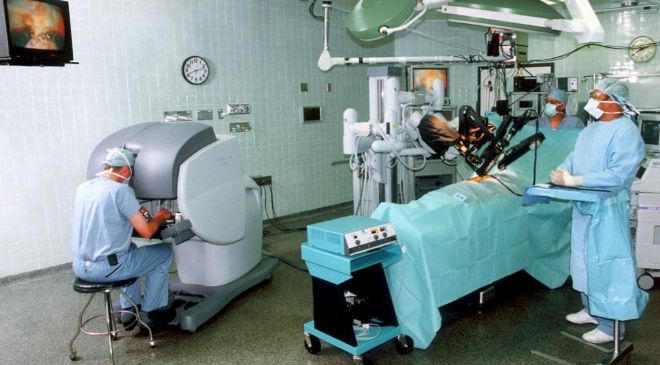
\includegraphics[width=0.8\textwidth]{figures/sistemadavinci.jpg}
		\caption{Sistema Da Vinci}
		\label{fig.sistemadavinci}
		\end{center}
\end{figure}
\item Industria: Probablemente se trate del sector donde más extendido este el uso de la robótica, desde mover una pieza de posición hasta cargar y descargar el maquinas. Sin embargo, hay una industria donde sobresale por encima del resto: el sector del automóvil. En España, según datos de la Asociación Española de Robótica, seis de cada diez robots pertenecen a este sector. Los robots se encargan de distribuir por toda una fabrica los componentes necesarios, así como posteriormente montarlos. Gracias a la robotización de la industrias, la producción ha aumentado en los últimos años de manera significativa, disminuyendo costes y errores.
\begin{figure}[H]
  \begin{center}
    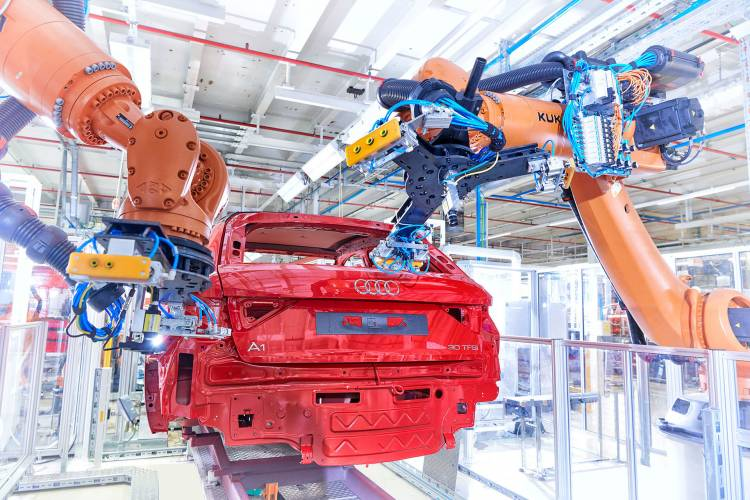
\includegraphics[width=0.8\textwidth]{figures/robotautomovil.jpg}
		\caption{Fábrica de Seat en Martorell}
		\label{fig.robotautomovil}
		\end{center}
\end{figure}
\item Militar: Si la industria es el sector donde más se utiliza la robótica, sin lugar a duda el sector militar es donde más dinero se invierte y se investiga. Actualmente hay multitud de robots usados militarmente como los vehículos aéreos no tripulados Hermes y Predator, el Goalkeeper CIWS, que es un sistema de armamento defensivo por proximidad holandés, o Samsung SGR-A1, que es un robot centinela utilizado para la vigilancia de la zona desmilitarizada entre Corea del Sur y Corea del Norte. Sin embargo, actualmente la investigación esta centrada en la elaboración de un robot humanoide capaz de caminar por terrenos irregulares y zonas catastróficas para realizar tareas de rescate y ayuda humanitaria. En este sentido, entre el año 2012 y 2015, el Departamento de Defensa de Estados Unidos, a través de su Agencia de Proyectos  de Investigación Avanzada en Defensa (DARPA)., creó una competición con el objetivo de desarrollar robots terrestres semiautónomos capaces de realizar tareas complejas en entornos peligrosos y degradados \footnote{\url{https://www.darpa.mil/program/darpa-robotics-challenge}}. El premio fue ganado por el robot humanoide desarrollado por el Instituto Avanzado de Ciencia y Tecnología de Corea, ``DRC-Hubo''.
\begin{figure}[H]
  \begin{center}
    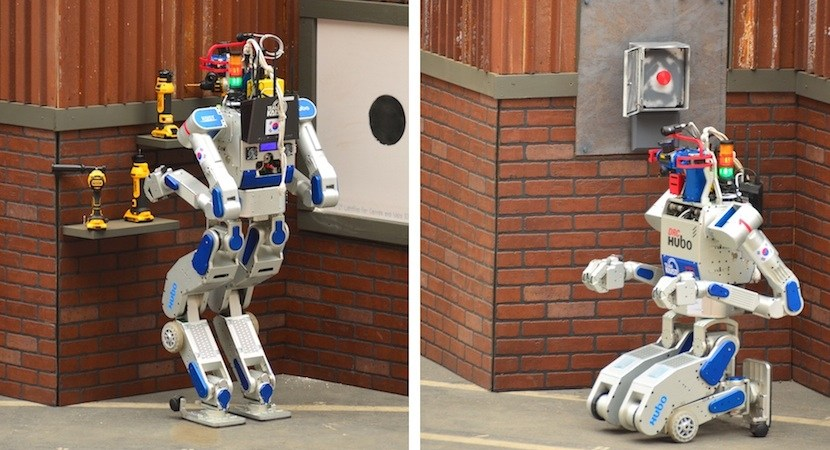
\includegraphics[width=0.8\textwidth]{figures/drchubo.jpg}
		\caption{Robot DRC-Hubo durante el DARPA Robotics Challenge}
		\label{fig.drchubo}
		\end{center}
\end{figure}
\end{itemize}

\subsection{Software para el desarrollo de componentes robóticos}

El software es el encargado de proporcionar al robot la inteligencia y autonomía necesaria para que realice las funciones o acciones que deseamos. Para facilitar esta tarea, se han creado middleware y bibliotecas especificas.

\subsubsection{Middleware}

Un robot es un sistema complejo ya que es un conjunto de diferentes componentes hardware y software (sensores, actuadores, etc.). Para cada robot, sería necesario un software personalizado que sea capaz de: leer y extraer la información necesaria de cada uno de los sensores, calcular y enviar las secuencias de acciones para que realice una determinada tarea o acción, controlar los actuadores, etc. Desarrollar este software se vuelve una tarea compleja e inútil dado que por lo general, si cambiáramos de robot este software no funcionaría de manera correcta.
En este escenario es donde un middleware nos proporcionará las herramientas que necesitamos para facilitar en gran medida la labor, ya que nos permitirá estructurar el software separando las diferentes tares (lectura de sensores, extracción de datos, especificar la velocidad, etc.) y haciendo exportable el uso de este software con cualquier otro sistema robótico al tener un marco común de comunicación gracias al middleware.
Actualmente hay una gran cantidad de middleware que permiten esta abstracción, siendo algunos de los más destacados los que señalo a continuación:
\begin{itemize}
	\item Robot Operating System (ROS)\footnote{\url{http://www.ros.org/}}: Pese a ser un middleware, se podría decir que ROS pretende ser algo más. Nos provee de la funcionalidad que cabría esperar de un sistema operativo (abstracción del hardware, control de dispositivos de bajo nivel, la trasferencia de mensajes entre procesos, administración de paquetes, etc.). El principal objetivo es permitir la reutilización del código en la investigación y desarrollo de robótica, lanzando paquetes de software que están listos para ser usados por cualquier desarrollador. ROS cuenta con una gran comunidad de colaboradores, que comparten sus paquetes y proyectos, gracias a su sitio web y repositorios.
	\item Internet Communication Engine (ICE) \footnote{\url{https://zeroc.com/}}: Creado por la empresa ZeroC, se trata de un middleware orientado a objetos que permite la creación de aplicaciones multilenguaje y multiplataforma, permitiendo la comunicación con diferentes arquitecturas de red (UDP, TCP, WebSockets, etc.). ICE no es un middleware robótico propiamente dicho, pero su uso facilita el desarrollo de la conectividad con sistemas robóticos, al permitirnos crear nuestras propias interfaces para el intercambio de datos.
	\item Open Robot Control Software project (Orocos) \footnote{\url{http://www.orocos.org/}}: Se trata de un proyecto de software libre cuyo objetivo es la creación de un paquete de software para el control de robots.
	\item Orca \footnote{\url{https://www.orcaconfig.com/}}: Se trata de un middleware de código libre que se originó a partir del proyecto Orocos. Orca está diseñado para desarrollar sistemas robóticos basados en componentes. Su principal objetivo es permitir, facilitar y simplificar la reutilización del código entre desarrolladores.
	\item Middleware for Robots (Miro): Se trata de un middleware orientado a objetos para el control de robots móviles, y basado en CORBA (Common Object Request Broker Architecture). El hecho de que sea orientado a objetos permite la interoperabilidad entre procesos y plataformas cruzadas para el control de robots distribuidos.
	\item JdeRobot \footnote{\url{https://jderobot.org/}}: Se trata de una plataforma de código abierto para el desarrollo de aplicaciones de visión artificial y robóticas, compatible con middlewares de comunicación ICE y ROS y desarrolladas principalmente en Python y C++.
\end{itemize}

\subsubsection{Bibliotecas}

En programación, una biblioteca es una colección de recursos utilizados para el desarrollo de software. Hay multitud de bibliotecas para el desarrollo de sistemas robóticos: bibliotecas para procesar imágenes, interactuar con el robot, procesar elementos 3D, etc. Las bibliotecas más utilizadas son:
\begin{itemize}
	\item OpenCV \footnote{\url{https://opencv.org/}}: Es la biblioteca de visión artificial por excelencia. Creada originalmente por Intel, es de código abierto y desarrollada en C++. Actualmente dispone de interfaces en C++, C, Python, Java y están empezando a desarrollar para JavaScript.
	\item Point Cloud Library (PCL) \footnote{\url{http://pointclouds.org/}}: Se trata de una biblioteca de código abierto que proporciona algoritmos para el procesamiento de nubes de puntos y geometría 3D.
	\item Bibliotecas de ROS: ROS proporciona bibliotecas para cada lenguaje de programación al que da soporte, ofreciendo una serie de funciones y algoritmos que nos permite crear aplicaciones que interactúan rápidamente con ROS. Las bibliotecas más utilizadas son rospy \footnote{\url{http://wiki.ros.org/rospy}}, que está desarrollada para Python y roscpp \footnote{\url{http://wiki.ros.org/roscpp}}, que está desarrollada para ser usada con C++. Cabe destacada, también, la biblioteca roslibjs, que ofrece las funcionalidades para JavaScript.
\end{itemize}

\subsubsection{Simuladores}

Un simulador robótico nos permite imitar el funcionamiento de un sistema robótico para poder probar las aplicaciones, evitando que surjan fallos críticos a la hora de hacerlo funcionar con el sistema real. Estos fallos pueden conllevar averías muy costosas a nivel monetario y de tiempo, que conllevarían retrasos importantes a la hora de realizar el desarrollo. Los simuladores más utilizados son:
\begin{itemize}
	\item Gazebo \footnote{\url{http://gazebosim.org/}}: Se trata de uno de los simuladores más utilizados en la actualizada gracias a su fácil manejo y su intuitiva interface. Gazebo es un simulador de código abierto que ofrece múltiples motores de físicas, motores de renderizado avanzado, soporte para plug-ins y programación en la nube. Además, dispone de un gran número de robots, sensores y cámaras para simular, lo que permite realizar las pruebas de nuestras aplicaciones de forma bastante realista y, así poder utilizar nuestra aplicación con el sistema físico sin miedo a que sufra daños.
	\item ROS Development Studio (RDS \footnote{\url{http://www.theconstructsim.com/}}): Elaborado por la empresa española TheConstruct, se trata de un simulador web que permite simulador sistemas robóticos, a la vez que ofrece un editor y una consola para poder crear nuestro código, pero únicamente ofrece soporte para Python gracias a Jupyter. La gran ventaja que ofrece este simulador es que no es necesario realizar ninguna instalación, simplemente registrarte en su página web y acceder con un navegador. Ofrecen desde una versión básica gratuita hasta una versión para expertos con una tarifa mensual.
\end{itemize}
Existen otros simuladores como son Stage para la simulación en 2D o  Webots, pero no tan utilizados como Gazebo o sin las ventajas de RDS.

\section{Tecnologías web}
Desde que en el año 1992, Tim Berners-Lee ideara y desarrollara las primeras herramientas para facilitar compartir información entre los científicos del CERN desde cualquier parte del mundo, dando lugar a la posteriormente llamada World Wide Web o como se conoce coloquialmente la web, ha sufrido una gran evolución, consiguiendo que la sociedad actual no se pueda entender sin la existencia de la misma. Sin embargo, pese a la gran evolución, el propósito de la web no ha cambiado, es decir, que acceder a la información sea lo más fácil posible. Sí lo ha hecho la manera en que la utilizamos. La aparición de aplicaciones web como las redes sociales, los servicios de streaming o los comercios electrónicos, han supuesto un impulso importante en el uso de la web y, por consiguiente, la necesidad de idear nuevas herramientas que faciliten el desarrollo de webs.

\subsection{Arquitectura de una aplicación web}
Desde su creación, el modelo para que un sitio o aplicación web funcione no ha variado.
\begin{itemize}
	\item Cliente: Realiza las peticiones de recursos a diferentes servidores web a través de un localizador uniforme de recursos (URL). Generalmente, la función de cliente la realizada un navegador.
	\item Servidor: Almacena la información de la aplicación web y sirve los contenidos acorde a las peticiones realizadas por el navegador.
	\item Http: Es el protocolo creado por Bernens-Lee que permite el intercambio de información entre el cliente y el servidor.
\end{itemize}
\begin{figure}[H]
  \begin{center}
    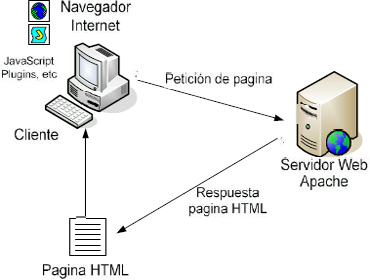
\includegraphics[width=0.8\textwidth]{figures/arquitecturaweb.jpg}
		\caption{Arquitectura de una aplicación web}
		\label{fig.arquitecturaweb}
		\end{center}
\end{figure}

\subsection{Tecnologías del lado del cliente}
Estas tecnologías son las encargadas de dar forma a la interfaz de usuario y de establecer la comunicación con el servidor. El navegador es capaz de leer e interpretar estas tecnologías. Las más utilizadas son las siguientes:
\begin{itemize}
	\item Hyper-Text Markup Lenguage (HTML): Es el lenguaje de descripción de aplicaciones web que nos permite especificar las características visuales.
	\item Hojas de estilo en cascada (CSS): Es el lenguaje utilizado para describir la presentación semántica (el aspecto y el formato) de un documento en lenguaje de marcas.
	\item JavaScript: Es un lenguaje de script orientado a objetos y guiado por eventos que nos permiten realizar acciones en el cliente e interactuar con el servidor u otras aplicaciones web.
\end{itemize}

\subsection{Tecnologías del lado del servidor}
Estas tecnologías son las encargadas de dar forma al servidor web de manera que permita el acceso a bases de datos, conexiones de red, recursos compartidos, en definitiva, se encarga de realizar todas las tareas necesarias para crear la aplicación web que se visualizará en el cliente. Las tecnologías más utilizadas son las siguientes:
\begin{itemize}
	\item Common Gatewey Interface (CGI): Fue de las primeras tecnologías del lado del servidor en aparecer, se creó inicialmente para gestionar formularios. No se trata de un lenguaje de programación sino  de un mecanismo de comunicación entre el cliente y un programa externo, que proporcionará el contenido de la aplicación web. Actualmente se utiliza una variante llamada Fast-CGI que proporciona una mayor rapidez.
	\item PHP: Creado en 1994, es la tecnología más utilizada. Se trata de un lenguaje de programación de uso general de script que originalmente fue diseñado para proporcionar contenido web dinámico. Su código está empotrado en el código HTML y es interpretado por un servidor web para generar la aplicación web, evitando la necesidad de acceder a un archivo externo.
	\item Servlets: Son programas escritos en Java que se ejecutan sobre un servidor de aplicaciones mediante la maquina virtual de Java (JVM). Estos programas (servlets) son ejecutados por el servidor para manejar cada una de las peticiones del cliente. Se trata de una tecnología con un concepto similar a CGI, pero beneficiándose de las ventajas de el entorno Java.
	\item JavaServer Pages (JSP):Se trata de una tecnología Java que permite generar contenido web dinámico en forma de documentos HTML. El código Java, a diferencia que en los Servlets, va incrustado en el HTML y se compila dinámicamente como un servlet.
	\item Active Server Page (ASP): Creado por Microsoft en 1996. Se trata de código que se ejecuta en el servidor y genera un archivo HTML que devuelve al cliente. Al ser una tecnología creada por Microsoft, permite la compatibilidad con componentes ActiveX (acceso a base de datos, scripts, etc.) lo que proporciona una gran potencia y flexibilidad. Esta tecnología solo puede ser utilizada en servidores con sistemas operativos de Microsoft.
	\item Python, Django: Se trata de un framework programado en Python que proporciona un conjunto de componentes en el lado del servidor para ayudar a la hora de desarrollar una aplicación web. Sigue el diseño de Modelo-Vista-Controlador, que se trata de un modelo que separa la lógica y datos de la interfaz gráfica y de las comunicaciones y eventos. Cuando un cliente solicita una URL al servidor, esta pasa por Django que analizará la URL solicitada y pasará la petición a la función correspondiente llamada vista. En esta función se ejecutará lo necesario para proporcionar al cliente lo solicitado con su URL.
	\item Ruby on Rails: Al igual que Django, Ruby on Rails se trata de un framework para facilitar el desarrollador web programado en Ruby que sigue el diseño de Modelo-Vista-Controlador. El funcionamiento de Django y Rails es muy similar, siendo la principal diferencia el lenguaje en el que están programados, siendo necesario menos código en el caso de Rails.
	\item Node.js: Se trata de un entorno de ejecución multiplataforma de código abierto para el lado del servidor basándose en el lenguaje JavaScript. Este entorno se basa en eventos y gestiona todas las operaciones con una programación asíncrona. Todo esto facilita el desarrollo de aplicaciones web escalables de manera sencilla y con robustas.
\end{itemize}

\subsection{Tecnologías web en la actualidad}
Actualmente, el uso de tecnologías web está muy extendido, no concibiendo la vida moderna sin ellas. Las redes sociales, tiendas online, servicios de streaming, etc, son utilizados en multitud de ocasiones a lo largo de nuestro día a día. A continuación se mostrará algunos ejemplos de aplicaciones y paginas web más utilizadas:
\begin{itemize}
\item Spotify\footnote{\url{https://www.spotify.com/es/}}: Aplicación creada para la reproducción de música vía streaming, actualmente cuenta con más de 75 millones de usuarios activos convirtiéndose en una de las principales formas de escuchar música en la actualidad. La aplicación esta desarrollada mediante JavaScript (lado del cliente) y Python (lado del servidor).
\item Facebook\footnote{\url{https://es-es.facebook.com/}}: Se trata de la red social más conocida y que provoco el auge de las mismas, actualmente cuenta con más de 2200 millones de usuarios. Originalmente nació como una página web desarrollada mediante HTML y JavaScript para el lado del cliente y PHP para el lado del servidor, ha evolucionado hasta disponer una aplicación que puede ser utilizada en nuestros teléfonos móviles.
\item Google maps\footnote{\url{https://www.google.es/maps}}: Se trata de un servicio de mapas que permite desplazarse por el mundo, ver fotografías por satélite o recorrer una ubicación a pie de calle. Actualmente es utilizada para indicar ubicaciones, a modo de GPS o para encontrar lugares de interés, convirtiéndose en un sistema de referencia en la sociedad de hoy en día ya que se envían ubicaciones a través de esta aplicación de manera constante. La base de esta aplicación es JavaScript, usando HTML y CSS para la interfaz gráfica.
\item YouTube\footnote{\url{https://www.youtube.com/}}: Aplicación y página web dedicado a la compartición de videos entre usuarios. Actualmente, cuenta con más de 1900 millones de usuarios al mes y cada minuto se suben más de 120 horas de vídeo, llegando a convertirse en un oficio para miles de personas que ganan dinero publicando sus propios videos comentando videojuegos, consejos o criticas de multitud de cosas (móviles, películas, juguetes, etc.). YouTube está desarrollado mediante JavaScript y HTML en el lado del cliente y Python en el lado del servidor, incluso proporciono el primer reproductor de video incrustado en el HTML, que posteriormente fue incluido por el World Wide Web Consortium.
\item Whatsapp\footnote{\url{https://www.whatsapp.com/}}: Es una aplicación de mensajería instantánea que permite el intercambio entre usuario de mensajes a través de internet sin coste adicional. Cuenta con más de mil millones de usuario actualmente, ha supuesto una revolución al provocar la extinción del servicio de mensajes cortos (SMS) que conllevaban un coste mensual alto en beneficio de las operadoras móviles. Tras ser usado como aplicación, en el año 2015 se lanzó la versión web de Whatsapp para su usó en un ordenador, provocando que la aplicación de mensajería de Google, Hangouts, sufriera una reducción importante de usuarios, siendo uno de los factores que ha llevado a Google a anunciar el cierre del servicio en el año 2020.
\end{itemize}

\section{Tecnologías web en robótica}

La utilización de tecnologías web en robótica es aún, pese a su aumento en los últimos tiempos, un campo con poco desarrollo. Sin embargo, debido a las ventajas que ofrece frente a otras tecnologías (el mismo código funciona en cualquier plataforma, no es necesario realizar ninguna instalación, etc.) es un campo prometedor de cara al futuro.

Como se ha mencionado anteriormente, aún no hay muchos desarrollos basados en tecnologías web, siendo el más importante de ellos las bibliotecas y herramientas de código abierto para su utilización con el middleware ROS, elaboradas por la comunidad de Robot Web Tools \footnote{\url{http://robotwebtools.org/}}.
Los desarrollos más importantes que han realizado son:
\begin{itemize}
	\item Rosbridge Suite: Proporciona una interfaz usando JSON para ROS que permite a cualquier cliente enviar JSON para conectarnos con el robot, mediante las capas de comunicación WebSockets, UDP y TCP. Realmente podría entenderse como un servidor intermedio que recibe o envía la información a un cliente web.
	\item roslibjs: Se trata de la biblioteca que da soporte a la interactuación entre una aplicación web desarrollada en JavaScript con ROS. 
	\item ros2djs y ros3djs: Son las bibliotecas elaboradas para gestionar la visualización de elementos en dos y tres dimensiones, respectivamente. Están elaboradas utilizando roslibjs y proporcionan funciones que son estándares en ROS como la elaboración de mapas, el procesado de nubes de puntos o del escaneo laser.
\end{itemize}

Adicionalmente, ofrecen una serie de herramientas como son un servidor de video web, una herramienta para mostrar e interactuar con la navegación autónoma del robot, una herramienta para la creación de teleoperadores de robots, etc.

\section{Trabajos Previos}
Una parte de este proyecto está basado en el TFG elaborado por Aitor Martínez \footnote{\url{https://jderobot.org/Aitormf-tfg}}. En este trabajó, utilizando tecnologías web, se crearon tres aplicaciones que eran capaces de conectarse con varios sistemas robóticos. El resto del proyecto se basará en la adaptación a tecnologías web del visor 3D y del servidor de imágenes desarrollados con C++ de la plataforma JdeRobot.

\subsection{CameraViewjs}

Se trata de un visualizador de imágenes, desarrollado utilizando JavaScript, HTML5 y CSS3 en el lado del Cliente y NodeJS en el lado del servidor, e ICE como middleware. Esta aplicación permite la visualización de las imágenes recibidas desde un servidor de imágenes, ya sean obtenidas desde una webcam, una cámara conectada a un robot o almacenadas en el dispositivo.

\begin{figure}[H]
  \begin{center}
    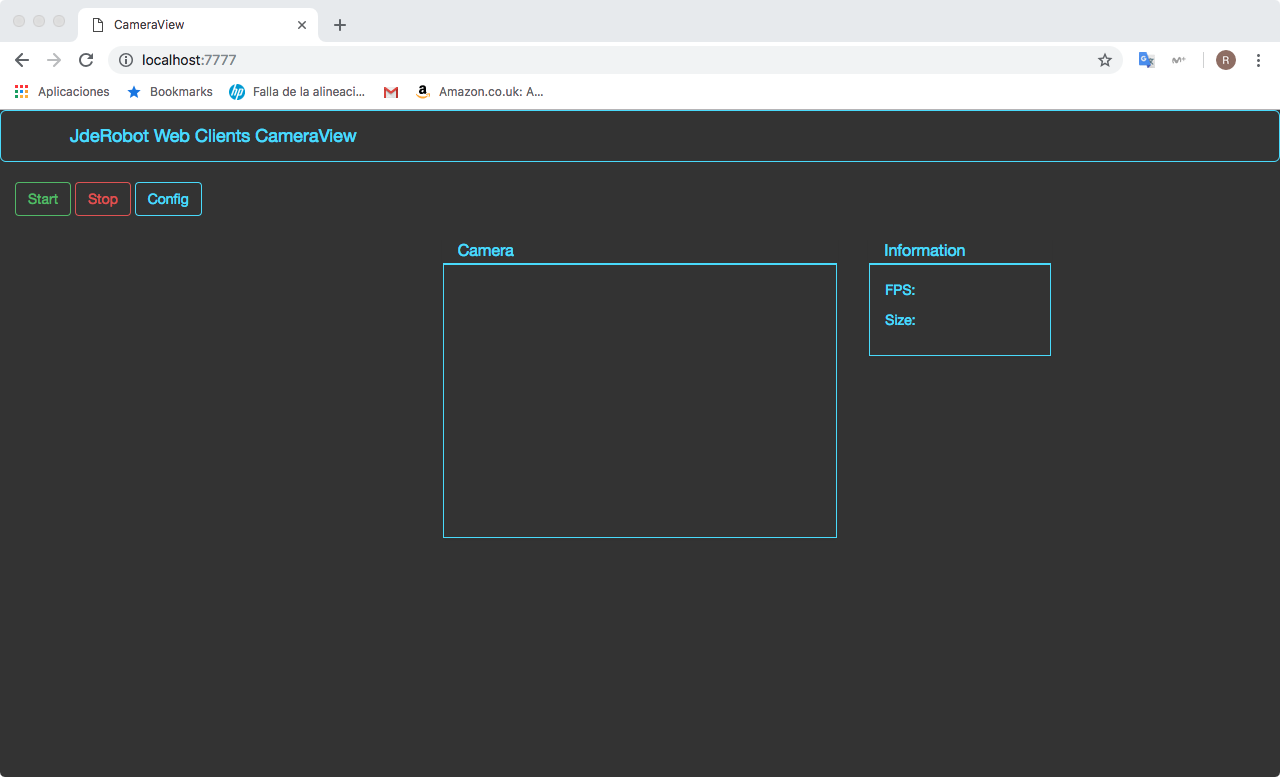
\includegraphics[width=0.8\textwidth]{figures/cameraviewjs.png}
		\caption{CameraViewjs}
		\label{fig.cameraviewjs}
		\end{center}
\end{figure}

\subsection{KobukiViewerjs}

Se trata de un visualizador y teleoperador de robots del tipo Turtlebot, desarrollado utilizando JavaScript, HTML5 y CSS3 en el lado del Cliente y NodeJS en el lado del servidor, e ICE como middleware. Consta de varias partes, la primera de ellas es mostrar las imágenes obtenida a través de las dos cámaras de las que dispone el robot (izquierda y derecha), otra parte donde muestra la imagen del escaneo láser obtenida, una representación tridimensional del robot y el movimiento del mismo, y por último, el teleoperador, que envía al robot una velocidad lineal y otra angular para indicar tanto el movimiento en linear recta como la orientación del mismo.

\begin{figure}[H]
  \begin{center}
    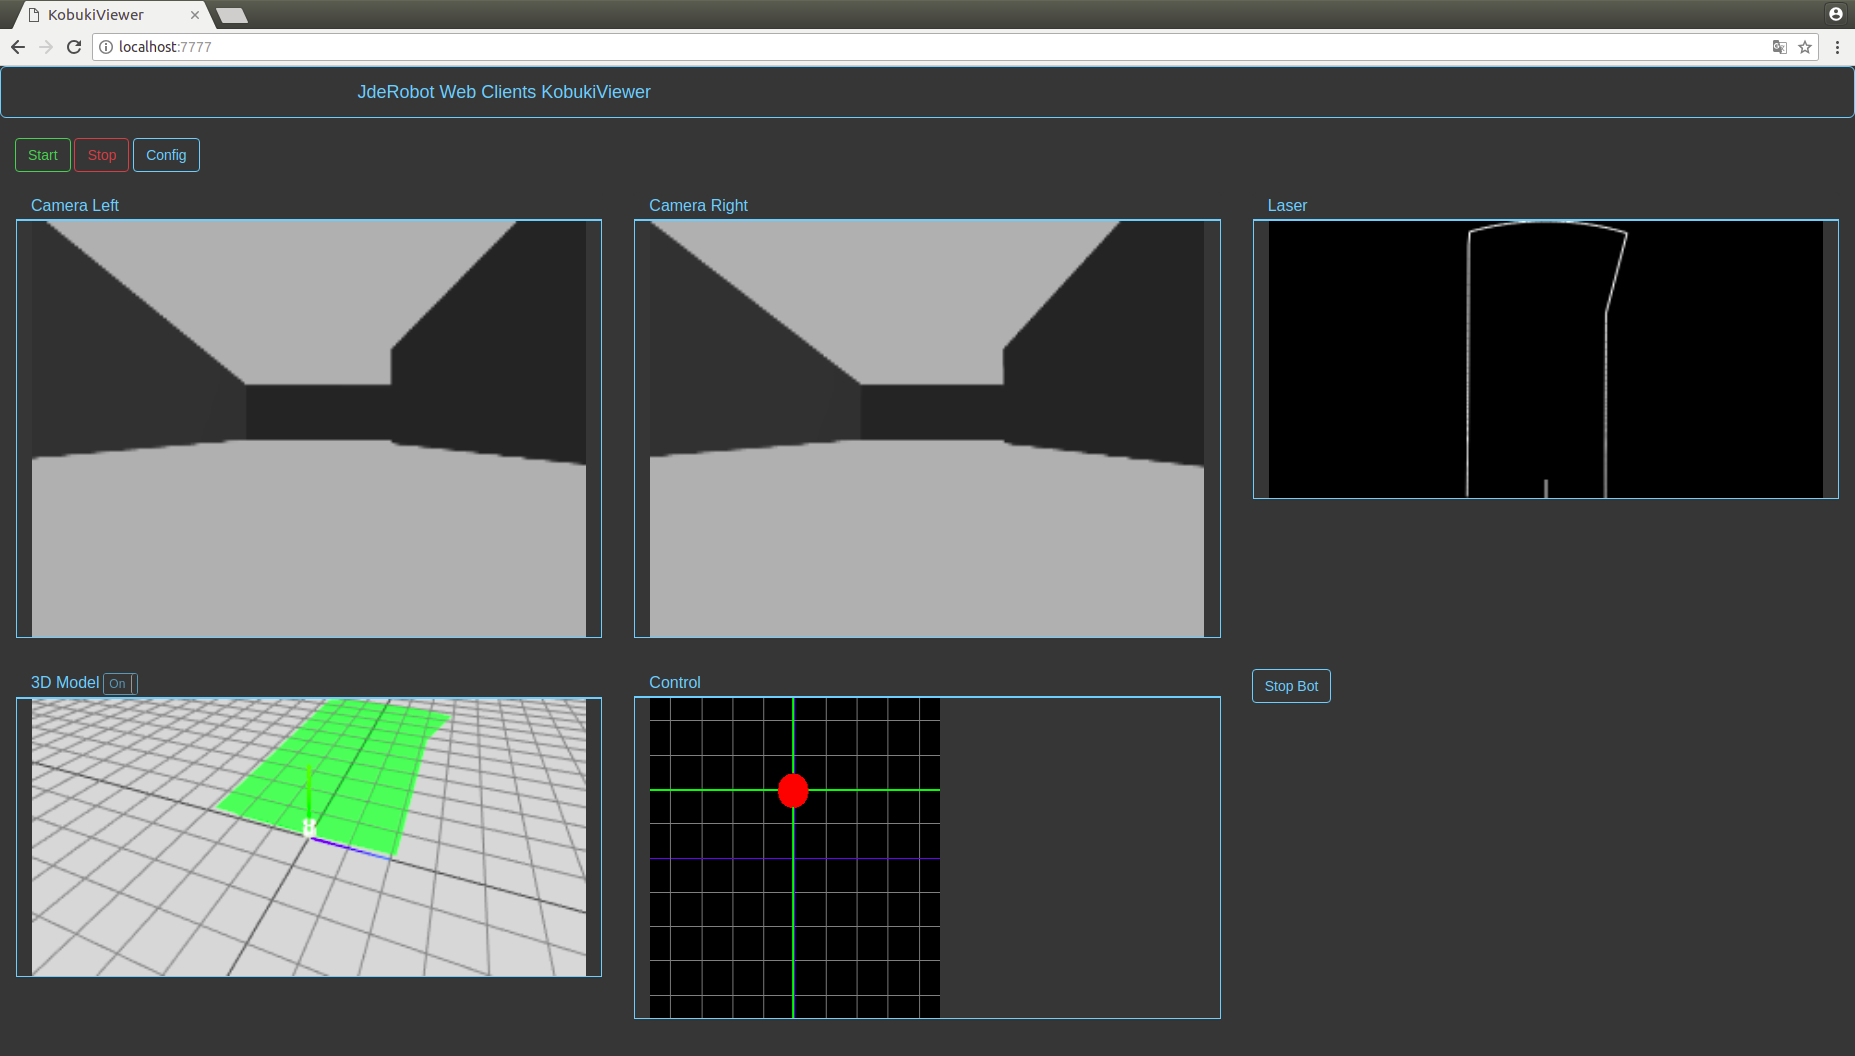
\includegraphics[width=0.8\textwidth]{figures/kobukiviewerjs.png}
		\caption{KobukiViewerjs}
		\label{fig.kobukiviewerjs}
		\end{center}
\end{figure}

\subsection{UavViewerjs}

Se trata de un visualizador y teleoperador de drones, desarrollado utilizando JavaScript, HTML5 y CSS3 en el lado del Cliente y NodeJS en el lado del servidor, e ICE como middleware. La aplicación tiene integrada sobre la misma pantalla el teleoperador y la imagen obtenida de la cámara, pudiéndose elegir si deseamos mostrar la cámara frontal o de abajo del dron. Consta también de una representación tridimensional del dron y de su movimiento. Desde la aplicación se teleopera mediante él envió de una velocidad lineal y otra angular, además se le indica cuando se desea aterrizar y despegar.

\begin{figure}[H]
  \begin{center}
    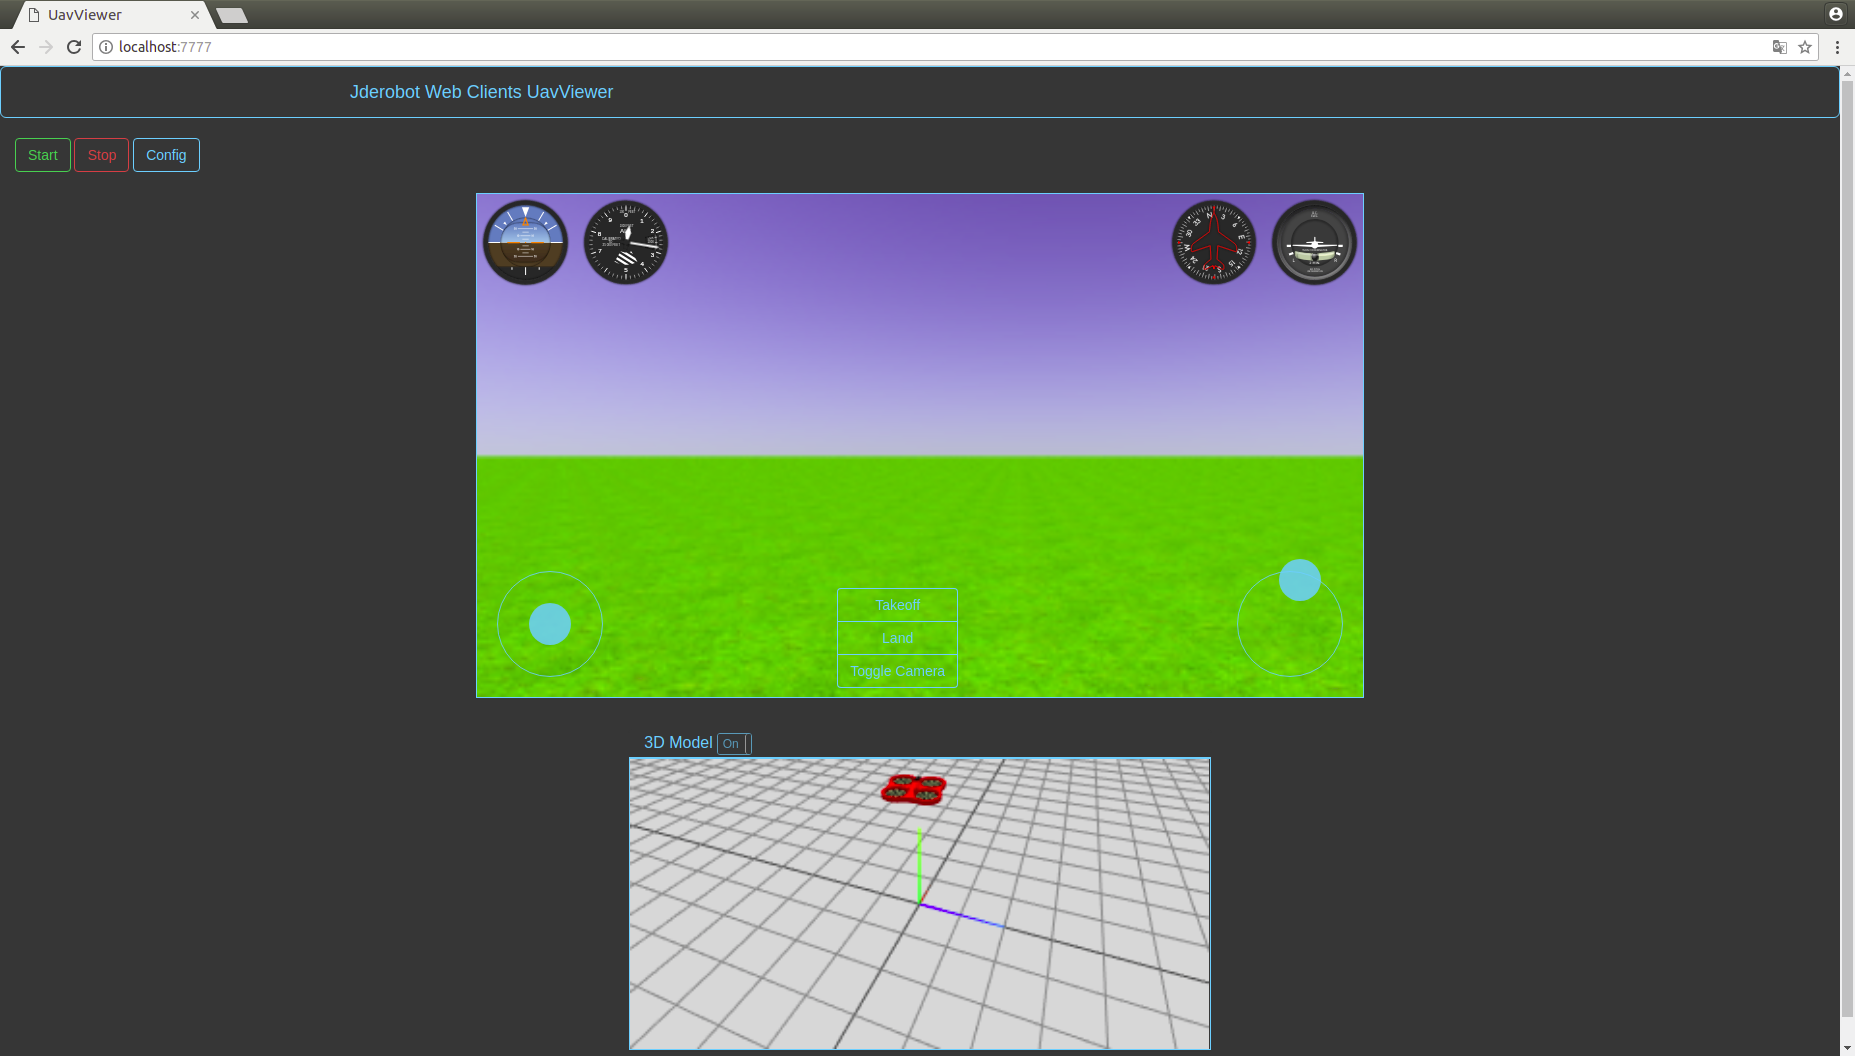
\includegraphics[width=0.8\textwidth]{figures/uavviewerjs.png}
		\caption{UavViewerjs}
		\label{fig.uavviewerjs}
		\end{center}
\end{figure}

\subsection{3DViewer}
3DViewer \footnote{\url{https://jderobot.org/Tools}} es la herramienta para visualizar puntos 3D de la plataforma JdeRobot. Este visor es utilizado conjuntamente con la práctica de JdeRobot Academy de reconstrucción 3D \footnote{\url{https://jderobot.org/JdeRobot-Academy}} para reconstruir mediante puntos de la imagen obtenida con un par de cámaras RGB.

\begin{figure}[H]
  \begin{center}
    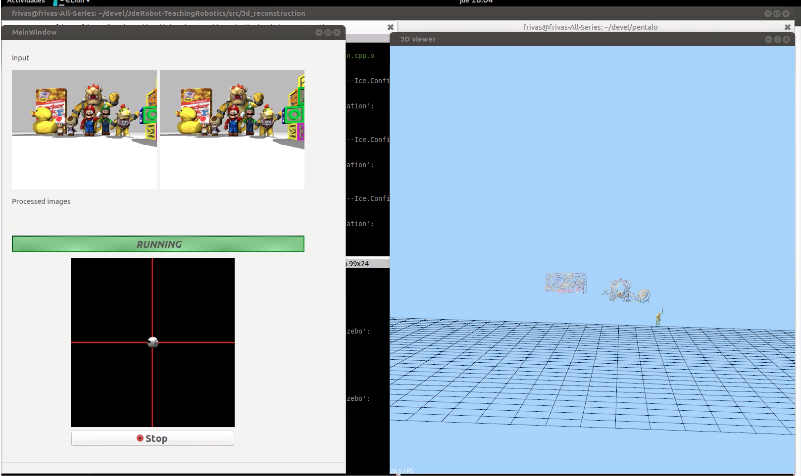
\includegraphics[width=0.8\textwidth]{figures/3DViewer.png}
		\caption{3DViewer usado con la práctica de JdeRobot Academy}
		\label{fig.3DViewer}
		\end{center}
\end{figure}
\subsection{Cameraserver}
Cameraserver \footnote{\url{https://jderobot.org/Handbook}} es el componente de la plataforma JdeRobot que sirve las imágenes obtenidas a través de una fuente de video, real o simulada, y transmitidas mediante del middleware ICE para su visualización por parte de uno o varios clientes.

\lhead[]{CAP\'ITULO \thechapter. OBJETIVOS}
\chapter{Objetivos}\label{cap.objetivos}
En este capitulo se presentaran los objetivos planteados para este proyecto, los requisitos marcados y la metodología utilizada para alcanzarlos.

\section{Objetivos}
La principal meta de este trabajo es la de enriquecer con tecnologías web las herramientas robóticas existentes en la plataforma JdeRobot. Para alcanzar este objetivo, se ha dividido el trabajo en tres partes: 
\begin{itemize}
\item Modificar los tres visores elaboradas mediante tecnologías web existentes en la plataforma JdeRobot, CameraViewjs, KobukiViewerjs y UavViewerjs, para su utilización con el middleware ROS, además de ICE como hasta ahora.
\item Elaborar un nuevo driver robótico utilizando tecnologías web, cuyo cometido sera el de servidor de imágenes a los distintos visores existentes en JdeRobot. 
\item Creación mediante tecnologías web, de un nuevo visor, que permitirá la visualización de elementos 3D (puntos, líneas y modelos 3D) que utilizara como middleware de comunicación, ICE.
\end{itemize}
Además, se ha utilizado el framework Electron en todos ellos para posibilitar que, además de usando un navegador, se puedan ejecutar como si de una aplicación de escritorio se tratase.

\section{Requisitos}
Los requisitos que se han tenido en cuenta a la hora de desarrollar todo el software de este trabajo han sido los siguientes:
\begin{itemize}
\item El sistema operativo utilizado ha sido Ubuntu 16.04 LTS y macOS HighSierra, además, gracias a utilizar tecnologías web, todos los componentes pueden ser ejecutados en cualquier sistema operativo.
\item Se ha utilizado la versión de NodeJS 8.9.1 y de NPM 6.4.0.
\item Los middleware utilizados han sido JdeRobot en su versión 5.6.4, ROS en su versión Kinetic y ICE en su versión 3.6.4.
\item Para permitir ejecutar la ejecución de todo los elementos como una aplicación de escritorio, se ha utilizado Electron en la versión 1.8.
\item Se ha utilizado HTML5, CSS3 y JavaScript para la elaboración de los software.
\item El funcionamiento con el middleware ROS sera mediante la biblioteca Rosbridge Server de RobotWebTools.
\end{itemize}

\section{Metodología}
La metodología elegida para la ejecución del trabajo ha sido el desarrollo en espiral. Se trata de uno de los modelos más utilizados en el desarrollo de software, y consiste en la realización de una serie de cilcos o iteraciones que se repiten en forma de espiral.
\begin{figure}[H]
  \begin{center}
    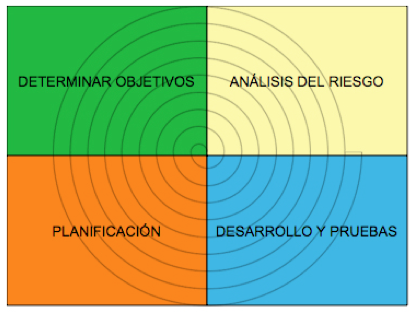
\includegraphics[width=0.8\textwidth]{figures/desarrolloespiral.png}
		\caption{Modelo de desarrollo en espiral}
		\label{fig.desarrolloespiral}
		\end{center}
\end{figure}
Cada iteración o ciclo esta formado por cuatro etapas.
\begin{enumerate}
\item Determinación de los objetivos a alcanzar para que el ciclo sea finalizado de manera exitosa.
\item Analizar los riegos que conlleva las elecciones tomadas para realizar el desarrollo, y establecer alternativas para solventar los posibles inconvenientes.
\item Desarrollar y probar los objetivos establecidos en la primera fase.
\item Planificar las siguientes etapas del proyecto, teniendo en cuenta los resultados obtenidos en esta interacción.
\end{enumerate}
De cara a poder llevar un mejor control del trabajo, se han tenido reuniones semanales con el tutor, en las que se marcaban los objetivos para la siguiente semana, se exponían dudas o posibles problemas  así como se establecen posibles alternativas, y se revisaba el trabajo previo. Con estas reuniones semanales se consigue tener flujo de trabajo constante y fluido, disminuyendo la posibilidad de quedar bloqueado en algún punto durante un largo periodo de tiempo.

Además, se ha elaborado un bitácora en la mediawiki\footnote{\url{https://jderobot.org/Rperez-tfg}} de JdeRobot, donde quede reflejado todos los progresos así como videos demostrativos de los avances. También se dispone de un repositorio en github\footnote{\url{https://github.com/RoboticsURJC-students/2017-tfg-roberto-perez}} donde se ha ido subiendo todo el código para su verificación y prueba por personas externas.

\section{Plan de Trabajo}
De cara a cumplir los objetivos marcados y enfocar mejor los posibles problemas y sus posibles soluciones, lo primero que se ha realizado es una familiarización con el entorno de trabajo.

\begin{enumerate}
\item Comprender el funcionamiento de Electron y realización de pequeñas pruebas para aprender a usarlo.
\item Familiarización con el entorno JdeRobot y Gazebo.
\item Comprender el funcionamiento de los visores existentes desarrollados en tecnologías web (CameraViewjs, KobukiViewerjs y UavViewerjs) y ejecutarlos para analizar su funcionamiento.
\item Realizar las modificaciones para que funcionen con el framework Electron.
\item Comprender el funcionamiento de los middleware ICE y ROS, realizando pequeñas pruebas.
\item Modificación de los visores para que funciones tanto con ICE (como hasta ahora), como con ROS.
\item Creación de nuevo driver para servir imágenes con el middleware ROS.
\item Comprender el funcionamiento del visor 3D existente en la plataforma JdeRobot desarrollado en C++, así como su conectividad con la práctica de Reconstrucción 3D de JdeRobot Academy.
\item Elaboración del visor 3D con tecnologías web y el middleware ICE para que muestre puntos y se conecte con los elementos de la práctica de Reconstrucción 3D.
\item Ampliación del visor 3D para que además de los puntos, muestre también segmentos y modelos 3D enviados por un cliente escrito en cualquier lenguaje de programación.
\end{enumerate}



\lhead[]{CAP\'ITULO \thechapter. INFRAESTRUCTURA}
\chapter{Infraestructura}\label{cap.infraestructura}
En este capitulo se describirán las tecnologías sobre las que se cimienta este trabajo. Para empezar, se detallará el funcionamiento del framework Electron y Node.js, ya que todo el desarrollo de este trabajo será compatible con él. Se profundizará en los dos middleware utilizados, ICE y ROS, y en el entorno JdeRobot. Para finalizar, se describirá el API para el renderizado de gráficos WebGL, concretamente la biblioteca Three.js, y WebRTC para la conexión con los elementos multimedia.

\section{La plataforma JdeRobot}
JdeRobot \footnote{\url{https://jderobot.org/Main_Page}} es el framework de software libre para el desarrollo de robótica y visión artificial creado por el grupo de robótica de la Universidad Rey Juan Carlos y licenciado bajo GPL v3 \footnote{\url{http://www.gnu.org/licenses/gpl-3.0-standalone.html}}. Su desarrollo principalmente está realizado mediante C, C++ y Python, incorporando desarrollo en JavaScript como el tratado en este trabajo.

JdeRobot está basado en componentes que son interconectados mediante el uso de middlewares como ICE o ROS, facilitando el acceso a los dispositivos hardware. Estos componentes obtienen mediciones  de los sensores u ordenes del motor a través de llamadas a funciones locales. JdeRobot conecta esas llamadas a drivers conectados a sensores (para la recepción de las mediciones) o actuadores (para las ordenes), ya sean reales o simulados. Estas funciones locales forman la API de la capa de abstracción. La plataforma también ofrece una serie de herramientas para facilitar la teleoperación o el tratamiento de las mediciones de los sensores, y bibliotecas.

Para el desarrollo de este proyecto, se usará la versión de JdeRobot 5.6.4

\section{El Middleware ICE}
Se trata de un Framework orientado a objetos que ayuda a crear aplicaciones distribuidas fácilmente. ICE se ocupa de todas las interacciones con las interfaces de programación de bajo nivel de red (inhibe al desarrollador de la tarea de apertura de puertos, conexiones de red o serialización de datos). El objetivo principal de ICE es facilitar su uso y el desarrollo de aplicaciones, de modo que en muy poco tiempo se pueda aprender a utilizarlo.

\begin{figure}[H]
  \begin{center}
    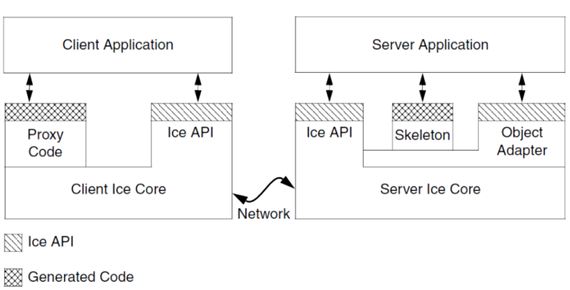
\includegraphics[width=0.8\textwidth]{figures/estructuraice.png}
		\caption{Estructura de Cliente - Servidor con Ice}
		\label{fig.estructurarice}
		\end{center}
\end{figure}

ICE tiene un lenguaje de especificación propio llamado Slice (Specification Language for ICE) que nos permite la abstracción fundamental para separar interfaces de objetos de sus implementaciones. Este lenguaje especifica las interfaces, operaciones y tipos de parámetros utilizados por la aplicación. Cada una de las aplicaciones que queramos que interaccionen entre sí, deben compartir la misma descripción Slice. Esta descripción es independiente del lenguaje en el que está desarrollada nuestro cliente o servidor de modo que sea posible su utilización con clientes y servidores escritos en diferentes lenguajes de programación.

Las interfaces Slice podrían verse como un contrato firmado entre un cliente y un servidor para compartir los mismos tipos, funciones y elementos, dando igual el lenguaje de programación en el que estén escritos, ya que posteriormente se compilan usando el compilador correspondiente al lenguaje de programación correspondiente. Si el cliente y el servidor no compartiesen la misma interface slice, la conexión no podría llevarse a cabo al no conocer las funciones o tipos que maneja cada uno.

Para este trabajo se va a utilizar su versión para JavaScript, sin embargo el soporte para este lenguaje es relativamente reciente, por lo que muchas de las funcionalidades que ofrece para otros lenguajes de programación como C++ o Python, no están disponibles para JavaScript. Sobre todo este hecho es manifiesto en que no hay soporte para la creación de un servidor completo mediante JavaScript, por ello durante este trabajo se ha optado por utilizar ICE únicamente como cliente, con las ventajas e inconvenientes a los que se hará referencia en próximos capítulos.

La versión de ICE que se usará en este trabajo será la 3.6.4

\section{El Middleware ROS}
Se trata de un Framework para el desarrollo de software robótico que ofrece las funcionalidades de un sistema operativo (abstracción del hardware, control de dispositivos de bajo nivel, mantenimiento de paquetes, etc.). ROS ofrece una serie de herramientas, bibliotecas y convenciones para simplificar la tarea de crear complejos y robustos robots. Nace con la idea de fomentar el desarrollo colaborativo, es decir que cualquier persona que realice un desarrollo puede subir a los repositorios que ofrece ROS para ello, de modo que otra persona pueda utilizarlo para usarlo en su proyecto.

El elemento fundamental del funcionamiento de ROS es el nodo. Un nodo es un proceso que realiza cálculos y se comunican entre sí mediante un sistema de publicación - subscripción para conexiones asíncronas y anónimas, o servicios para las conexiones síncronas. Los nodos operan en una escala de bajo nivel, es decir cada nodo se ocupa de un parte del sistema de control de robot, por ejemplo un nodo se ocupa de los motores, otro nodo se ocupa de realizar la localización, etc. Este elemento proporciona mayor tolerancia a los fallos al ser bloques separados y aislados, y se reduce la complejidad del código.

En el sistema de comunicación asíncrona, un nodo actúa como publicador que transmite un mensaje con una etiqueta llamada topic por el canal para que sea recibido por cualquier otro nodo que se subscriba a esta etiqueta o topic. El mensaje enviado es una estructura de datos simple, que comprende campos tipados. ROS ofrece una serie de formatos de mensajes estándar que cubren la mayoría de necesidades de uso común (mensajes para sensores, cámaras, movimiento, láseres, nubes de puntos, etc).

\begin{figure}[H]
  \begin{center}
    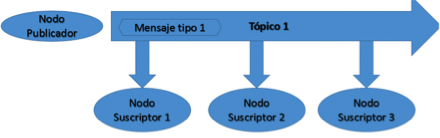
\includegraphics[width=0.8\textwidth]{figures/publicadorsubscriptor.png}
		\caption{Estructura del sistema de comunicación Publicador - Subscriptor}
		\label{fig.publicadorsubscriptor}
		\end{center}
\end{figure}

El sistema de comunicación síncrona, es el típico sistema cliente-servidor a través del cual un nodo ROS es el prestador del servicio que permanece en escucha continua y el resto de nodos le envían mensajes de solicitud. Cada servicio está definido por el tipo de servicio que define la cantidad y tipo de datos que necesita el servicio tanto para recibir como petición, como para enviar como respuesta.

\begin{figure}[H]
  \begin{center}
    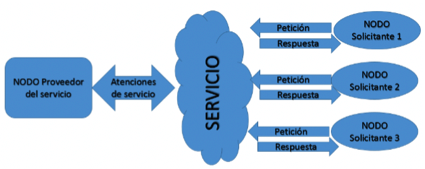
\includegraphics[width=0.8\textwidth]{figures/serviciosros.png}
		\caption{Estructura del sistema de comunicación por Servicios ROS}
		\label{fig.serviciosros}
		\end{center}
\end{figure}

Un elemento que es muy útil para este proyecto es que ROS nos proporciona total compatibilidad con Gazebo mediante un conjunto de paquetes llamados \textit{gazebo\_ros\_pkgs} \footnote{\url{http://wiki.ros.org/gazebo_ros_pkgs}}. En ROS, los paquetes son aquellos donde se incluye todo el código fuente, las librerías usadas y cualquier otro recurso necesario para que funcione el nodo.

La versión de ROS que se utilizará para el desarrollo de este trabajo es ROS Kinetic.

\section{Robot Web Tools}
Comunidad nacida a partir de la de ROS, nos permite conectar aplicaciones web a elementos robóticos gracias a un protocolo llamado Rosbridge. Este protocolo es una especificación de JSON para interactuar con ROS y una capa de transporte para que los clientes se comuniquen mediante WebSockets. Por otro lado, han creado una serie de bibliotecas livianas y fáciles de utilizar de JavaScript que proporcionan una  abstracción de la funcionalidad principal de ROS. Estas bibliotecas son roslibjs, ros2djs y ros3djs, sin embargo en este trabajo solo se utilizará roslibjs.

La biblioteca roslibjs es la encarga de ofrecernos las funcionalidades necesarias para conectarnos, enviar o recibir mensajes ya sea mediante publicación y subscripción, o servicios. La conexión se realiza a un servidor intermedio (servidor Rosbridge), el cual se encarga de gestionar las conexiones, los topic publicados o los servicios activos en cada momento, de modo que cuando te subscribas o realices la petición de un servicio, este servidor se encargue de encaminar la petición mediante WebSockets.

Dado que para este trabajo se va a utilizar JavaScript como lenguaje, se utilizará, en todas las partes relacionadas con ROS, las bibliotecas, servidores y protocolo indicado en esta sección.

\begin{figure}[H]
  \begin{center}
    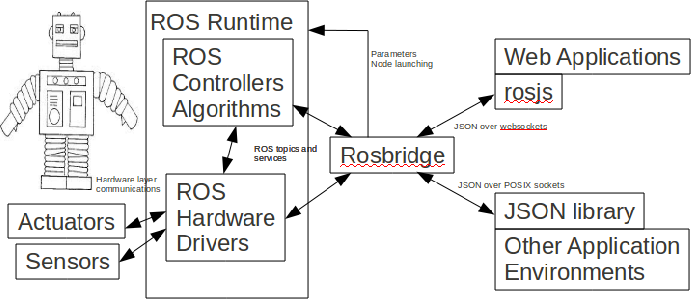
\includegraphics[width=0.8\textwidth]{figures/estructurarosbridge.png}
		\caption{Estructura de una aplicación con Rosbridge}
		\label{fig.estructurarosbridge}
		\end{center}
\end{figure}

\section{Node.js}
Node.js \footnote{\url{https://nodejs.org/es/}} es un entorno multiplataforma del lado del servidor. Concebido con la intención de facilitar la creación de programas de red escalables como puede ser un servidor web, nos permite ejecutar código JavaScript fuera de un navegador y aprovechar las ventajas que nos proporciona su programación orientada a eventos. Su ejecución se lleva a cabo en un único hilo, usando entradas y salidas asíncronas que pueden ejecutarse de manera concurrente, provocando que cada una de ellas necesite de un callback para manejar los eventos. 

Node.js proporciona una serie de módulos básicos que permiten realizar funciones esenciales como puede ser la programación en red asíncrona, el manejo de archivos del sistema, etc. Sin embargo, al ser de código abierto, existe una gran comunidad de desarrolladores que crean nuevos módulos para que cualquiera pueda utilizarlos. Estos módulos son fácilmente compartidos gracias al manejador de paquetes npm \footnote{\url{https://www.npmjs.com/}}, permitiéndonos compilar, instalar y manejar las dependencias de cualquier módulo de terceros que deseemos usar en nuestro proyecto.
 
Por lo general, un proyecto Node.js contendrá al menos dos elementos, un archivo .js que contendrá la lógica del programa escrita en JavaScript y un segundo archivo llamado Package.json que definirá nuestro programa. Este segundo archivo es donde se indican las dependencias que usará nuestro programa y nos facilitará su instalación conjunta usando el comando npm install, así como se referenciará al fichero .js indicado anteriormente.

La versión de Node.js utilizada será la 8.9.1 y la versión del manejador de paquetes npm será la 6.4.0.

\section{WebGL y Three.js}
WebGL \footnote{\url{https://get.webgl.org/}}  es un API multiplataforma utilizada para crear gráficos 3D utilizando tecnologías web, está basado en OpenGL y utiliza parte de su API. WebGL se ejecuta dentro del elemento HTML Canvas, o que proporciona una completa integración con la interfaz DOM. Ofrece ventajas como la compatibilidad con distintos navegadores y plataformas, no es necesario compilar para su ejecución o la interacción con otros elementos del HTML. Sin embargo, debido a que se trata de un API de bajo nivel es complejo de utilizar.

Three.js \footnote{\url{https://threejs.org/}} nace como remedio a la complejidad de usar WebGL. Se trata de una biblioteca desarrollada en JavaScript que permite crear y mostrar gráficos 3D en un navegador web usando una API de alto nivel, proporcionados funciones y objetos para facilitar la creación, interacción y visualización de entornos con gráficos 3D. Utilizando secuencias de código tan simples como \textsl{object = new THREE.Mesh( new THREE.SphereBufferGeometry(75, 20, 10), new THREE.MeshBasicMaterial({color:0xFF0000}))}, nos permite crear una esfera siendo la primera parte donde se define la geometría y la segunda donde se establece el material (puede ser desde un color básico como en este caso, hasta una textura obtenida desde una imagen)

\begin{figure}[H]
  \begin{center}
    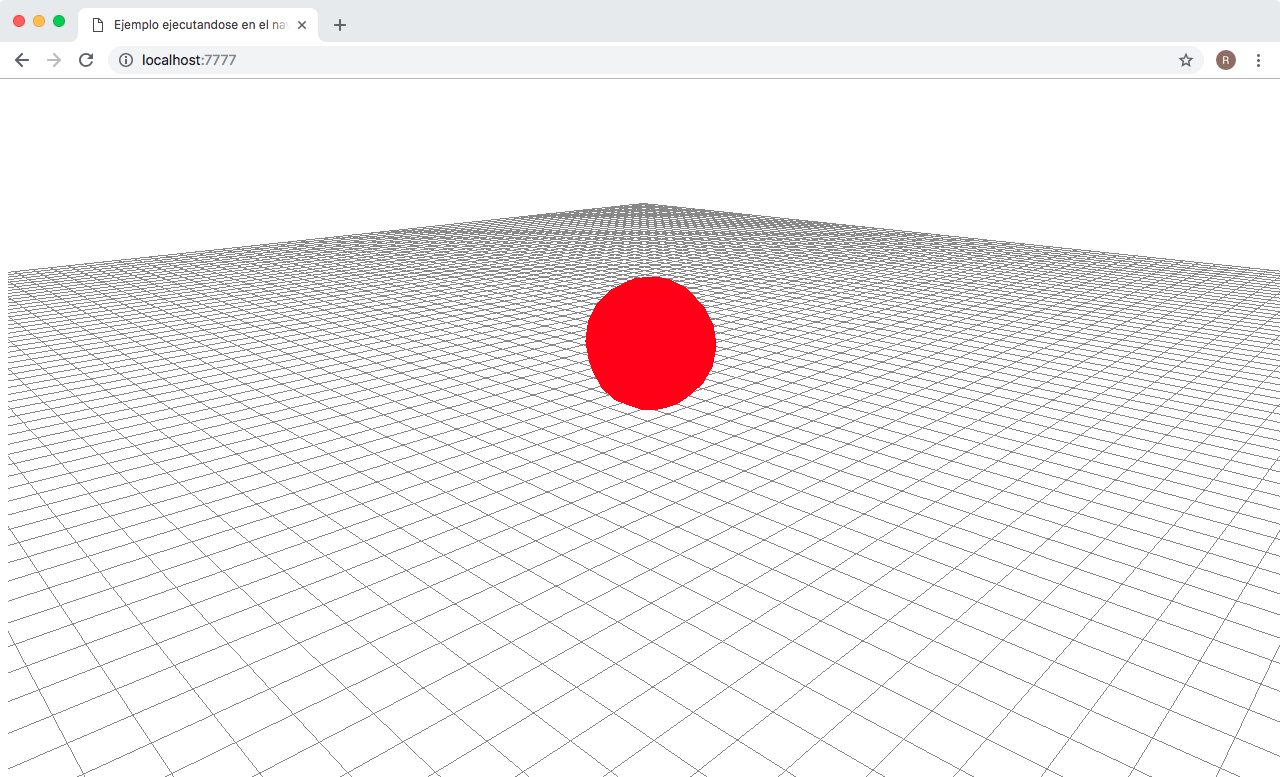
\includegraphics[width=0.8\textwidth]{figures/esferathreejs.png}
		\caption{Esfera creada con la biblioteca Three.js y mostrada en un navegador}
		\label{fig.esferathreejs}
		\end{center}
\end{figure}

\section{WebRTC}
WebRTC \footnote{\url{https://webrtc.org/}}  una tecnología que permite a una aplicación web capturar y transmitir audio y video, así como intercambiar datos con otros navegadores sin necesidad de intermediarios. Este intercambio se realiza de igual a igual (peer-to-peer) sin necesidad de instalaciones o software adicionales. WebRTC proporciona varias API y protocolos interrelacionados para dar a los navegadores y aplicaciones móviles la capacidad de intercambiar elementos multimedia en tiempo real (Real Time Communications). Esta tecnología esta soportada en los principales navegadores y tiene el soporte de Google.

En este proyecto, usaremos WebRTC para la adquisición de del video obtenido a través de una cámara web. Para lograr este objetivo, se utilizará el API de WebRTC Media Stream, que nos proporcionará la descripción de los flujos de datos de audio y video, los métodos para trabajar con ellos, la conexión con los dispositivos para adquirirlos, las limitaciones asociadas a cada tipo de datos o los eventos asociados al proceso.

\section{El framework Electron}
Electron \footnote{\url{https://electronjs.org/docs}}  es un framework de código abierto desarrollado por GitHub. Comenzó su desarrollo en 2013, en el mismo grupo de trabajo del editor Atom \footnote{\url{https://atom.io/}}. Concebido con la ides de permitir la creación de aplicaciones de escritorio multiplataforma con tecnologías web. Electron es la combinación de NodeJS y Chromium \footnote{\url{https://www.chromium.org/Home}} en una misma ejecución.

La arquitectura de una aplicación que utiliza Electron esta formada por dos procesos: Principal y Renderizador. 

El proceso principal es el encargado de generar la interfaz de usuario mediante la creación de páginas web y las administra de modo que es posible mostrar más de una página web al mismo tiempo. Esta labor se realiza mediante la instancia al objeto BrowserWindow de Electron, ejecutándose una página web cada vez que se instancia. Cuando se destruye una de estas instancias, se está cerrando esa página web. Cada aplicación con Electron debe constar de un único proceso principal, y corresponderá al script main del archivo package.json.

El proceso renderizador es cada instanacia al objeto BrowserWindow y la ejecucuion de la página web correspondiente. Una aplicación con Electron puede tener multitud de procesos renderizadores, siendo cada uno independiente del resto. Cada proceso solos se preocupa de la página web que se esta ejecutando en él.

Electron es totalmente compatible con NodeJS tanto en el proceso principal como en el renderizador, por lo que todas las herramientas disponibles para Node.js, también lo están para Electron. Así mismo, es posible utilizar módulos Node.js alojados en el repositorio de paquetes npm mencionado anteriormente. Este nos aporta un gran número de ventajas como una mayor seguridad al cargar contenido remoto, tener siempre actualizadas las aplicaciones o tener un gran número de bibliotecas disponibles.

Todas las aplicaciones que se desarrollarán en este trabajo podrán ser ejecutadas utilizando Electron, lo que nos permite utilizarlas en cualquier plataforma o, incluso, empaquetarlas usando npm o mediante un archivo Asar \footnote{\url{https://github.com/electron/asar}}.

\subsection{Adaptar una aplicación web para ser usada con Electron}

Una aplicación que utiliza Electron estará formada por un archivo HTML, un fichero main.js que definirá la ventana donde se mostrará el fichero HTML y se creará la misma, y, al igual que se indica en la sección de Node.js, el archivo package.json que definirá la aplicación en Electron (nombre, versión, descripción, etc.), se indicaran las dependencias a módulos externos y el fichero main.js para que creé la aplicación. Una vez que contamos con al menos estos tres elementos, podemos instalar las dependencias mediante npm install (igual que para Node.js) y ejecutar la aplicación mediante npm start o npm test (dependerá de como hayamos definido package.json).

\subsubsection{package.json}
El cometido de este archivo definirá las dependencias de paquetes de terceros que tendrá la aplicación web, definir las características de la aplicación (nombre, versión, autor, etc.) y, lo que es más importante, de que manera se lanzara la aplicación y el archivo que se debe ejecutar al lanzarla. A continuación se muestra lo que podría ser un ejemplo de un package.json:
\begin{lstlisting}[frame=single]
{
  "name": "Ejemplo",
  "version": "0.1.0",
  "main": "main.js",
  "scripts": {
    "start": "electron ."
  },
  "dependencies": {
      "electron": "^1.8.4",
  }
}
\end{lstlisting}

Como se puede apreciar, la versión de Electron que se utilizará será la 1.8.4.

\subsubsection{main.js}
El archivo "main.js" indicado anteriormente, contendrá muy pocas líneas de código al tratarse de un elemento totalmente externo a la aplicación y no tener ningún papel en su funcionamiento, únicamente es necesario para ejecutar la aplicación utilizando Electron. A continuación se muestra el código de este archivo:

\begin{lstlisting}[frame=single]
const app = require('electron')
const path = require('path')
const url = require('url')

let win;

function createWindow () {
  win = new BrowserWindow({width: 1800, height: 1000})
  win.loadURL(url.format({
    pathname: path.join(__dirname, 'camserver.html'),
    protocol: 'file:',
  }))
  
app.on('ready', createWindow)

\end{lstlisting}

Lo primero que se realiza es definir los módulos que se requieren para que funcione correctamente y que se utilizaran en el resto del código. Posteriormente, se define el tamaño de la ventana, en este caso la ventana será de 1800 pixeles de ancho y 1000 de alto. Mediante win.loadURL se simula el funcionamiento de un navegador y como gestionan las diferentes URLs, este método se le pasará como parámetros el archivo HTML principal de la aplicación web, el protocolo que este caso es "file:", al estar queriendo mostrar directamente de un archivo HTML (si quisiéramos mostrar mediante Electron el contenido de una página web ya existente, protocol tomaría el valor "http:"). Finalmente, la última línea de código llamará a la función que crea la ventana y muestra el HTML en el momento que Electron haya terminado de inicializarse y está preparado para la creación de la ventana.


En la figura 3.6 se muestra el mismo HTML ejecutado con Node.js y con Electron. Como se puede apreciar, el resultado es el mismo.

\begin{figure}[H]
  \begin{center}
    \subfigure[Node.js]{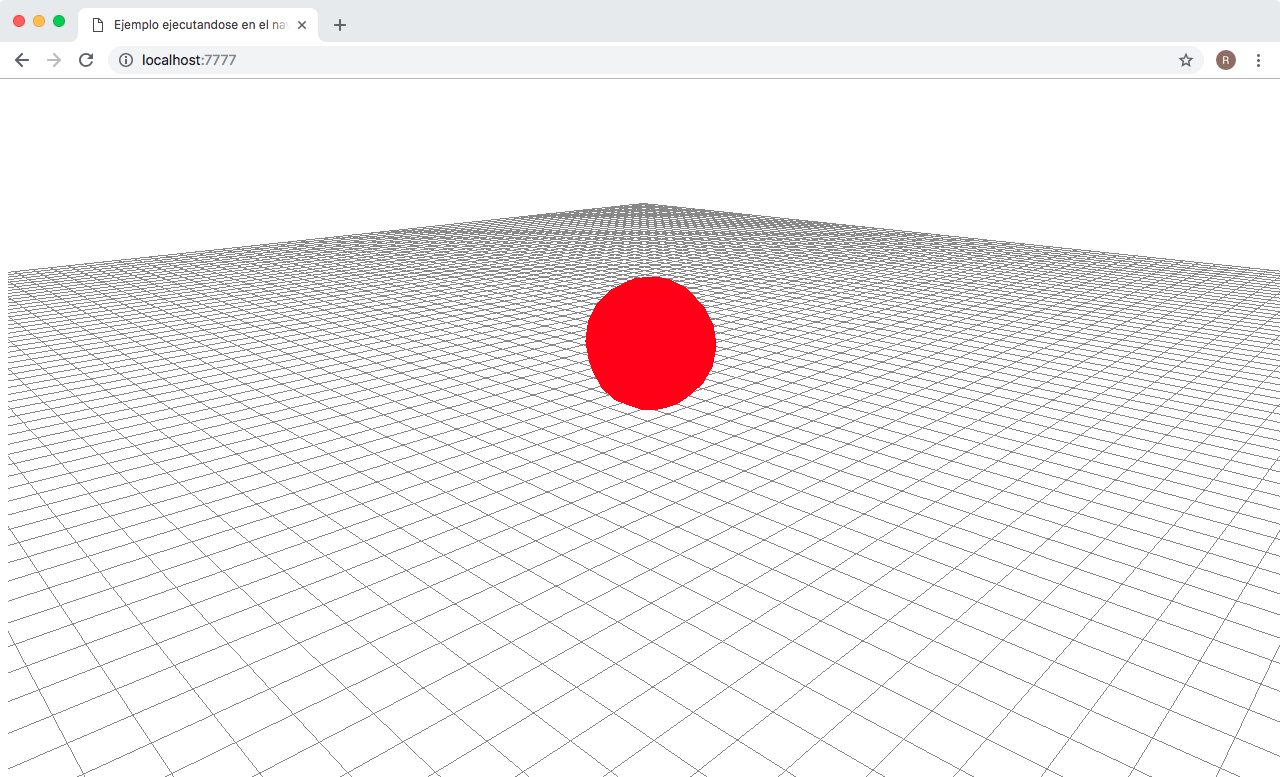
\includegraphics[width=0.4\textwidth]{figures/esferathreejs.png}}
    \subfigure[Electron]{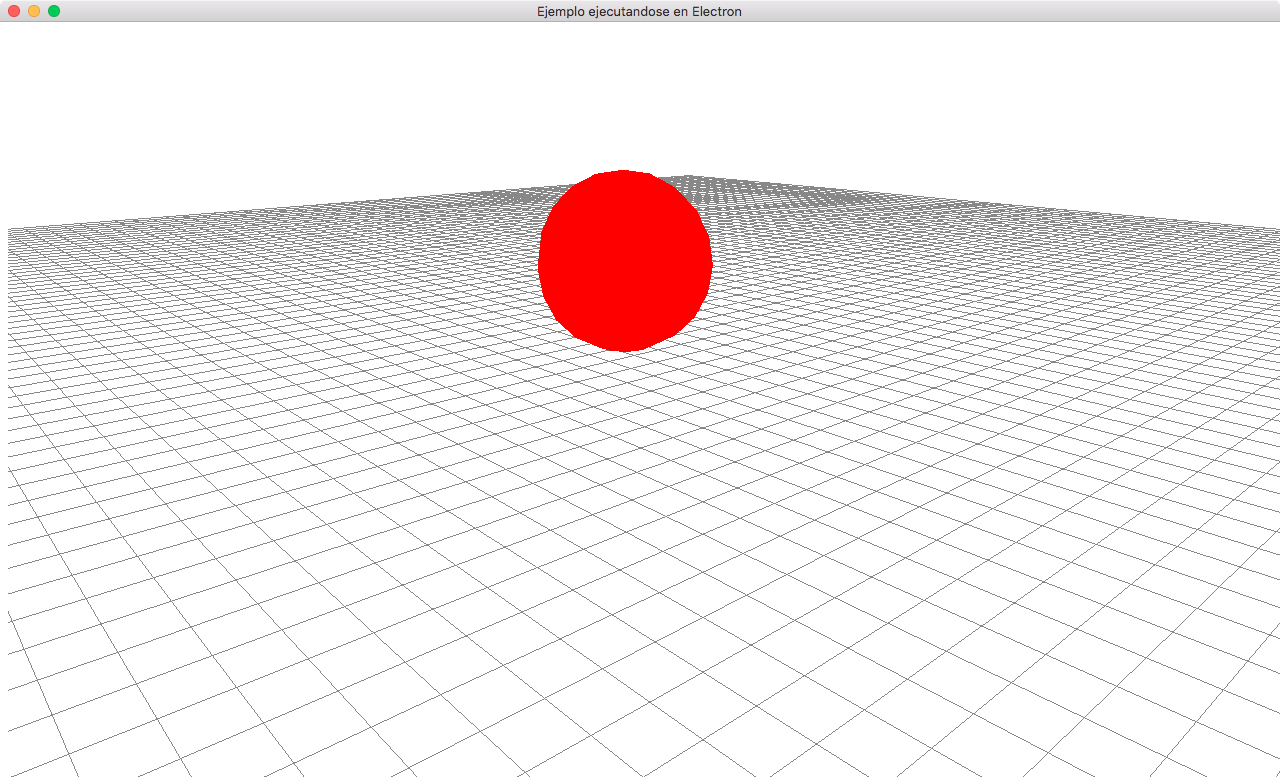
\includegraphics[width=0.4\textwidth]{figures/ejemploelectron.png}}
    \caption{Ejemplo de la esfera anterior ejecutado con Node.js y con Electron}
     \label{fig.ejemplohtmlcomm}
     \end{center}
\end{figure}







\lhead[]{CAP\'ITULO \thechapter. VISORES}
\chapter{Visores web modificados}\label{cap.Visores}

\lhead[]{CAP\'ITULO \thechapter. VISOR3D}
\chapter{Visor web dinámico de objetos 3D}\label{cap.visor3d}
En este capítulo se va a tratar la creación de un nuevo visor de primitivas 3D (objetos, puntos y segmentos) con tecnologías web. Este visor, al que se ha nombrado como 3DVizWeb,  abrirá la posibilidad de obtener datos por una cámara o sensor y mostrar una representación 3D de los mismos.
\section{Diseño}
Este visor está elaborado usando JavaScript y HTML como lenguajes de programación, y se usará el middleware ICE para la interconexión con los clientes que enviarán los datos a mostrar. En la figura 5.1 se muestra el diagrama de bloques:

\begin{figure}[H]
  \begin{center}
    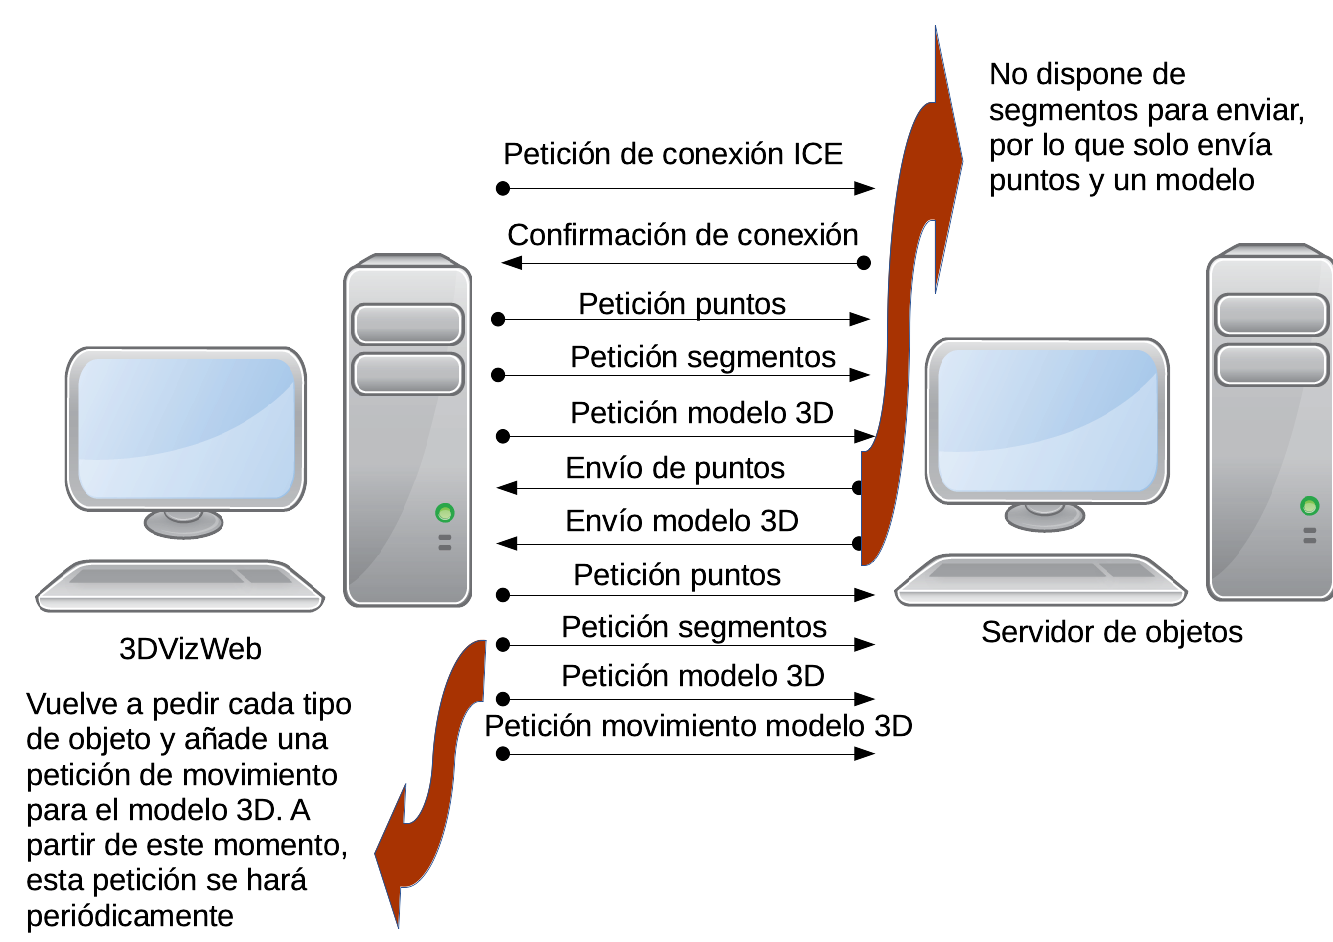
\includegraphics[width=0.8\textwidth]{figures/esquemavisor.png}
		\caption{Diagrama de bloques del sistema}
		\label{fig.diseno3dviz}
		\end{center}
\end{figure}

En la figura 5.2 se muestra el diseño del visor de una manera mas detallada:

\begin{figure}[H]
  \begin{center}
    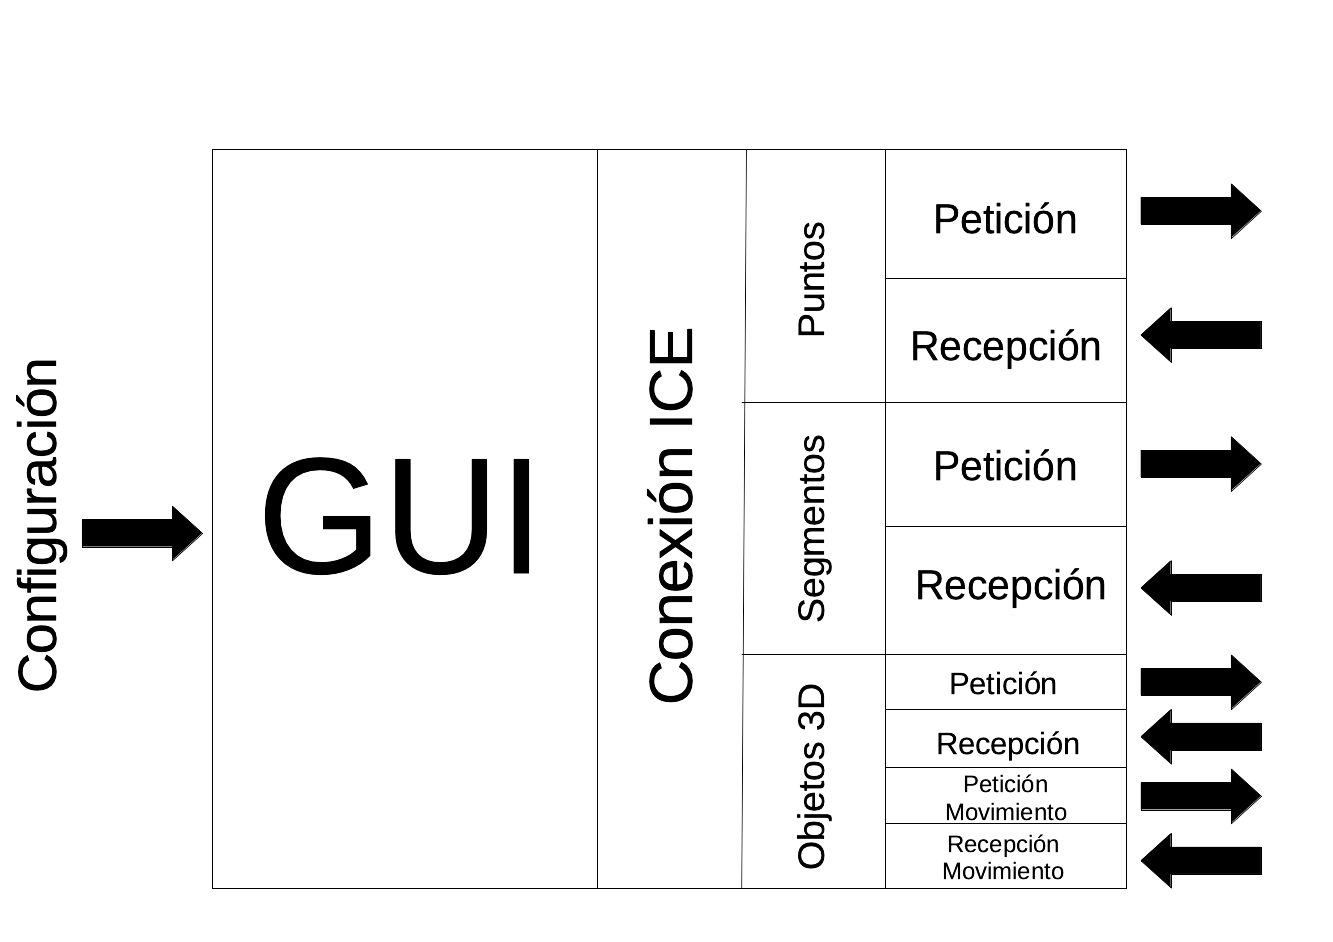
\includegraphics[width=0.8\textwidth]{figures/diseno3dviz.png}
		\caption{Diseño del visor 3D}
		\label{fig.diseno3dviz}
		\end{center}
\end{figure}
La herramienta está dividida en dos partes: la interfaz gráfica y las conexiones ICE.

La parte correspondiente a la interfaz gráfica es la que da origen al visor y marca como se definen cada uno de los tipos de objetos que es capaz de mostrar. Hay tres tipos de primitivas 3D que el visor es capaz de visualizar: puntos segmentos y objetos.

Las conexiones ICE con el servidor incluyen varias partes claramente segmentadas. Estas partes corresponden a la petición y recepción de cada tipo de primitiva al servidor, haciendo especial hincapié en los objetos 3D que contarán con las peticiones y recepciones para mostrar nuevos objetos. El formato del archivo que admite el visor puede ser del tipo ``dae'' o ``obj''. Estos dos formatos son los más utilizados a la hora de crear objetos 3D y por tanto se considera que dando soporte a los dos formatos permite usar cualquier objeto que se desee. Los objetos se podrán mover en 3D y el visor ofrece mecanismos eficientes para que las aplicaciones, mediante  peticiones y recepciones, puedan mover los objetos existentes en la escena que se está visualizando.

\section{Configuración}
Dado que el visor en su interfaz gráfica únicamente muestra la escena donde se visualizan los objetos, es necesario utilizar una alternativa para configurar los datos de conexión (ip y puerto de escucha) y otros parámetros configurables (posición inicial de la cámara, tamaño de los puntos, tamaño de los segmentos y periodo de tiempo entre peticiones de cada tipo de objeto) antes de arrancar el visor. Para realizar está configuración se vuelve a utilizar un archivo en formato ``YAML'', como se explica en la sección 4.1.6 de este trabajo.

Los parámetros que se pueden configurar para el visor son los siguientes:
\begin{itemize}
\item Dirección IP. Por defecto es ``localhost''
\item Puerto. Por defecto es ``11000''
\item Tiempo de refresco para la petición de puntos en milisegundos. Por defecto son 1000 ms
\item Tiempo de refresco para la petición de segmentos en milisegundos. Por defecto son 1000 ms
\item Tiempo de refresco para la petición de objetos 3D en milisegundos. Por defecto es 1 ms
\item Tiempo de refresco para la petición del movimiento de objetos en milisegundos. Por defecto son 1000 ms
\item Grosor de los segmentos en pixeles. Por defecto son 2 pixeles.
\item Tamaño de los puntos en pixeles. Por defecto son 8 pixeles.
\item Posición inicial de la cámara desde que se observa la escena. Está formada por las coordenadas ``x'', ``y'' y ``z'' , siendo por defecto ``50'', ``20'' y ``100'' respectivamente.
\end{itemize}

\section{Interfaz gráfica}
La interfaz gráfica del visor está diseñada usando WebGL, y más concretamente usando la biblioteca Three.js descrita en capítulos anteriores. La interfaz gráfica de la aplicación, la ventana, la ocupa íntegramente el visor 3D, no tendrá ningún elemento adicional como pueden ser botones o diales. La escena 3D muestra inicialmente una rejilla que hará de plano horizontal, cuyo centro será la posición (0, 0, 0) del eje de coordenadas. Además ha sido necesario añadir iluminación y una cámara para poder visualizar la escena desde ella.

\subsection{Escena base}
El visor está contenido dentro de un elemento HTML \texttt{<canvas>}. En este elemento se crea una nueva escena usando la función de Three.js \texttt{THREE.Scene()} y se renderiza usando \texttt{THREE.WebGLRenderer()}. Posteriormente se crea una cámara con perspectiva utilizando \texttt{THREE.PerspectiveCamera()} ubicándola en una posición predeterminada (la indica en el archivo de configuración anteriormente indicado) y podrá ser controlada mediante teclado o ratón. Finalmente, para visualizar correctamente la escena se añaden varias luces puntuales a lo largo de la misma, así como una iluminación de ambiente utilizando \texttt{THREE.PointLight()} y \texttt{THREE.AmbientLight()} pasándole como parámetros el color de la luz y la intensidad de la misma.

Una vez tenemos una escena completamente visible, se procede a crear y añadir la rejilla. La función existente en la biblioteca Three.js, \texttt{new THREE.GridHelper()}, permite definirla muy fácilmente introduciendo por parámetro a la función la separación, cantidad y color de las líneas de división que generan la rejilla. Para añadirla a la escena, basta con usar \texttt{.add(rejilla)}. Estos elementos forman la escena base del visor.

\begin{figure}[H]
  \begin{center}
    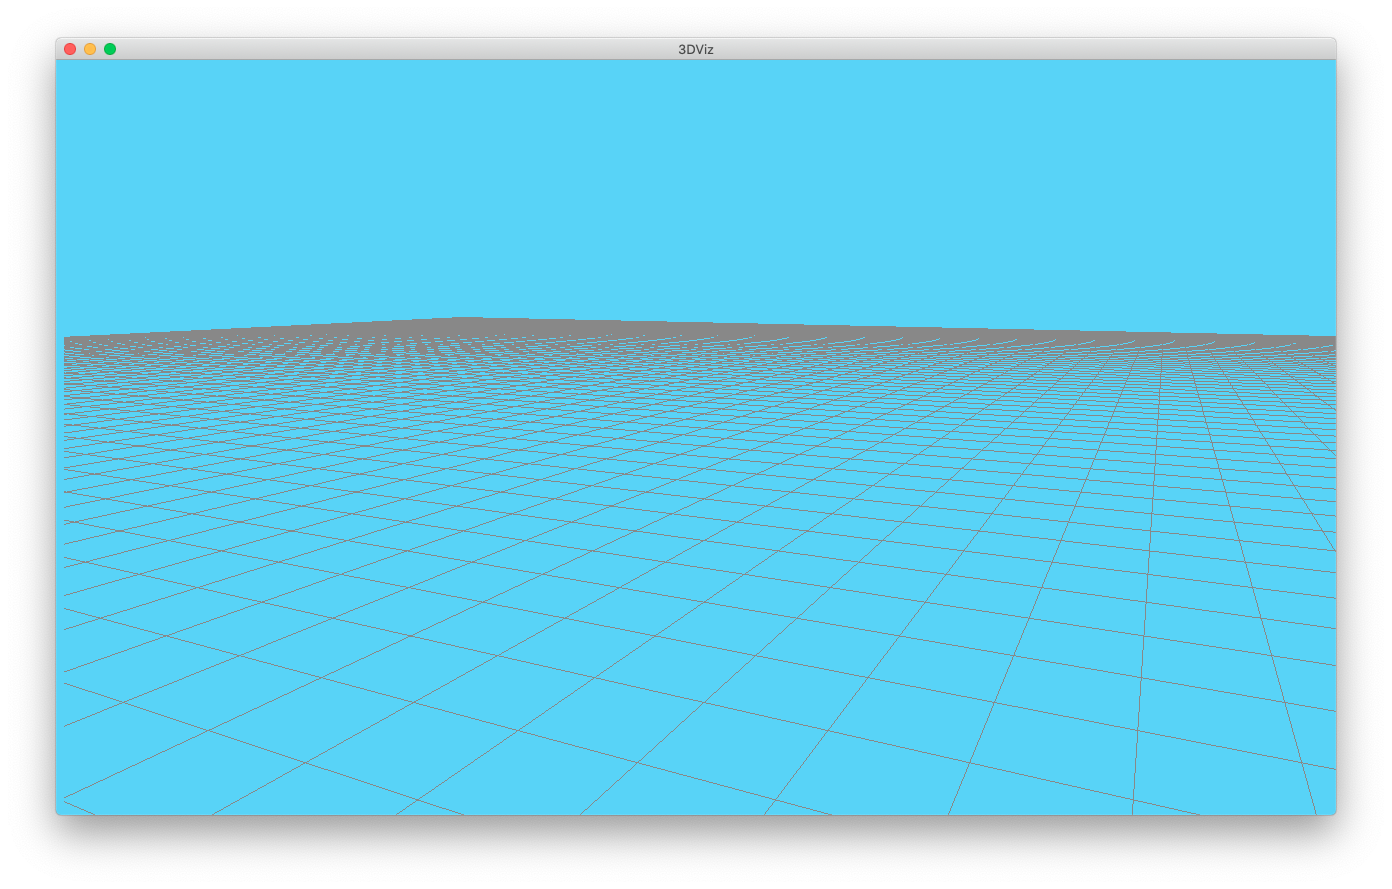
\includegraphics[width=0.8\textwidth]{figures/interfazinicial.png}
		\caption{Interfaz gráfica con la escena base del visor}
		\label{fig.interfazinicial}
		\end{center}
\end{figure}

\subsection{Visualización de puntos}
Un punto es el elemento geométrico más simple que es posible representar. Sin embargo, pese a ello, proporciona al visor la capacidad de realizar representaciones más complejas mediante el uso de una gran cantidad de puntos. Para representar puntos, únicamente es necesarios una posición en el eje de coordenadas, el tamaño del punto y el material o color que se quiera darle. 
La biblioteca Three.js proporciona una serie de elementos para facilitar la creación de puntos. El código se muestra en el cuadro 5.2.
\begin{lstlisting}[caption= Creación y visualización de puntos, label=cod.crearpunto]
function addPoint (point){
	var geometry = new THREE.Geometry();
	geometry.vertices.push( new THREE.Vector3(point.x,point.z,point.y));
	var material = new THREE.PointsMaterial( { size: 8, sizeAttenuation: false, 
										alphaTest: 0.5, transparent: true } );
	material.color.setRGB( point.r, point.g, point.b);
	var particles = new THREE.Points( geometry, material );
	particles.name ="points";
	scene.add( particles );}
\end{lstlisting}
Primero es necesario indicar que se está creando una figura geométrica para posteriormente definirla. Al tratarse de un punto, solo va a tener un vértice por lo que al definir la geometría se indica que serán vertices pero únicamente se proporciona uno de ellos mediante un vector ``x'', ``y'' y  ``z'', que serán las coordenadas centrales del punto a representar. Cabe destacar que dado que el sistema de coordenadas de obtención de los datos no se corresponde con el sistema de coordenadas gráficas de la escena, hay que realizar una conversión. Si recibimos un punto con coordenadas (x,y,z), en la escena corresponderán a (x,z,y). 


Una vez definida la geometría, lo siguiente es definir el tamaño del punto, su aspecto y, posteriormente, su color. El tamaño indicado en el código es de 8 píxeles, sin embargo este tamaño es configurable a través de un fichero de configuración indicado en la sección anterior. El color del punto se definirá mediante sus componentes RGB, que vienen indicadas por el servidor que transmite el punto. Las componentes vendrán separadas en ``R'', ``G'' y ``B'', y su valor oscilará entre ``0'' y ``1'' (se corresponde con el valor ``255'') para cada una de ellas.

Finalmente creamos el punto a partir de la geometría y el material proporcionado, le atribuimos el nombre ``punto'' para poder borrarlo discrecionalmente, si así se desea, y se añade a la escena.
Esta función será invocada cada vez que se reciba uno o más puntos procedentes del servidor. La figura 5.4 muestra varios puntos en el visor.
\begin{figure}[H]
  \begin{center}
    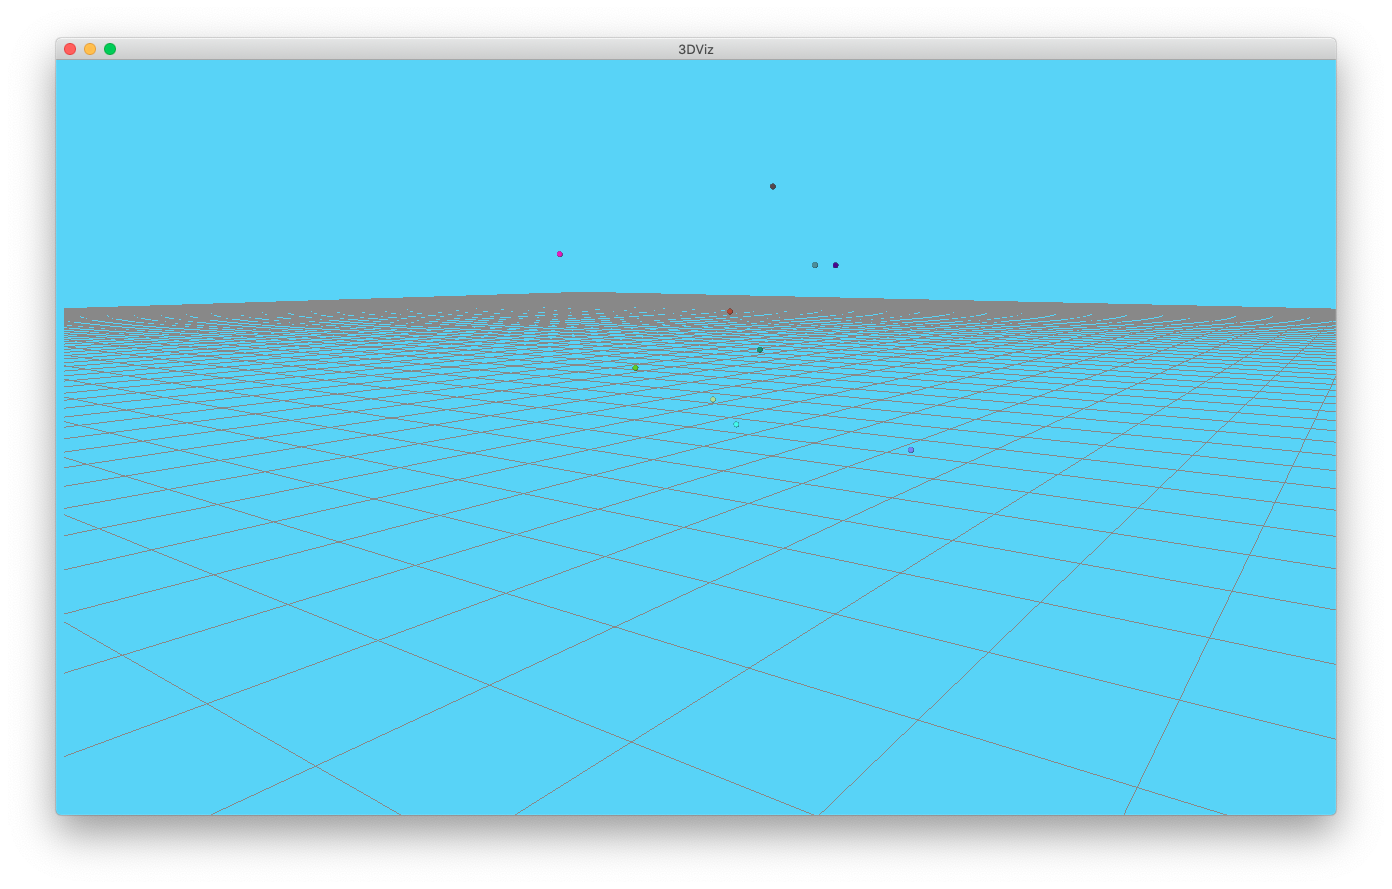
\includegraphics[width=0.8\textwidth]{figures/visualizarpuntos.png}
		\caption{Varios puntos de distintos colores visualizados en el visor}
		\label{fig.visualizarpuntos}
		\end{center}
\end{figure}
\subsection{Visualización de segmentos}
El segmento es otro de los elementos fundamentales de la geometría y se puede definir cómo un fragmento de recta que está comprendido entre dos puntos. Teniendo en cuenta esto, para  representarlo únicamente es necesario las coordenadas de dos puntos, el grosor del segmento y el color del mismo. En el cuadro 5.3 se muestra el código para la creación de un segmento.
\begin{lstlisting}[caption= Creación y visualización de segmentos, label=cod.crearsegmento]
function addLine(segment){
	var geometry = new THREE.Geometry();
	geometry.vertices.push(
		new THREE.Vector3(segment.fromPoint.x, segment.fromPoint.z, 
							segment.fromPoint.y),
		new THREE.Vector3(segment.toPoint.x, segment.toPoint.z, 
							segment.toPoint.y));
	var material = new THREE.LineBasicMaterial();
	material.color.setRGB(segment.r, segment.g, segment.b);
	material.linewidth = 2;
	line = new THREE.Line(geometry,material);
	line.name = "line";
	scene.add(line);}
\end{lstlisting}
La estructura es muy similar que la función para crear un punto. Al igual que para allí, se necesita definir la geometría pero en este caso vamos a tener dos vértices en lugar de uno (dos puntos). El primer vértice será desde el lugar donde comience el segmentos, y el segundo vértice el lugar donde termine. En otras palabras, el segmento será la unión entre el primer vértice con el segundo. Las coordenadas de estos dos puntos serán proporcionadas por el servidor. Al igual que en el caso del punto, el sistema de coordenadas del servidor no coincide con el sistema del visor, por lo que se debe realizar la misma conversión, es decir la coordenada ``z'' que envíe el servidor, se corresponde a la coordenada ``y'' del visor, y viceversa.

Posteriormente, se definen el material y aspecto del segmento proporcionando el grosor y el color. En el código anterior, el grosor es de 2 píxeles, sin embargo este parámetro es configurable mediante el fichero de configuración explicado anteriormente. El color, por el contrario, vendrá definido por el servidor mediante sus componentes RGB, que al igual que para el caso del punto, vendrán segmentadas en ``R'', ``G'' y ``B'', valiendo entre ``0''  y ``1'' (corresponde al valor ``255'').

Finalmente se crea el segmento a partir de la geometría y el material proporcionado, dándole el nombre ``line'' para borrar selectivamente solo los segmentos. Una vez generado el elemento, se añade a la escena. Esta función será la invocada cada vez que se reciba uno o más segmentos desde el servidor. La figura 5.5 muestra varios segmentos en el visor.
\begin{figure}[H]
  \begin{center}
    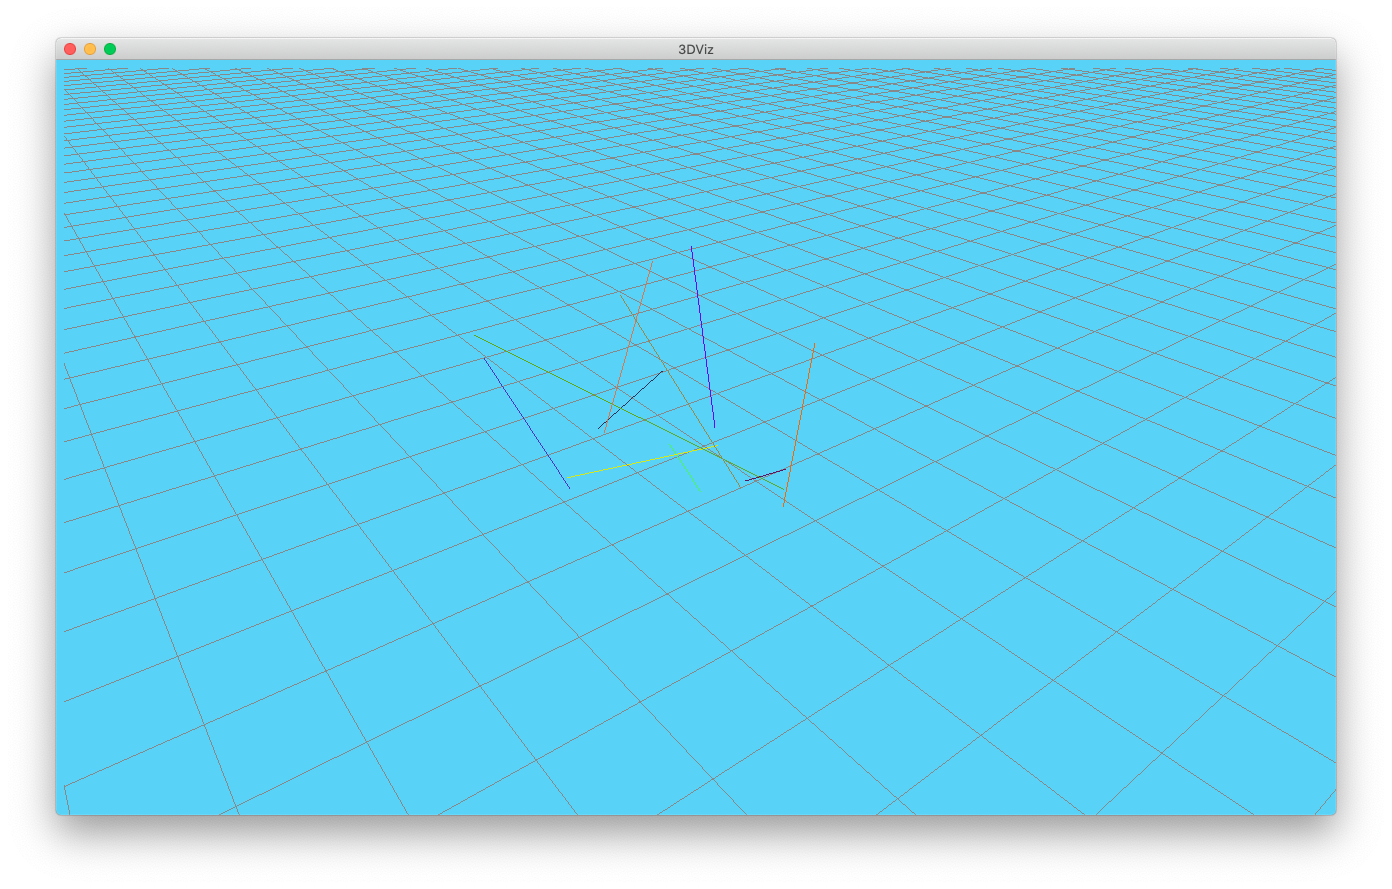
\includegraphics[width=0.8\textwidth]{figures/visualizarlineas.png}
		\caption{Varios segmentos de distintos colores visualizados en el visor}
		\label{fig.visualizarsegmentos}
		\end{center}
\end{figure}

\subsection{Visualización de objetos 3D}
Un objeto 3D es una representación matemática de un objeto tridimensional que se puede guardar en un archivo de definición de geometría. El visor es capaz de representar dos formatos diferentes de estos archivos, ``obj'' y ``dae'', y moverlos cuando el servidor lo requiera. 

\subsubsection{Creación y visualización de los objetos 3D}
Los objetos 3D pueden ser recibidos o bien a través del archivo completo como texto plano, o bien a través de una URL. El visor será capaz de representar el objeto 3D y ubicarlo en la posición indicada. El código del cuadro 5.4 muestra como identificar si el objeto viene como texto plano o URL, para posteriormente invocar a la función correspondiente dependiendo el formato del objeto.
\begin{lstlisting}[caption= Creación y visualización de objetos 3D, label=cod.crearobjetos3d]
function addObj(obj,pos){
	var type = obj.obj.split(":");
	if (type[0] == "https" || type[0] == "http") {
		var url = obj.obj
	} else{
		var file = new Blob([obj.obj], {type:'text/plain'});
		var url  = window.URL.createObjectURL(file);
	}
	if (obj.format == "obj"){
		loadObj(url, obj,pos)
	} else if (obj.format == "dae") {
		loadDae(url,obj.pos);
	}
}
\end{lstlisting}
Cuando se recibe el objeto procedente del servidor, lo primero que se hace es trocear el mensaje para poder analizarlo y esclarecer si lo que está enviando el servidor es el archivo completo o una URL al archivo completo. De tratarse de una URL, debe contener ``https://'' o ``http://'', se puede trocear mediante ``:'' y, con una sentencia condicional verificar si la primera parte de la separación es ``https'', ``http'' u otra cosa. En caso de ser ``https'' o ``http'', lo que lo que se ha recibido es la ruta al archivo, sino el objeto completo y se debe generar un archivo virtual utilizando el objeto \textit{Blob} (objeto que representa un fichero) y posteriormente generar una URL virtual, ya que se ha recibido como texto plano y para poder visualizarlo es necesario que el objeto sea un archivo y se tenga una ruta, una URL local, al mismo. Como se puede ver, por ambos caminos tenemos una URL, de modo que ya es posible representar el objeto.

Una vez se tiene la URL del objeto, es necesario saber el formato del archivo del objeto (``obj'' o ``dae''), ya que no se carga el objeto de la misma forma. Identificar el formato es sencillo, ya que vendrá indicado por el servidor y, dependiendo del formato, se invoca a la función de procesamiento correspondiente pasando por parámetro la URL y la posición deseada del objeto en el visor (coordenadas y orientación del objeto) recibidas del servidor.

\begin{itemize}
\item {\textbf{\underline{Representación de objetos del tipo obj}}

Un archivo con formato ``obj'' es conocido como Wavefront 3D Object File y el formato fue desarrollado por Wavefront Technologies. Es usado para un objeto tridimensional que contiene las coordenadas 3D (líneas poligonales y puntos), mapas de textura, y otra información de objetos. La biblioteca Three.js proporciona un API para poder cargar y mostrar un objeto de este tipo a través de una URL. 

El código del cuadro 5.5 carga y muestra un objeto ``obj'':

\begin{lstlisting}[caption= Carga y visualización de objetos ``obj'', label=cod.objetosobj]
function loadObj(url,obj,pose3d){
	var loader = new THREE.OBJLoader();
	loader.load(
		url,
		function(object){
			object.name = obj.id;
			id_list.push(obj.id);
			object.position.set(pose3d.x, pose3d.z, pose3d.y);
			object.rotation.set(pose3d.rx*toDegrees, pose3d.rz * toDegrees, 
							pose3d.ry * toDegrees);
			scene.add(object);
		},
		function (xhr){
		},
		function (error){
			console.log(error);
		});
}
\end{lstlisting}

Lo primero que hace es inicializar el API de Three.js para cargar un objeto ``obj'' y llama a la función del API encargada de cargar el objeto. Esta función tiene como parámetros la URL y otras tres funciones más. La primera es la encargada de cargar el objeto y mostrar el mismo en el visor, la segunda se ejecuta mientras se está cargando el objeto (por ejemplo, para mostrar una barra de progreso) y la última se ejecutará si ocurre algún error durante la carga. La primera función es la importante, en ella identificamos al objeto dándole un \texttt{id} previamente establecido y lo añadimos a un array, y que se explicará en siguientes secciones, para poder borrarlo o moverlo posteriormente. También posiciona el objeto en 3D mediante las coordenadas enviadas por el servidor, teniendo en cuenta el problema explicado en las secciones anteriores acerca de la disparidad entre los sistemas de coordenadas. Igualmente orienta el objeto 3D mediante la rotación correspondiente a cada eje, que es enviada en radianes y se debe convertir a grados.
Finalmente, se añade el objeto al visor.}

\item{\textbf{\underline{Representación de objetos del tipo dae}}

El formato ``dae'' de ficheros, también conocido como ``Collada'', es un formato de archivos 3D utilizado para el intercambio activo entre programas de gráficos y basado en el esquema XML Collada. La biblioteca Three.js proporciona un API para la carga y visualización de este formato a partir de una URL. El código del cuadro 5.6 carga y muestra un objeto ``dae'':
\begin{lstlisting}[caption= Carga y visualización de objetos ``dae'', label=cod.objetosdae]
function loadDae (url,obj,pose3d){
	var loader = new THREE.ColladaLoader();
	loader.load(url, 
		function (object) {
			object = object.scene;
			object.name = obj.id;
			id_list.push(obj.id);
			object.position.set(pose3d.x, pose3d.z, pose3d.y);
			object.rotation.set(pose3d.rx*toDegrees, pose3d.rz * toDegrees, 
							pose3d.ry * toDegrees);
			scene.add( object );		
		},
		function (xhr){
		},
		function (error){
			console.log(error);
		});
}
\end{lstlisting}
Como se puede apreciar, el código es igual que el utilizado para el formato ``obj'', únicamente cambia la inicialización del API que en este caso es el API para cargar un archivo ``dae'' y la obtención del objeto, ya que se debe referenciar al mismo para poder cargarlo en el visor. El resto del código es el mismo para ambos casos.}
\end{itemize}
Estas funciones de carga serán invocadas cada vez que se reciba un objeto nuevo que mostrar. Si bien en esta memoria se muestra dos funciones diferentes para cargar un objeto ``obj'' o ``dae'' por claridad, en el código final se agrupan en una única función, utilizando en ella la sentencia condicional para identificar el tipo de formato del objeto, evitándonos el uso de código repetido. La figura 5.6 muestra dos objetos (cada uno de un formato) en el visor.

\begin{figure}[H]
  \begin{center}
    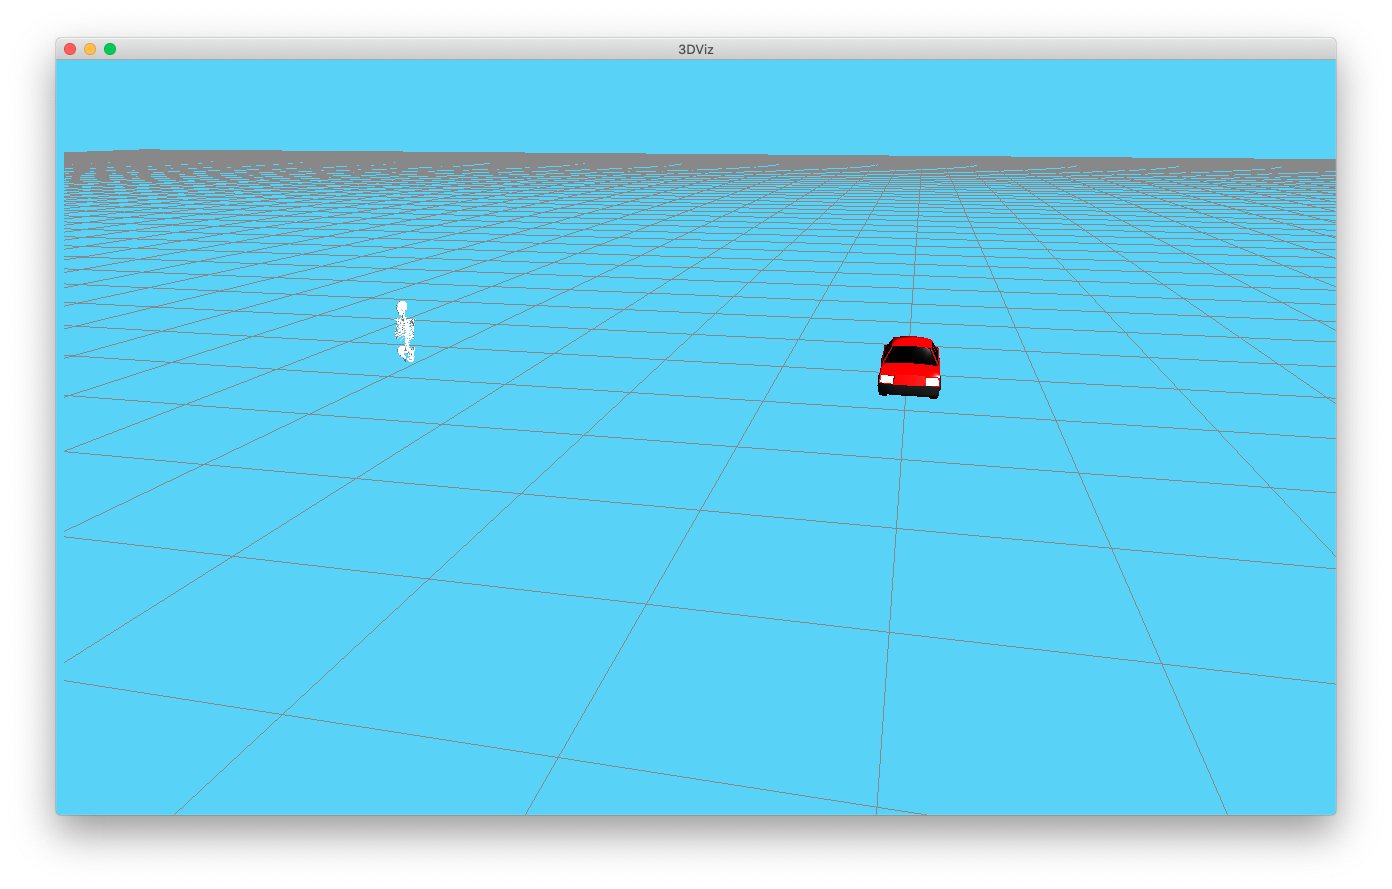
\includegraphics[width=0.8\textwidth]{figures/visualizarmodel.png}
		\caption{Objetos 3D mostrados en el visor}
		\label{fig.visualizarmodel}
		\end{center}
\end{figure}
\subsubsection{Movimiento de los objetos 3D}
A diferencia de un punto o un segmento, que es más sencillo eliminarlo y volver a crearlo en la nueva posición, un objeto 3D interesa reubicarlo a la nueva posición en lugar de eliminarlo y crearlo de nuevo, lo que conllevaría tener que enviar una URL o un texto plano con el archivo del objeto y cargarlo de nuevo, teniendo un retardo y carga de trabajo importante para el visor.

Al haber identificado el objeto mediante un \texttt{id} único (en el caso del punto y la recta, el \texttt{id} es el mismo para cada elemento), permite realizar el movimiento.
\begin{lstlisting}[caption= Código para realizar el movimiento de los objetos 3D, label=cod.moverobjetos]
function moveObj(objeto){
	selectedObject = scene.getObjectByName(objeto.id);
	selectedObject.position.set(objeto.x, objeto.z, objeto.y);
	selectedObject.rotation.set(objeto.rx*toDegrees, objeto.rz * toDegrees, 
							objeto.ry * toDegrees,);
}
\end{lstlisting}
Como se puede apreciar, mover el objeto es mucho más rápido y sencillo que eliminarlo y crearlo de nuevo. Primero se selecciona el objeto mediante el identificador, posteriormente se reubica el objeto seleccionado a las nuevas coordenadas y se aplica la nueva orientación. La figura 5.7 corresponde a los objetos anteriores desplazados y rotados:
\begin{figure}[H]
  \begin{center}
    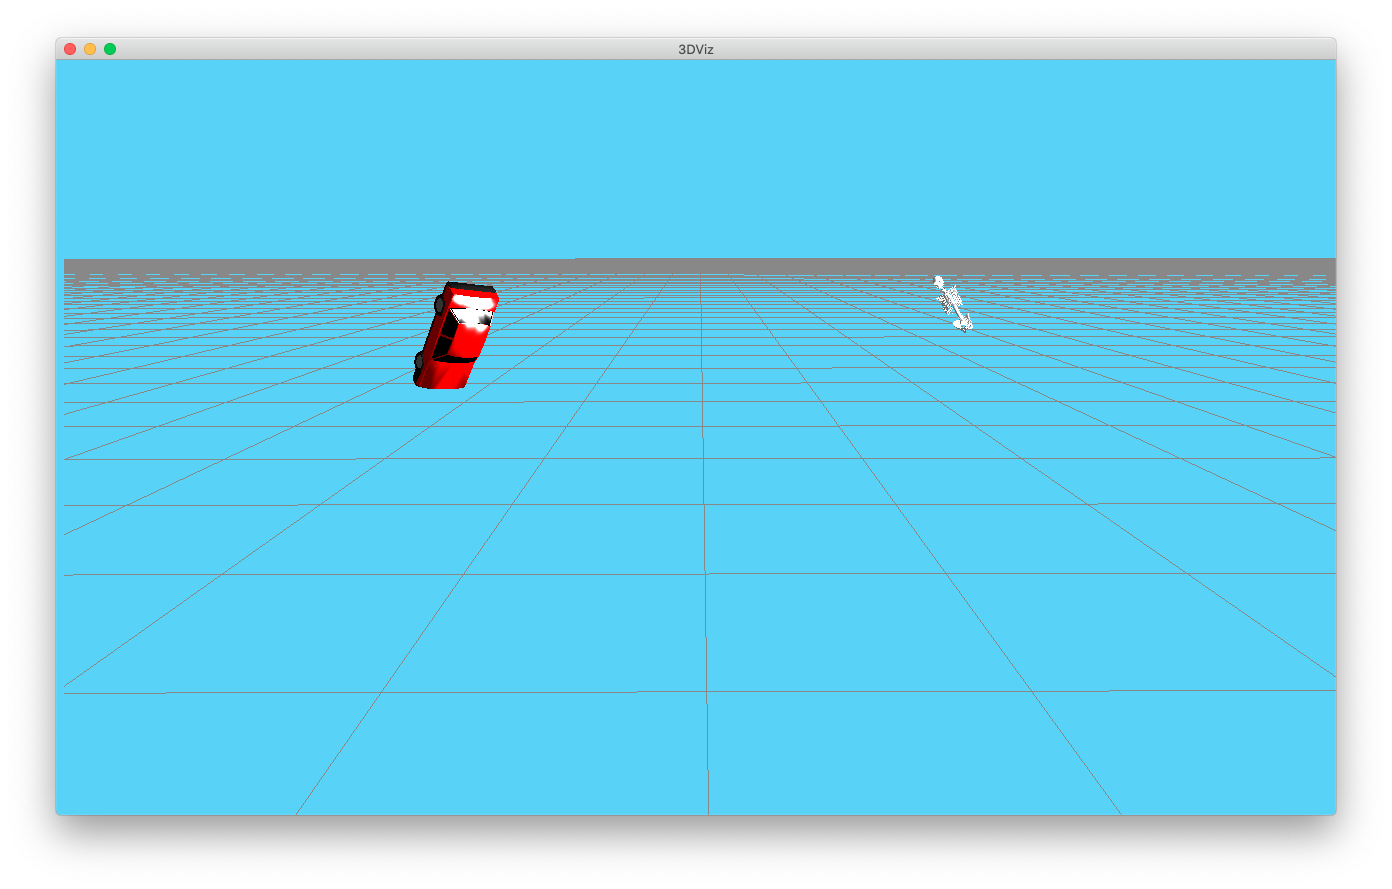
\includegraphics[width=0.8\textwidth]{figures/movermodelos.png}
		\caption{Objetos 3D reubicados y rotados}
		\label{fig.movermodelos}
		\end{center}
\end{figure}
\subsection{Borrado de elementos mostrados en el visor}
El visor ofrece dos posibilidades de borrado, la primera es borrado total de lo que se mostraba previamente en el visor, la segunda posibilidad es el borrado parcial del visor, de modo que solo se borra los elementos indicados por el servidor.
\begin{lstlisting}[caption= Código para realizar el borrado de elementos mostrados en el visor, label=cod.borrarelementos]
function deleteObj(id){
	if (id == ""){
		delete_list = id_list;
		id_list = ["points","line"];
		id_obj = [];
	} else if (id == "obj"){
		delete_list = id_obj;
		id_list = ["points","line"];
		id_obj = [];
	} else {
		delete_list = [id];
	}
	for (i = 0; i < id_list.length; i++){
		var selectedObject = scene.getObjectByName(delete_list[i]);
		while (selectedObject != null) {
			scene.remove(selectedObject);
			selectedObject = scene.getObjectByName(delete_list[i]);
		}
	}
}
\end{lstlisting}
El código del cuadro 5.8 primero verifica cual es el tipo de borrado, analizando la variable \texttt{id} que se pasa por parámetro. Si esta variable no tiene valor, el borrado es completo y la lista para borrar es la que contiene todos los identificadores de todos los elementos que se muestran en la escena, si toma el valor ``obj'' la lista apra borrar es la correspondiente a la que contiene los identificadores de los objetos 3D. Por último, si toma el valor ``line'' o ``points'', la lista esta formada únicamente por este identificador.

El borrado es selectivo, por lo que para realizarlo, previamente se debe haber identificado el elemento que se desea borrar y seleccionarlo en la escena mediante el identificador. Dado que la escena puede tener multiples elementos con el mismo identificador (los segmentos y los puntos), es necesario realizar varias iteraciones buscando los elementos de la escena que el identificador coincida con el deseado hasta eliminar todos los elementos de la escena que lo tienen, ya que la llamada a \texttt{getObjectByName} solo devuelve un elemento, y no todos.

\section{Estructura de los Mensajes}
En esta sección se describe la estructura de los mensajes que intercambian servidor y cliente para solicitar la visualización de cada tipo de primitiva 3D, ya sea punto, segmento u objeto. También como se definen utilizando el lenguaje de descripción Slice, explicado en el capitulo 3 de esta memoria. 
\subsection{Mensaje para visualizar los puntos}
Para representar un punto, como veremos en la siguiente sección, únicamente se necesita una posición en el eje de coordenadas y el color que tendrá el punto. Teniendo en cuenta esto, la estructura del mensaje es muy simple:
\begin{itemize}
\item Coordenada ``X''
\item Coordenada ``Y''
\item Coordenada ``Z''
\item Componente de color ``R'' (valor decimal entre 0 y 1)
\item Componente de color ``G'' (valor decimal entre 0 y 1)
\item Componente de color ``B'' (valor decimal entre 0 y 1)
\end{itemize}

Esta estructura es definida mediante el lenguaje Slice de la siguiente forma en el archivo ``primitives.ice'', que contiene las definiciones de las estructuras intermedias creadas para definir estructuras más complejas y definitivas:

\begin{lstlisting}[caption= Definición de la estrucutra del punto con Slice, label=cod.puntoslice]
#ifndef PRIMITIVES_ICE
#define PRIMITIVES_ICE

module jderobot{
	struct RGBPoint{
      		float x;
      		float y;
      		float z;
      		float r;
      		float g;
      		float b;
	};
};
#endif
\end{lstlisting}

Como se ha explicado anteriormente, el visor tiene la iniciativa y solicitará si hay nuevos puntos que mostrar cada cierto periodo de tiempo. Dado que puede interesar que este periodo sea largo para evitar constantes peticiones y mayor carga de trabajo, se ha decidido que no solo se pueda enviar un punto en cada petición, sino que se pueda enviar un buffer de puntos. La estructura del mensaje, por tanto, no es una posición en el eje de coordenadas y el color, sino una colección variable de estos elementos (podrá ser uno o más).

Para dar la posibilidad al servidor de indicar si desea añadir o eliminar lo que está pintado en ese momento en el visor (refrescar la escena que muestra el visor), al mensaje se le añade un parámetro que tome los valores ``all'', si se desea eliminar todo lo que se muestra en ese momento y únicamente que se visualice lo que se transmite en ese mensaje, ``part'', si lo que se desea es eliminar únicamente los elementos de este tipo y añadir los que se transmite en este mensaje al resto de elementos mostrados en la escena, o ``nothing'', si únicamente se desea añadir lo recibido sin eliminar nada de lo que está pintado en la escena.
Por tanto el mensaje quedará como sigue:
\begin{itemize}
\item Buffer de puntos con los siguientes parámetros:
	\begin{itemize}
	\item Coordenada ``X''
	\item Coordenada ``Y''
	\item Coordenada ``Z''
	\item Componente de color ``R'' (valor decimal entre 0 y 1)
	\item Componente de color ``G'' (valor decimal entre 0 y 1)
	\item Componente de color ``B'' (valor decimal entre 0 y 1)
	\end{itemize}
\item Refresco del visor
\end{itemize}

Esta estructura final del mensaje con el buffer de puntos y el refresco estará definida en el archivo Slice ``visualization.ice'', utilizando las primitivas creadas en el archivo ``primitives.ice'':

\begin{lstlisting}[caption= Definición del buffer de puntos con Slice, label=cod.bufferptoslice]
#ifndef VISUALIZATION_ICE
#define VISUALIZATION_ICE

#include <primitives.ice>

module jderobot{

	sequence<RGBPoint> Points;

	struct bufferPoints{
		Points buffer;
		string refresh;
	};
};
#endif
\end{lstlisting}


\subsection{Mensaje para visualizar segmentos}
Para visualizar un segmento únicamente es necesario enviar la posición en el eje de coordenadas de dos puntos y el color con el que se desea visualizar el segmento. Por tanto, la estructura del mensaje para representar un segmento es la siguiente:
\begin{itemize}
\item Punto de inicio
	\begin{itemize}
		\item Coordenada ``X''
		\item Coordenada ``Y''
		\item Coordenada ``Z''
	\end{itemize}
\item Punto de fin
	\begin{itemize}
		\item Coordenada ``X''
		\item Coordenada ``Y''
		\item Coordenada ``Z''
	\end{itemize}
\item Componente de color ``R'' (valor decimal entre 0 y 1)
\item Componente de color ``G'' (valor decimal entre 0 y 1)
\item Componente de color ``B'' (valor decimal entre 0 y 1)
\end{itemize}

Se extiende el archivo ``primitives.ice'' para incluir las estructuras intermedias necesarias:

\begin{lstlisting}[caption= Definición de la estrucutura del segmento con Slice, label=cod.segmentoslice]
structu Point{
	float x;
      	float y;
      	float z;
};

struct Segment{
	Point fromPoint;
	Point toPoint;
};


struct RGBSegment{
	Segment seg;
	float r;
	float g;
	float b;
};

\end{lstlisting}

Sin embargo, al igual que para el caso de los puntos, se desea poder enviar varios segmentos. El mensaje, por tanto, contiene un buffer de segmentos cuya estructura será una colección de dos puntos, con su posición en el eje de coordenadas, y el color de cada segmento.
Finalmente, también se incluye el parámetro para indicar si se debe refrescar el visor, ya sea completamente o parcialmente, o por el contrario simplemente añadir los segmentos enviados a lo que ya se muestra en la escena.
La estructura final del mensaje de envío de segmentos es la siguiente:
\begin{itemize}
	\item Buffer de segmentos
	\begin{itemize}
		\item Punto de inicio
		\begin{itemize}
			\item Coordenada ``X''
			\item Coordenada ``Y''
			\item Coordenada ``Z''
		\end{itemize}
		\item Punto de fin
		\begin{itemize}
			\item Coordenada ``X''
			\item Coordenada ``Y''
			\item Coordenada ``Z''
		\end{itemize}
		\item Componente de color ``R'' (valor decimal entre 0 y 1)
		\item Componente de color ``G'' (valor decimal entre 0 y 1)
		\item Componente de color ``B'' (valor decimal entre 0 y 1)
	\end{itemize}
	\item Refresco del visor
\end{itemize}

Ahora es necesario definir el formato definitivo del mensaje, para ello se extenderá el archivo ``visualization.ice'' de la siguiente forma:

\begin{lstlisting}[caption= Definición del buffer de segmentos con Slice, label=cod.buffersgmslice]
	
sequence<RGBSegment> Segments;
	
struct bufferSegments{
	Segments buffer;
	string refresh;
};
\end{lstlisting}

\subsection{Mensaje para visualizar un objeto 3D}
Mientras que para los segmentos y para los puntos únicamente se hace la petición sin añadir ningún parámetro a la misma (la forma de realizar la petición se detallará en secciones posteriores), en el caso de las peticiones de un objeto 3D desde el visor 3D al servidor, se le debe incluir el identificador que se le va a dar al objeto (en caso de que el servidor tenga uno para enviar), de modo que tanto visor como servidor pueden hacer corresponder las peticiones de movimiento o borrado con un objeto concreto mediante este identificador.

Para mostrar un objeto, se necesita conocer el archivo que contiene el objeto, el formato del archivo, la posición en el eje de coordenadas, la orientación del objeto y la escala del objeto. 
El archivo puede ser enviado de dos formas, la primera forma es mediante una URL a un servidor externo o página web, la segunda forma es enviar el fichero como texto plano. Esta segunda vía tiene el inconveniente de que no pueden ser enviados archivos de más de 1 MB de tamaño, por lo que si se quiere enviar un archivo más grande, debe realizarse mediante URL.

Se transmite también el formato del archivo, que como se ha explicado puede tomar los valores ``obj' o ``dae'', para que el visor pueda conocer el formato del objeto que se le está trasmitiendo y llamar a la función de procesamiento correspondiente.

La escala del objeto es un número decimal que indica el tamaño con el que se desea mostrar el objeto, permitiendo así mostrar varias veces el mismo objeto pero cambiando de tamaño (por ejemplo, podemos querer mostrar un brazo humano en diferentes tamaños para representar a un niño y a un adulto).

Por último, tanto para la posición como para la orientación se usará la clase ``Pose3D''. Esta clase esta formada por las coordenadas ``X'', ``Y'' y ``Z'', la coordenada homogénea ``h'', que no se utiliza, y los cuaterniones ``q0'', ``q1'', ``q2'' y ``q3'' para, usando las formulas matemáticas correspondientes, proporcionar la orientación del objeto.

El formato del mensaje tiene la siguiente estructura:
\begin{itemize}
	\item Archivo con el objeto 3D
	\item Formato del archivo
	\item	Pose3D
	\begin{itemize}
		\item Coordenada ``X''
		\item Coordenada ``Y''
		\item Coordenada ``Z''
		\item Coordenada homogénea``h''
		\item Cuaternión ``q0''
		\item Cuaternión ``q1''
		\item Cuaternión ``q2''
		\item Cuaternión ``q3''
	\end{itemize}
	\item Escala
	\item Identificador
	\item Refresco del visor
\end{itemize}
Como se puede ver, se vuelve a enviar el identificador que había sido previamente asignado y transmitido por el visor, y se añade también el refresco al igual que en los puntos y los segmentos. Sin embargo, debido a las limitaciones de tamaño de los archivos que se pueden enviar mediante ICE, y la necesidad de establecer un identificador común, solo es posible enviar un objeto 3D por petición realizada y no un buffer de objetos, como sí se puede hacer con los puntos y los segmentos.

La clase ``Pose3D'' es definida en un nuevo archivo Slice llamado ``pose3d.ice'':

\begin{lstlisting}[caption= Definición de la clase Pose3D con Slice, label=cod.pose3dslice]
#ifndef POSE3D_ICE
#define POSE3D_ICE

module jderobot{

  class Pose3DData
  {
		float x;
		float y;
		float z;
  		float h;
		float q0;
		float q1;
		float q2;
		float q3;
  };

}; 
#endif
\end{lstlisting}

Este mensaje queda definido en el archivo Slice ``visualization.ice'', al tratarse de un formato final y no de una primitiva (se trata de una estructura de mensaje final y no una estructura intermedia para crear nuevas). Además, es necesario incluir al principio la referencia al archivo `pose3d.ice'':

\begin{lstlisting}[caption= Definición de la estructura del objeto 3D con Slice, label=cod.obj3dslice]
#include <pose3d.ice>
	....
  	struct object3d {
    		string obj;
    		string id;
    		string format;
    		float scale;
    		Pose3DData pos;
    		string refresh;
  	};

 \end{lstlisting}


\subsection{Mensaje para mover los objetos 3D}
Los objetos 3D que se visualizan probablemente se desee moverlos de posición u orientación. Borrarlos y crearlos de nuevo implica un mayor retardo y carga de trabajo, por lo que ha sido necesario incorporar una secuencia de petición y envío de movimiento, pero solo se comenzará a realizar la petición de movimiento una vez se muestre un objeto ya en el visor. La estructura de este mensaje es una versión reducida del mensaje para crear un objeto. En este caso únicamente se deberá enviar la nueva posición mediante la clase ``Pose3D'' y el identificador del objeto que se desea mover. Por tanto, la estructura queda de la siguiente manera:
\begin{itemize}
	\item	Pose3D
	\begin{itemize}
		\item Coordenada ``X''
		\item Coordenada ``Y''
		\item Coordenada ``Z''
		\item Coordenada homogénea``h''
		\item Cuaternión ``q0''
		\item Cuaternión ``q1''
		\item Cuaternión ``q2''
		\item Cuaternión ``q3''
	\end{itemize}
	\item Identificador
\end{itemize}

Este mensaje queda definido en el archivo ``visualization.ice'', al tratarse de un movimiento y no de un elemento nuevo:

\begin{lstlisting}[caption= Definición de la estructura del movimiento de los objetos 3D con Slice, label=cod.movimientoslice]
struct PoseObj3D{
	Pose3DData pos;
	string id;
 };
\end{lstlisting}

Se puede enviar una secuencia de movimientos para uno o más objetos, por lo que, al no tener el impedimento del tamaño de los archivos o del identificador, se decide permitir el envío de buffers con estas secuencias de movimiento. Si entre petición y petición se ha movido por ejemplo un objeto real varias veces que se muestra en el visor, se puedan realizar esos movimientos al mismo tiempo en el visor, evitando largos retardos que provocarían enviar los movimientos de uno en uno. Como es evidente, en esta ocasión el campo refresco no se envíe al no tener sentido eliminar algo de lo que se muestra en la escena si estamos enviando la actualización de un elemento que se muestra en la escena. El \textit{timing} para actualizar el movimiento está establecido en el fichero de configuración del visor.
La estructura final del mensaje es la siguiente:
\begin{itemize}
	\item Buffer de movimientos
	\begin{itemize}
		\item	Pose3D
		\begin{itemize}
			\item Coordenada ``X''
			\item Coordenada ``Y''
			\item Coordenada ``Z''
			\item Coordenada homogénea ``h''
			\item Cuaternión ``q0''
			\item Cuaternión ``q1''
			\item Cuaternión ``q2''
			\item Cuaternión ``q3''
		\end{itemize}
		\item Identificador
	\end{itemize}
\end{itemize}

El mensaje final queda definido de la siguiente forma en el archivo ``visualization.ice'':

\begin{lstlisting}[caption= Definición del buffer de movimientos con Slice, label=cod.buffermovslice]
sequence<PoseObj3D> bufferPoseObj3D;
\end{lstlisting}

\section{Conexiones}
En esta sección se describe como se realiza la conexión y la posterior recepción de cada uno de los objetos y objetos 3D anteriormente indicados. La conexión se realiza mediante el middleware ICE y su lenguaje de especificación Slice nombrando a los ficheros creados con este lenguaje interfaces slice. Primero se detallará cómo se realiza la conexión con el servidor y la posterior petición de cada tipo de objeto. Finalmente, se explicará cómo se realiza la recepción de cada objeto y el tratamiento que recibe cada uno para su posterior visualización en el visor.

\subsection{Conexión y peticiones al servidor}
Para la conexión e intercambios con el servidor, el visor hace uso de los Web Workers de HTML5 \footnote{\url{https://www.w3schools.com/html/html5_webworkers.asp}} que permiten realizar ejecuciones en segundo plano sin bloquear al proceso principal. Su uso es imprescindible para que el hilo principal no se bloquee y pueda mostrar los elementos que se reciban mientras espera la recepción del resto de peticiones realizadas. En la figura 5.8 se muestra el esquema del funcionamiento del Worker:

\begin{figure}[H]
  \begin{center}
    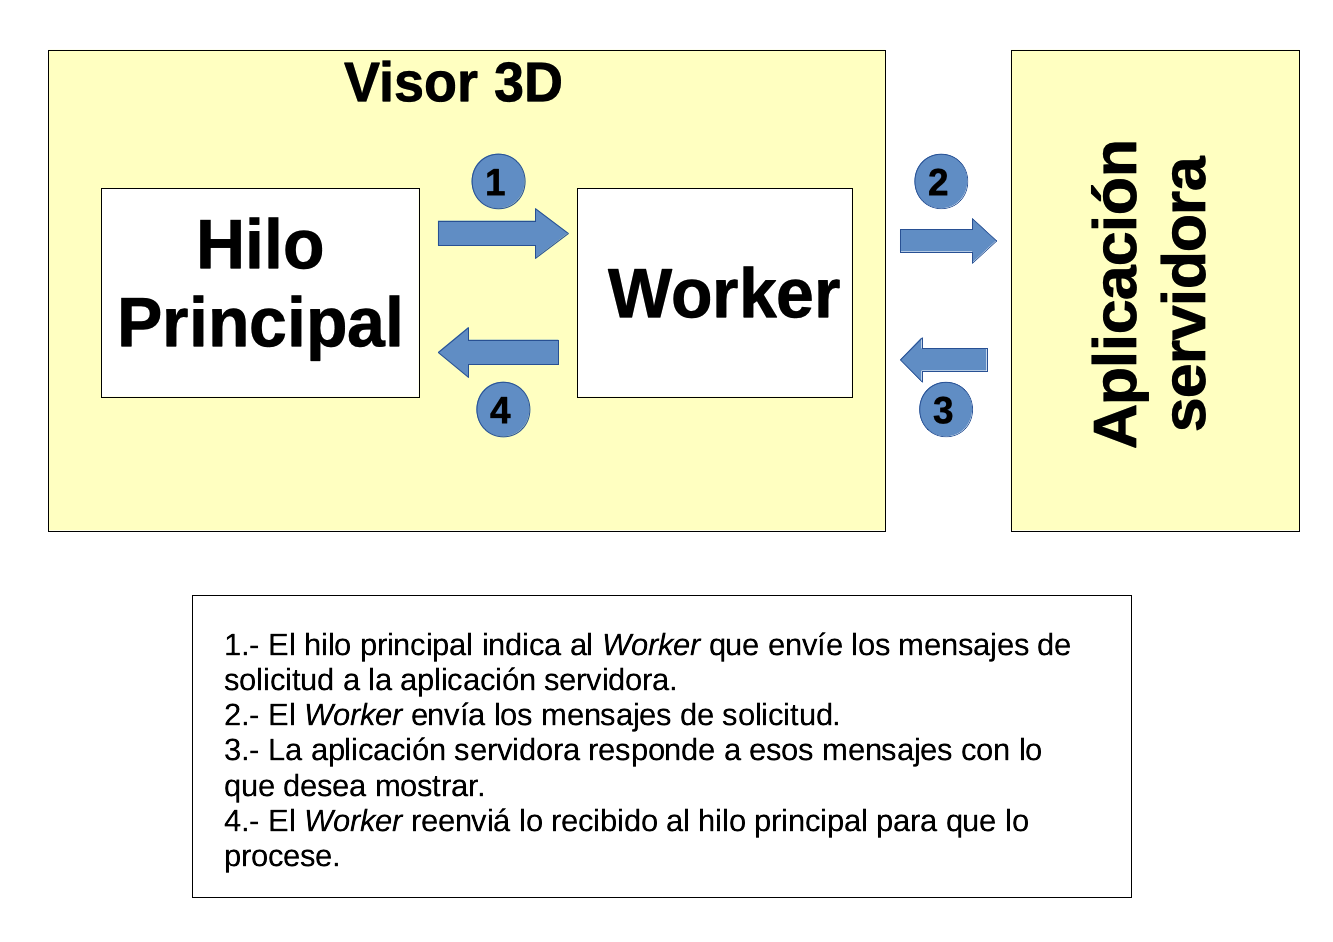
\includegraphics[width=0.8\textwidth]{figures/esquemaworker.png}
		\caption{Esquema de funcionamiento del Web Worker en el Visor 3D}
		\label{fig.diseno3dviz}
		\end{center}
\end{figure}

Una vez que el visor se ha lanzado y se ha terminado de cargar, se crea el Web Worker y se envía el mensaje para que se establezca la conexión. Esto se realiza utilizando el código del cuadro 5.17

\begin{lstlisting}[caption= Creación del Worker, label=cod.worker]
w = new Worker("js/3DViz_worker.js");
w.postMessage({func:"Start",server:config.Server, port:config.Port});
\end{lstlisting}

Cuando se ha creado el Worker se inicializa la conexión ICE que devuelve un objeto \texttt{Ice.Communicator}, que es el objeto principal para establecer una comunicación ICE. Posteriormente se crea un objeto con la interfaz indicada anteriormente para poder realizar la conexión. También se inicializan las variables para posteriormente lanzar el \textit{Promise} (permite manejar la naturaleza asíncrona de ICE) y la variable donde se guardará el \textit{proxy} con la conexión realizada con el servidor.
\begin{lstlisting}[caption= Código para la inicialización de la conexión ICE, label=cod.inicializarice]
var ic = Ice.initialize();
var communicator;
var Promise;
var Prx = jderobot.VisualizationPrx;
var srv;
\end{lstlisting}

Una vez incializada la conexión ICE, creado el objeto con la interfaz y recibido en el \textit{Worker} el mensaje para que se establezca la conexión, se comienza el proceso para realizarla. Lo primero que se debe realizar es crear el \textit{endpoint} mediante la ip y el puerto indicado en el fichero de configuración, después se crea un \textit{proxy} realizando una petición al servidor mediante la llamada a \texttt{stringToProxy}, pasándole como parámetro una cadena de texto que contiene la identidad del objeto (será a partir de la cual el servidor sea capaz de identificar a qué \textit{proxy} se está intentando conectar el cliente) y el \textit{endpoint}. El \textit{proxy} que nos devuelve es del tipo \texttt{Ice.ObjectPrx}, pero realmente lo que se necesita es un \textit{proxy} a la interfaz creada en ``visualization.ice'', que se hará mediante una petición \textit{Promise}, el objeto con la interfaz y el \textit{proxy} que se acaba de recibir. Esta petición lo que hace es preguntar al servidor si el \textit{proxy} que ha devuelto es un \textit{proxy} para el objeto de la interfaz de ``visualization.ice''. Si lo es devuelve un \textit{proxy} del tipo \texttt{jderobot.VisualizationPrx} que se guarda en la variable creada para almacenar la conexión. Si no devolverá un error.  Finalmente, el \textit{Worker} manda un mensaje al hilo principal indicando que la conexión se ha realizado correctamente.

\begin{lstlisting}[caption= Código para realizar la conexión ICE, label=cod.conexionice]
function connect(server,port){
  endpoint = "ws -h " + server + " -p " + port;
  var proxy = ic.stringToProxy("3DViz:" + endpoint);
  Promise = Prx.checkedCast(proxy).then(
      function(printer)
      {
          srv = printer;
          self.postMessage({func:"Connect"});
      });
}
\end{lstlisting}

Cuando el hilo principal recibe el mensaje indicando que la conexión ha sido exitosa establece las llamadas periódicas (utilizando el tiempo indicado en el fichero de configuración) a las funciones que se encargan de realizar las peticiones al servidor mediante el método de HTML \texttt{setInterval()} \footnote{\url{https://www.w3schools.com/jsref/met_win_setinterval.asp}}. Si no lo ha sido elimina el \textit{Worker} e imprime el mensaje por consola. 

\begin{lstlisting}[caption= Código para crear las llamadas periódicas a las funciones encargadas de realizar las peticiones al servidor, label=cod.funcionesinterval]
w.onmessage = function(event) {
      	 if (event.data.func == "Connect"){
		pointInterval = setInterval(function(){
					setPoint();
						}, config.updatePoints);
		lineInterval = setInterval(function(){
					setLine();
					},config.updateSegments);
		objInterval = setInterval(function(){
					setObj();
					},config.updateModels);}	
        } else {
          console.log(event.data);
          w.terminate();
        }
\end{lstlisting}

Cuando se pase el tiempo, se activan las funciones que envían el mensaje al \textit{Worker} para que realice las peticiones al servidor. Estas peticiones serán para todos los objetos igual salvo en el caso de la petición de los objetos 3D, que como se ha explicado anteriormente, enviará el identificador que se dará al objeto en caso de que haya uno. Este identificador será una cadena de ``obj'' y un contador de objetos que hay en la escena, es decir, si no hay objetos en la escena, el siguiente tendrá de identificador ``obj1'', el siguiente ``obj2'' y así sucesivamente. Finalmente, esta función termina realizando una llamada a la función que se encargará de gestionar las respuestas del servidor.

\begin{lstlisting}[caption= Definición de las funciones de petición, label=cod.funcionespeticion]
function setPoint(){
      w.postMessage({func:"setPoint"});
      getData();
}
function setLine(){
	w.postMessage({func:"setLine"});
	getData();
}
function setObj(){
	id = "obj" + cont;
	w.postMessage({func:"setObj", id: id});
	getData();
}
\end{lstlisting}

En el \textit{Worker}, cuando se reciban los mensajes que solicitan pintar cada tipo de elemento al servidor, se realiza la petición usando el proxy con la conexión y las funciones definidas en la interfaz Slice explicada anteriormente. Si a la petición se recibe respuesta, se reenvía al hilo principal para su manejo.

\begin{lstlisting}[caption= Código que realiza las peticiones al servidor, label=cod.peticiones]
function setPoint(point){
 	srv.getPoints().then(function(data){
		self.postMessage({func:"drawPoint",points: data});
	});
}

function setLine(){
	srv.getSegment().then(function(data){
      		self.postMessage({func:"drawLine", segments: data});
  	});
}

function setObj(id){
  	srv.getObj3D(id).then(function(data){
    		self.postMessage({func:"drawObj", obj: data});
  	});
}
\end{lstlisting}

Como se puede ver, solo se están realizando las peticiones para los puntos, los segmentos y los objetos, pero no para los movimientos de los objetos, ya que solo se realiza una vez que se ha recibido un objeto para mostrar. Una vez que se tiene un objeto, se activa la llamada periódica a la función para que envíe el mensaje al \textit{Worker} para que se realice la petición al servidor de la misma forma que las demás.

Las funciones para realizar las peticiones al servidor se han tenido que definir previamente mediante el lenguaje de descriptivo de ICE, Slice. Para realizar la definición se ha extendido el archivo ``visualization.ice'' explicado en la sección 5.4. A este archivo se le añade la descripción del cuadro 5.23.

\begin{lstlisting}[caption= Código añadido a las definiciones Slice creadas, label=cod.extensionslice]
interface Visualization
	{
	      bufferSegments getSegment ();
	      bufferPoints getPoints();
	      object3d getObj3D(string id);
	      bufferPoseObj3D getPoseObj3DData();
	};
};

\end{lstlisting}

\subsection{Recepción y tratamiento de los mensajes recibidos}
Ya se ha explicado cómo se conecta, se envían los mensajes de petición al servidor y se recepciona la respuesta en el Worker que la transmite al hilo principal. Ahora se explicará cómo trata esos mensajes el hilo principal para mostrarlo en el visor.

En el hilo principal hay un manejador de mensajes que es la función \texttt{getData()}, se invoca cada vez que se realiza una petición. En esta función se analiza el mensaje que se recibe procedente del \textit{Worker}. Se revisa cuál es el tipo y se realizan las tareas previas necesarias para posteriormente visualizar el elemento usando los métodos explicados en la sección sobre la interfaz gráfica. El condicional que se muestra en el cuadro 5.24 es el encargado de realizar este análisis.

\begin{lstlisting}[caption= Manejador que analiza los mensajes recibidos, label=cod.manejador]
function getData (){
	w.onmessage = function(event) {
		if (event.data.func == "drawPoint"){
			...
		} else if (event.data.func == "drawLine"){
			...
		} else if (event.data.func == "drawObj") {
			...
		} else if (event.data.func == "pose3d") {
			...
		}
	}
}
\end{lstlisting}

\subsubsection{Tratar los puntos}
Si el mensaje enviado por el \textit{Worker} es del tipo \texttt{drawPoint}, el manejador indicará que se deben ejecutar las sentencias correspondientes a la visualización de los puntos. Una vez concluido que se deben mostrar los puntos, lo primero que se realiza es verificar si el servidor ha solicitado que haya refresco del visor total, parcial o que no haya refresco, si el servidor ha indicado que se debe refrescar el visor (y si el mensaje trae puntos que mostrar, ya que si no se interpretará el mensaje como erróneo), se llama al método encargado de eliminar todos o algunos de los elementos que se muestran en ese momento en el visor y que se explica en la sección 5.3.5. 

Tanto si se ha refrescado como si no, se recorre el buffer de puntos mediante un bucle \texttt{for}, invocando al método encargado de mostrar un punto en el visor, en cada iteración hasta que ya no queden más puntos para mostrar. Al método se le pasa por parámetros el punto completo (coordenadas y componentes RGB), ya que se encarga de diferenciar cada uno y realizar las tareas necesarias para mostrarlos. 

\begin{lstlisting}[caption= Código para tratar los mensajes con los puntos, label=cod.tratarpuntos]
if (event.data.func == "drawPoint"){
	if (event.data.points.buffer.length !=0){
		if (event.data.points.refresh == "all"){
			deleteObj("");
		} else if ((event.data.points.refresh == "part")) {
			deleteObj("points");
		}
	}
	points = event.data.points.buffer;
	for (var i = 0; i < points.length; i+=1) {
        		addPoint(points[i]);
	}
}
 \end{lstlisting}

\subsubsection{Tratar los segmentos}
El tratamiento de los mensajes que contienen los segmentos es muy similar al de los mensajes con los puntos. Se revisa si es necesario refrescar el visor o no, si así lo fuera se eliminan total o parcialmente los elementos que hay en el visor, posteriormente se recorre el buffer de segmentos mediante el bucle \texttt{for} y finalmente se llama al método para mostrar segmentos en cada iteración. Al igual que en el caso de los puntos, se pasa como parámetro el array de segmentos completos y ya se encarga el método de separarlos y realizar las tareas correspondientes.

\begin{lstlisting}[caption= Código para tratar los mensajes con los segmentos, label=cod.tratarsegmentos]
else if (event.data.func == "drawLine"){
	if (event.data.segments.buffer.length !=0){
		if (event.data.segments.refresh == "all"){
			deleteObj("");
		} else if ((event.data.segments.refresh == "part")) {
			deleteObj("line");
		}
	}
	segments = event.data.segments.buffer;
	for (var i = 0; i < segments.length; i+=1) {
		addLine(segments[i], "segments");
	}
}
\end{lstlisting}

\subsubsection{Tratar los objetos 3D}
El tratamiento de los objetos 3D comienza de la misma forma revisando si requiere refresco, o no, del visor. Sin embargo, una vez que se ha borrado, o no, el contenido del visor, se actualiza el contador que constituye el identificador que se ha indicado en las secciones anteriores. Posteriormente es necesario realizar la conversión de la ubicación y orientación enviada como ``Pose3D'' a un formato que el método encargado de mostrar los objetos sea capaz de entender.

Para realizar esta conversión, lo primero es crear una clase de JavaScript cuya estructura contendrá los parámetros que se necesitan para mostrar el objeto, es decir la posición en el eje de coordenadas (coordenadas ``x'', ``y'' y ``z''), las orientaciones en cada eje de coordenadas (orientación ``rx'', ``ry'' y ``rz'') y el identificador del objeto 3D.
\begin{lstlisting}[caption= Definición de la clase que proporciona la posición de un objeto 3D, label=cod.clasepos]
class obj3DPose {
	constructor(id, x, y, z, rx, ry, rz){
		this.id = id;
		this.x = x;
		this.y = y;
		this.z = z;
		this.rx = rx;
		this.ry = ry;
		this.rz = rz;
	}
}
\end{lstlisting}

Para realizar la conversión se han creado tres métodos diferentes que devolverán cada uno de ellos la orientación en cada uno de los ejes de coordenadas. Estos métodos usan las formulas matemáticas que transforman los cuaterniones en los ángulos usados para describir la orientación de un objeto tridimensional y que son un tipo de ángulos de Euler \footnote{\url{https://en.wikipedia.org/wiki/Conversion_between_quaternions_and_Euler_angles}}. Este sistema es muy utilizado en navegación de los aviones y drones, y están formados por la dirección (``yaw''), elevación (``pitch'') y ángulo de alabeo (``roll'') correspondiendo respectivamente a la orientación en el eje ``z'', el eje ``y'' y el eje ``z''. Estas formulas matemáticas incorporadas a nuestro código originan los métodos que se muestran en el cuadro 5.28.

\begin{lstlisting}[caption= Funciones para realizar la conversión de la orientación, label=cod.conversionpose3d]

function getYaw(q0,q1,q2,q3) {
       var rotateZa0=2.0*(q1*q2 + q0*q3);
       var rotateZa1=q0*q0 + q1*q1 - q2*q2 - q3*q3;
       var rotateZ=0.0;
       if(rotateZa0 != 0.0 && rotateZa1 != 0.0){
           rotateZ=Math.atan2(rotateZa0,rotateZa1);
       }
       return rotateZ;
}

function getRoll(q0,q1,q2,q3){
       rotateXa0=2.0*(q2*q3 + q0*q1);
       rotateXa1=q0*q0 - q1*q1 - q2*q2 + q3*q3;
       rotateX=0.0;

       if(rotateXa0 != 0.0 && rotateXa1 !=0.0){
           rotateX=Math.atan2(rotateXa0, rotateXa1);
       }
       return rotateX;
}
function getPitch(q0,q1,q2,q3){
       rotateYa0=-2.0*(q1*q3 - q0*q2);
       rotateY=0.0;
       if(rotateYa0>=1.0){
           rotateY=Math.PI/2.0;
       } else if(rotateYa0<=-1.0){
           rotateY=-Math.PI/2.0
       } else {
           rotateY=Math.asin(rotateYa0)
       }

       return rotateY;
}
\end{lstlisting}

Finalmente se crea una función que devuelve un objeto de la nueva clase creada y que tiene ya la conversión. A esta función se le pasa por parámetro el objeto completo recibido y, mediante la llamada a las funciones para realizar la conversión, crea el objeto de la nueva clase que contendrá el identificador, las coordenadas ``x'', ``y'' y ``z'', sin ningún tipo de conversión, y las orientaciones en cada eje convertidas y que están en radianes.

\begin{lstlisting}[caption= Función que devuelve la posición tras la conversión, label=cod.posicionconvertida]
function getPose3D(data){
	var rotateZ=getYaw(data.pos.q0, data.pos.q1, data.pos.q2, data.pos.q3);
	var rotateY=getPitch(data.pos.q0, data.pos.q1, data.pos.q2, data.pos.q3);
	var rotateX=getRoll(data.pos.q0, data.pos.q1, data.pos.q2, data.pos.q3);
	var objpose3d = new obj3DPose(data.id, data.pos.x, data.pos.y,
						data.pos.z, rotateX, rotateY, rotateZ);
	return objpose3d;
}
\end{lstlisting}

Una vez que ya hemos realizado la conversión se llama al método encargado de cargar los objetos en el visor y que se explicó en la sección correspondiente. A este método, se le pasa por parámetro el objeto completo recibido del servidor y el objeto de la nueva clase que incorpora la conversión de la orientación, para que pueda mostrar el objeto en el visor. Tras ello, se arranca la petición periódica de movimientos para el objeto (si no estaba arrancada previamente) al tener ya mínimo un objeto para mover.

\begin{lstlisting}[caption= Código para tratar los mensajes con el objeto 3D, label=cod.tratarobjetos]
else if (event.data.func == "drawObj") {
	if (event.data.obj.obj !=""){
		if (event.data.obj.refresh == "all"){
			deleteObj("");
		} else if ((event.data.obj.refresh == "part")) {
			deleteObj("obj");
		}
	}
	cont += 1
	var pos = getPose3D(event.data.obj);
	addObj(event.data.obj,pos);
	if (posInterval == null){
		posInterval = setInterval(function(){
			setPose3D();
		}, config.updatePose3D);
	}
}	
\end{lstlisting}

\subsubsection{Tratar el movimiento de los objetos}
En el caso de los mensajes con el movimiento únicamente se recorrerá buffer que contiene todos los movimientos realizando la conversión de Pose3D al formato admitido explicado anteriormente e invocando al método que realiza el movimiento de los objetos explicado en la sección sobre la interfaz gráfica. 

En la clase que se ha creado para la conversión se incluye el identificador del objeto que se va a mover, ya que, a diferencia de cuando invocamos al método que representa el objeto en el visor que se pasaba por parámetro el mensaje completo recibido del servidor y la nueva clase, en este caso solo pasamos por parámetro la nueva clase por lo que es necesario incluir el identificador.

\begin{lstlisting}[caption= Código para tratar los mensajes con los movimientos de los objetos 3D, label=cod.tratarmovimiento]
else if (event.data.func == "pose3d") {
	for (var i = 0; i < event.data.bpose3d.length; i += 1){
		data = event.data.bpose3d[i];
		var objpose3d = getPose3D(data);
		moveObj(objpose3d);}
	}
}
\end{lstlisting}

\section{Experimentos}
El visor está preparado para ser usado principalmente con Electron, ya que la lectura del fichero de configuración solo esta habilitada para sí se usa con Electron. Se puede utilizar en el navegador web, pero la configuración será la que se indica al visor por defecto, no pudiendo modificarse, lo que limita en gran manera las funciones del mismo. La ejecución con Electron se realiza de la misma manera que se explicó en la sección 3.8.

Para ejecutar el visor 3D y realizar pruebas, se ha creado un servidor de test escrito en python que enviará todos los tipos de elementos y movimientos, enviando valores aleatorios. En cada mensaje envía entre 1 y 5 puntos y rectas, está preparado para enviar 3 objetos (uno en forma de texto plano y dos desde una URL) y movimientos aleatorios para esos objetos.

\begin{enumerate}
\item En un terminal ejecutar el servidor de prueba:
\begin{lstlisting}[caption= Ejecutar servidor de prueba, label=cod.testserver]
python server_test.py
\end{lstlisting}
\item En otro terminal, instalar Electron y las dependencias del visor:
\begin{lstlisting}[caption= Instalar Electron y sus dependencias, label=cod.instalarelectron]
npm install
\end{lstlisting}
\item En el mismo terminal, ejecutar el visor 3D con Electron:
\begin{lstlisting}[caption= Ejecutar el visor 3D mediante Electron, label=cod.tratarobjetos]
npm start
\end{lstlisting}
\end{enumerate}

A continuación se muestra la prueba realizada con el servidor, tomando varias secuencias del mismo experimento:

\begin{figure}[H]
  \begin{center}
    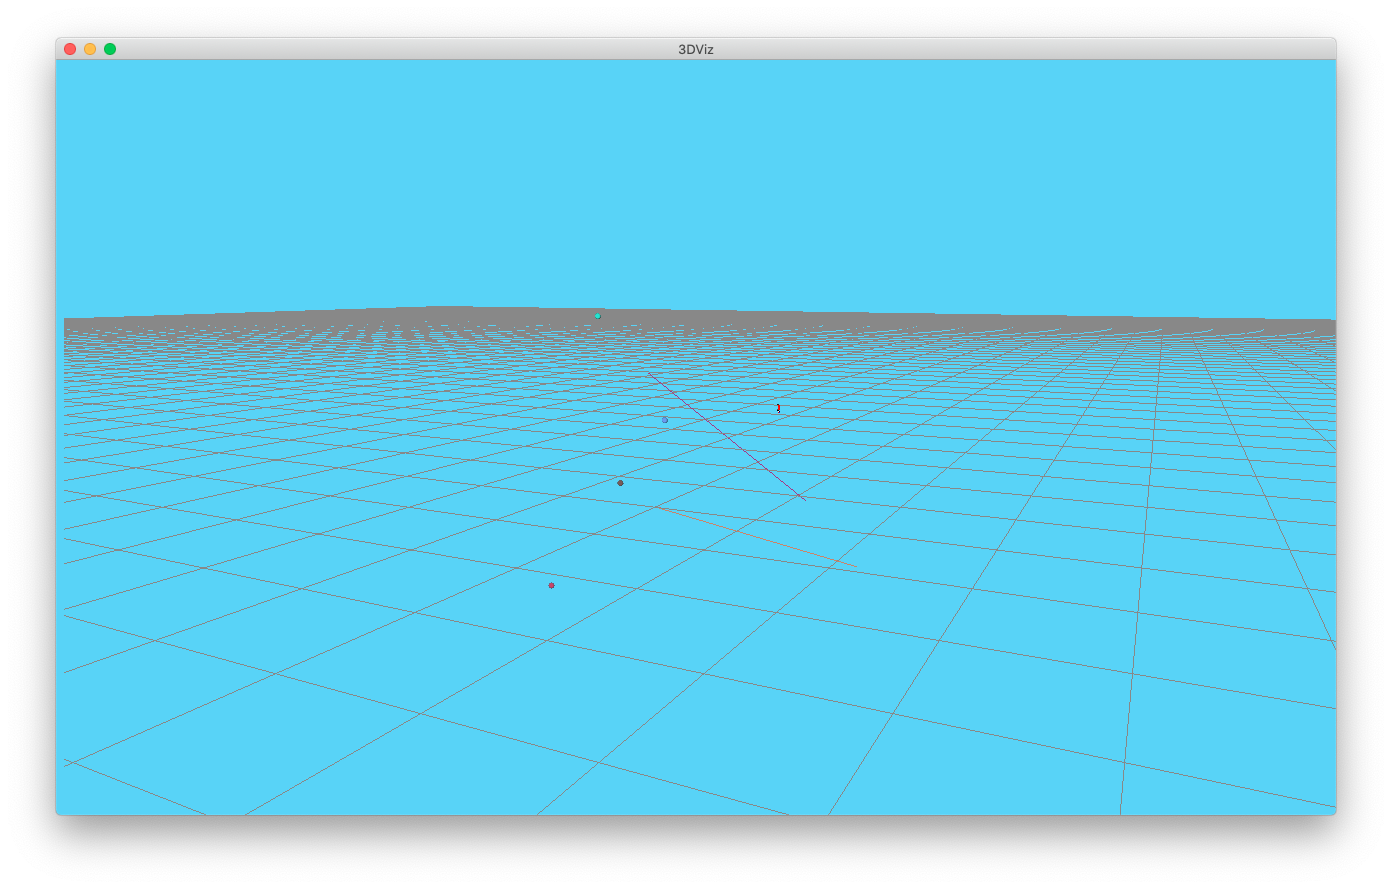
\includegraphics[width=0.8\textwidth]{figures/test3dviz1.png}
		\label{fig.test3dviz1}
		\end{center}
\end{figure}
\begin{figure}[H]
  \begin{center}
    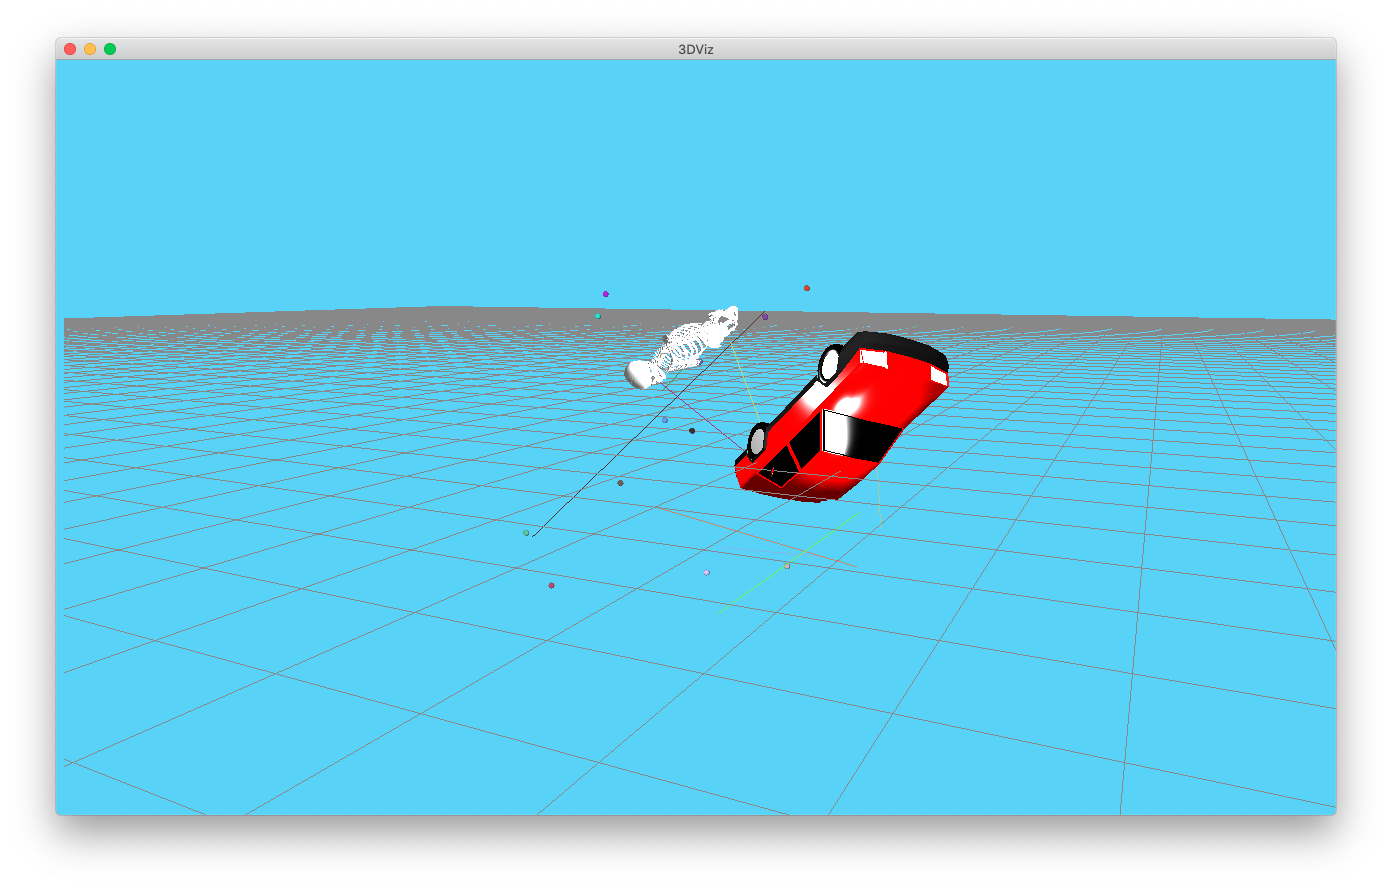
\includegraphics[width=0.8\textwidth]{figures/test3dviz2.png}
		\label{fig.test3dviz2}
		\end{center}
\end{figure}
\begin{figure}[H]
  \begin{center}
    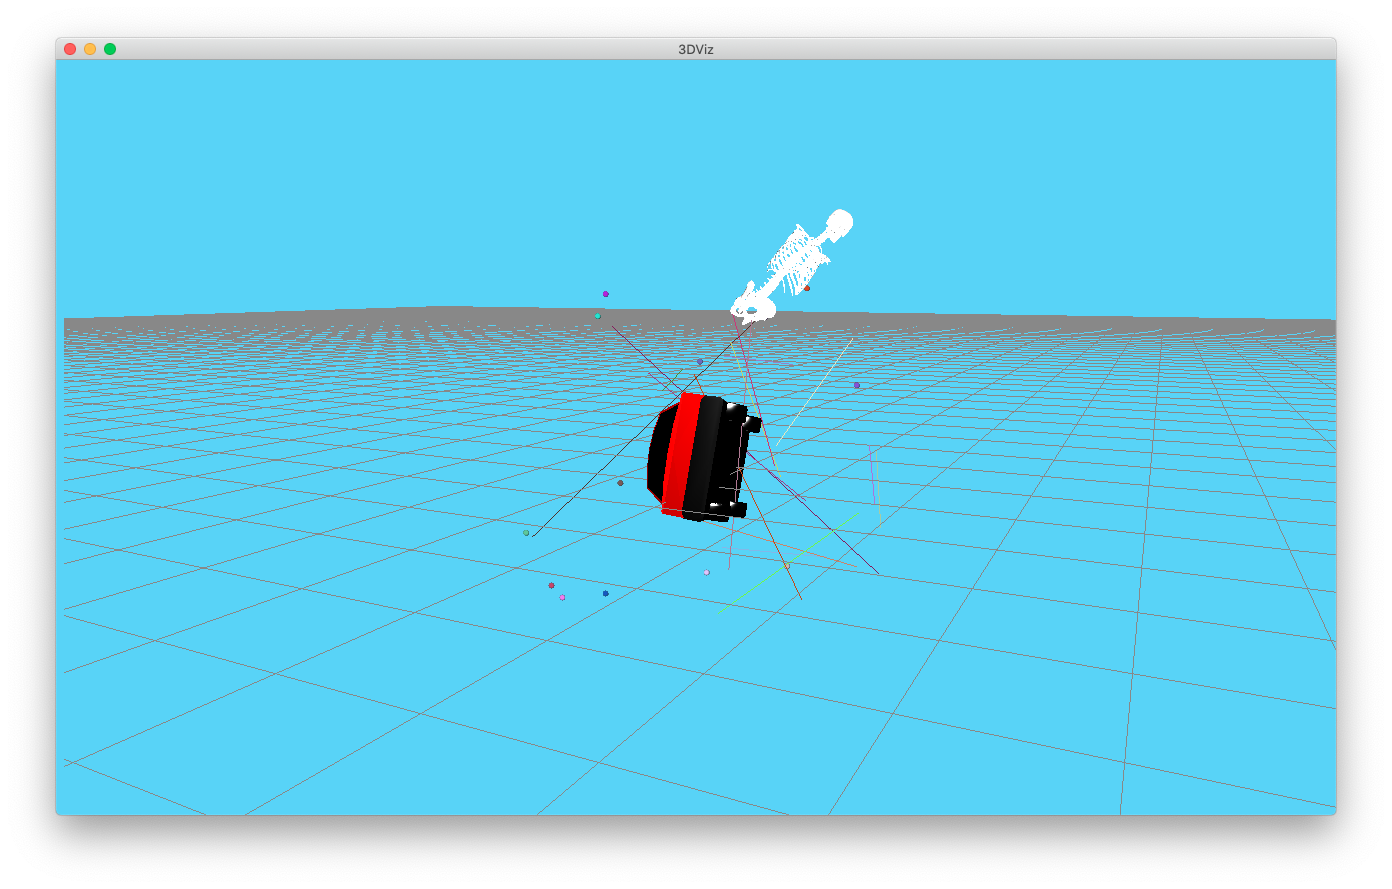
\includegraphics[width=0.8\textwidth]{figures/test3dviz3.png}
		\label{fig.test3dviz3}
		\caption{Secuencias de imágenes tomadas del experimento}
		\end{center}
\end{figure}
\begin{figure}[H]
  \begin{center}
    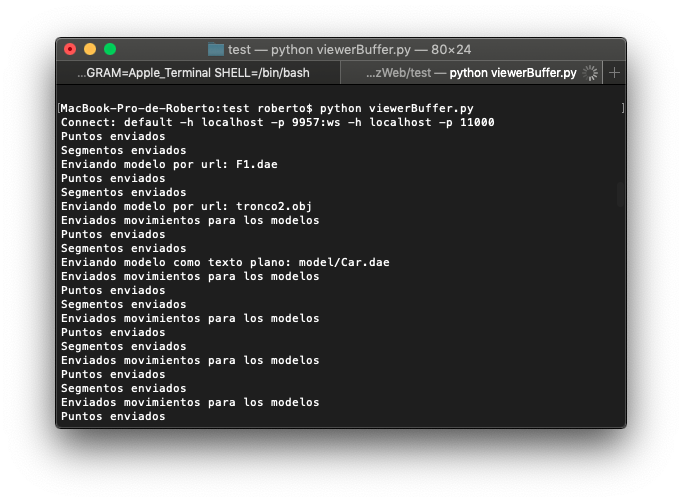
\includegraphics[width=0.8\textwidth]{figures/servertest3dviz.png}
		\label{fig.servertest3dviz}
		\caption{Aplicación servidora de prueba}
		\end{center}
\end{figure}














\lhead[]{CAP\'ITULO \thechapter. CAMSERVER}
\chapter{Servidor de imágenes con tecnologías web }\label{cap.camserver}
En este capítulo expondrá la creación de un nuevo driver para la plataforma JdeRobot. Este driver es un servidor de imágenes, al que se ha llamado CamServerWeb, obtenidas mediante una webcam (ya sea externa o interna del ordenador) de modo que cualquier aplicación externa pueda obtener las imágenes obtenidas.
\section{Diseño}
Este driver está diseñado con JavaScript y HTML como lenguajes de programación, y ROS como middleware para la interconexión con los diferentes clientes. El driver puede ser ejecutado como una aplicación de escritorio usando el framework Electron o como una página web usando un navegador. Gracias a esto, se permite la ejecución multiplataforma sin necesidad de realizar modificaciones, lo que provee a este driver de una gran ventaja respecto a los tradicionales, que se tenían que están desarrollados para una única plataforma.  En la figura 6.1 se muestra el esquema de funcionamiento del driver.
\begin{figure}[H]
  \begin{center}
    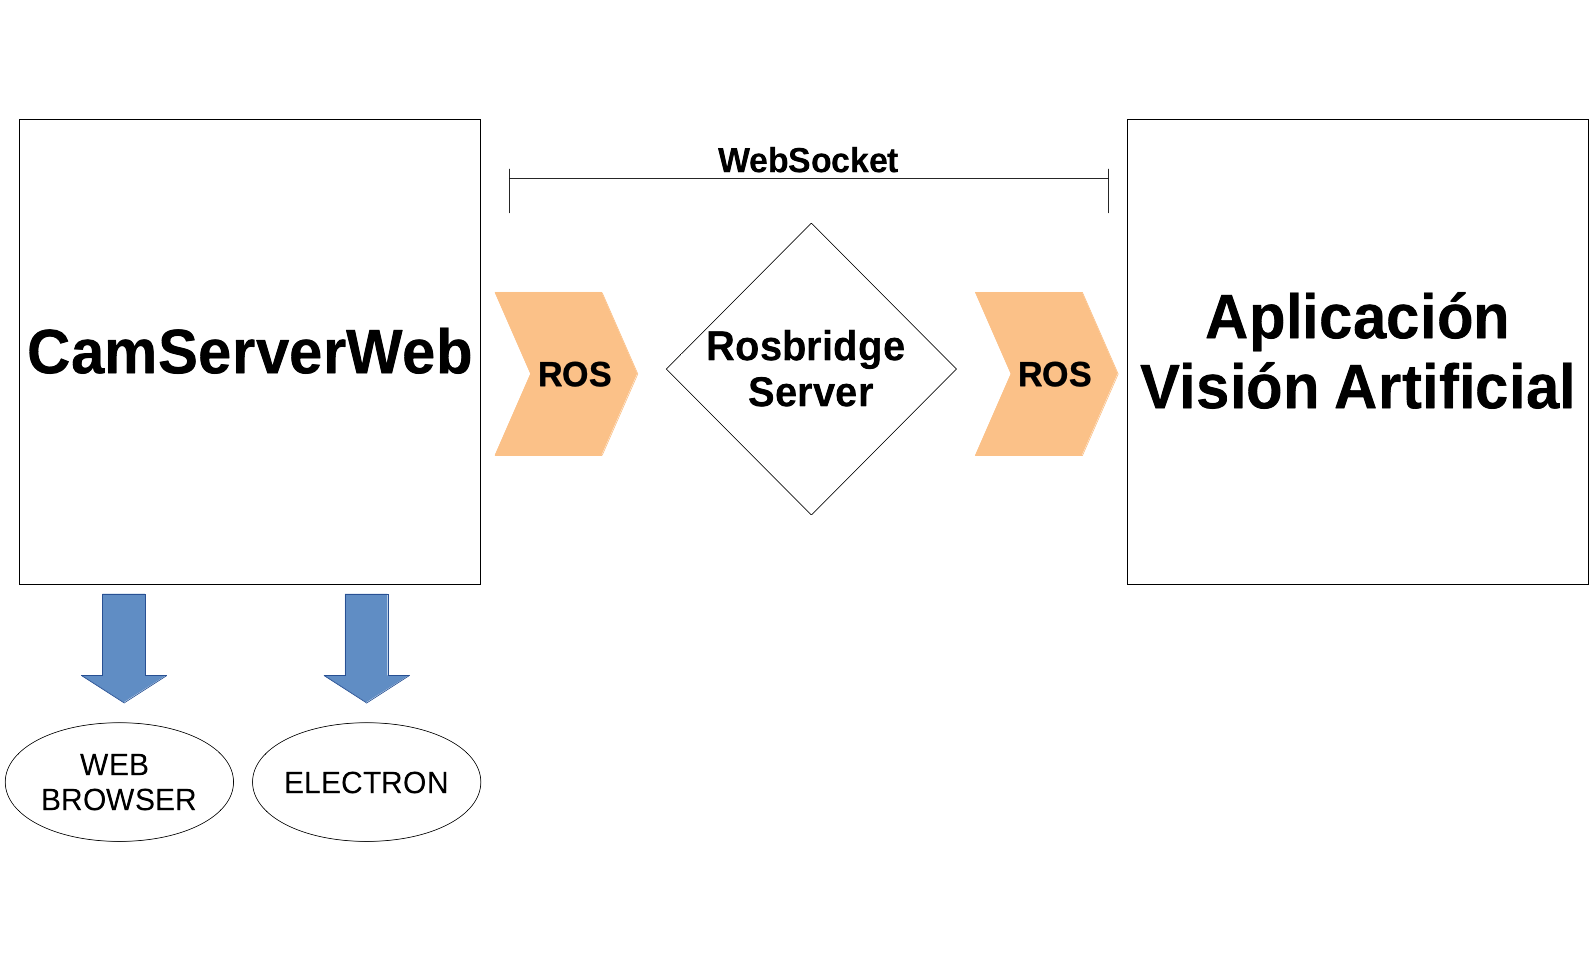
\includegraphics[width=0.8\textwidth]{figures/cajanegracamserver.png}
		\caption{Diseño del driver CamServerWeb}
		\label{fig.diseñocamserver}
		\end{center}
\end{figure}

Se puede apreciar en el esquema, que entre el driver y la aplicación de visión artificial hay un servidor intermedio. Este servidor proporciona una capa de transporte WebSocket para realizar la conexión con una aplicación web. En este caso permite la comunicación entre el servidor de imágenes y la aplicación de visión artificial que desea obtener las imágenes.

El driver cuenta con dos partes bien diferenciadas. La primera parte corresponde a la adquisición de las imágenes usando WebRTC para realizar la conexión con la fuente de video, y la segunda parte es la encargada de realizar la conexión mediante ROS y el posterior envío de los mensajes mediante los \textit{Publisher} de ROS para que sean recibidos por la aplicación de visión artificial que desea obtener las imágenes. Gracias al uso de ROS, se posibilita que la aplicación de visión artificial esté desarrollada en cualquier lenguaje de programación y ejecutada en cualquier dispositivo ubicado en cualquier lugar del mundo. Finalmente, el driver cuenta de una interfaz gráfica de apoyo para poder realizar la configuración en tiempo de ejecución. Esta estructura se puede observar en la figura 6.2.
\begin{figure}[H]
  \begin{center}
    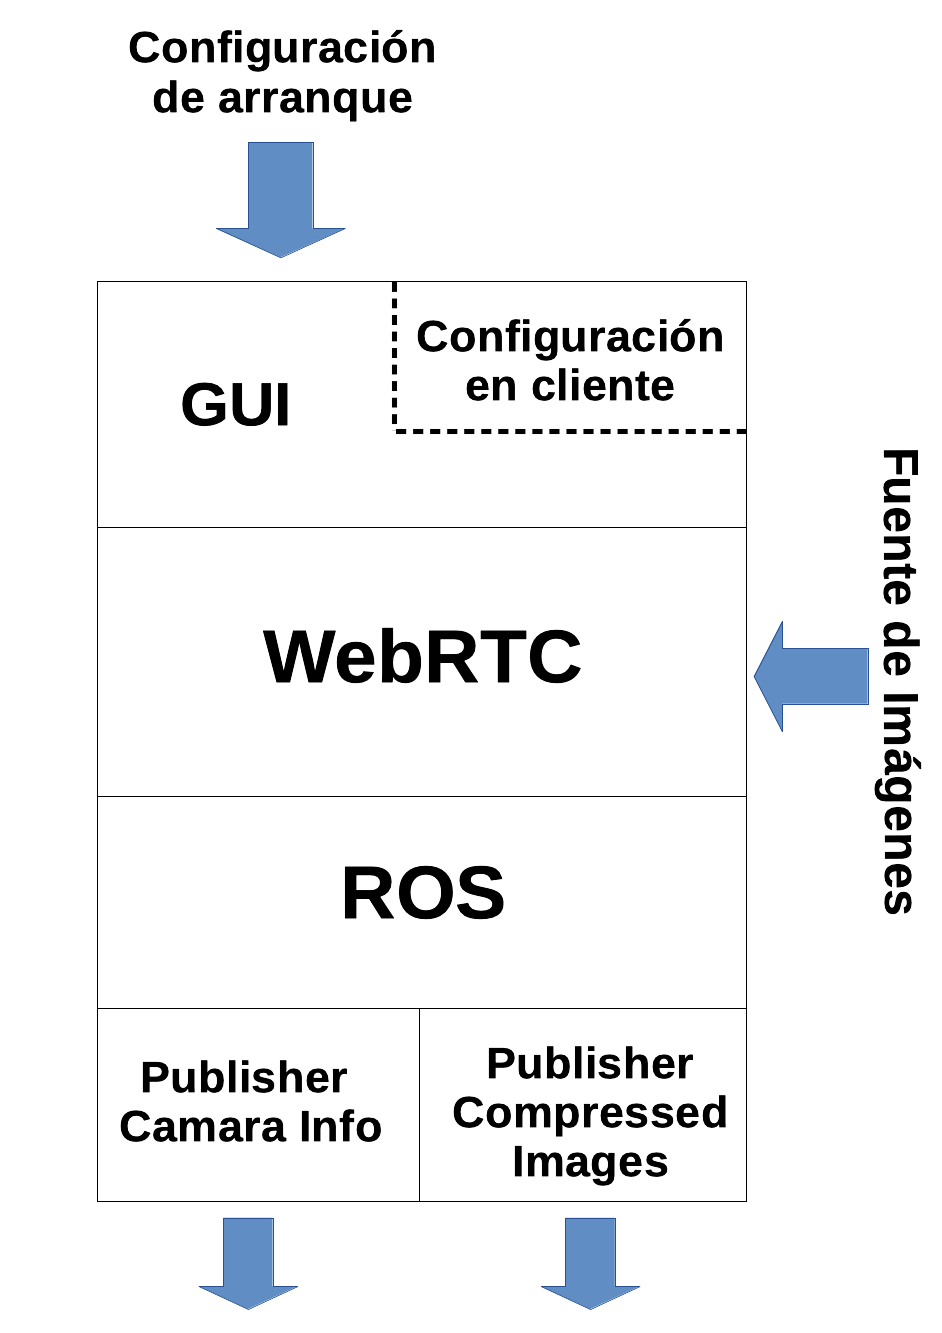
\includegraphics[width=0.8\textwidth]{figures/cajablancacamserver.png}
		\caption{Estructura interna de CamServerWeb}
		\label{fig.estructuracamserver}
		\end{center}
\end{figure}

\section{Adquisición y preparación de imágenes}
Para la obtención de las imágenes se hace uso del proyecto de código abierto WebRTC, que permite la transmisión en tiempo real de audio, video y datos.
Mediante WebRTC se obtienen las imágenes de una cámara utilizando muy pocas línea de código, lo que facilita enormemente el trabajo. El único problema que se ha tenido que tener en cuenta y solucionar, es el formato en el que se obtienen esas imágenes que es incompatible con ROS, por lo que se han tenido que llevar a cabo modificaciones en el formato de la imagen.

Lo primero que se debe realizar es recopilar todos los dispositivos conectados al ordenador y separar los dispositivos de video, que son los que realmente interesan. Para lograrlo, se utiliza el api \texttt{Navigator} de WebRTC, proporcionándonos el objeto \texttt{navigator.mediaDevices}, al cual si le añadimos \texttt{.enumerateDevices().then(function (devices)\{\})}, obtenemos todos los dispositivos multimedia conectados al ordenador donde se está ejecutando. Una vez que ya se tienen todos los dispositivos, simplemente interesan, aquellos capturadores de video, es decir, serán aquellos dispositivos cuyo tipo es de entrada de video (en nuestro código sería un condicional \texttt{if (devices.kind == "videoinput")\{\})}. La lista de dispositivos se muestra en el menu de configuración, mediante un campo desplegable como se muestra en la figura 6.3.
 \begin{figure}[H]
  \begin{center}
    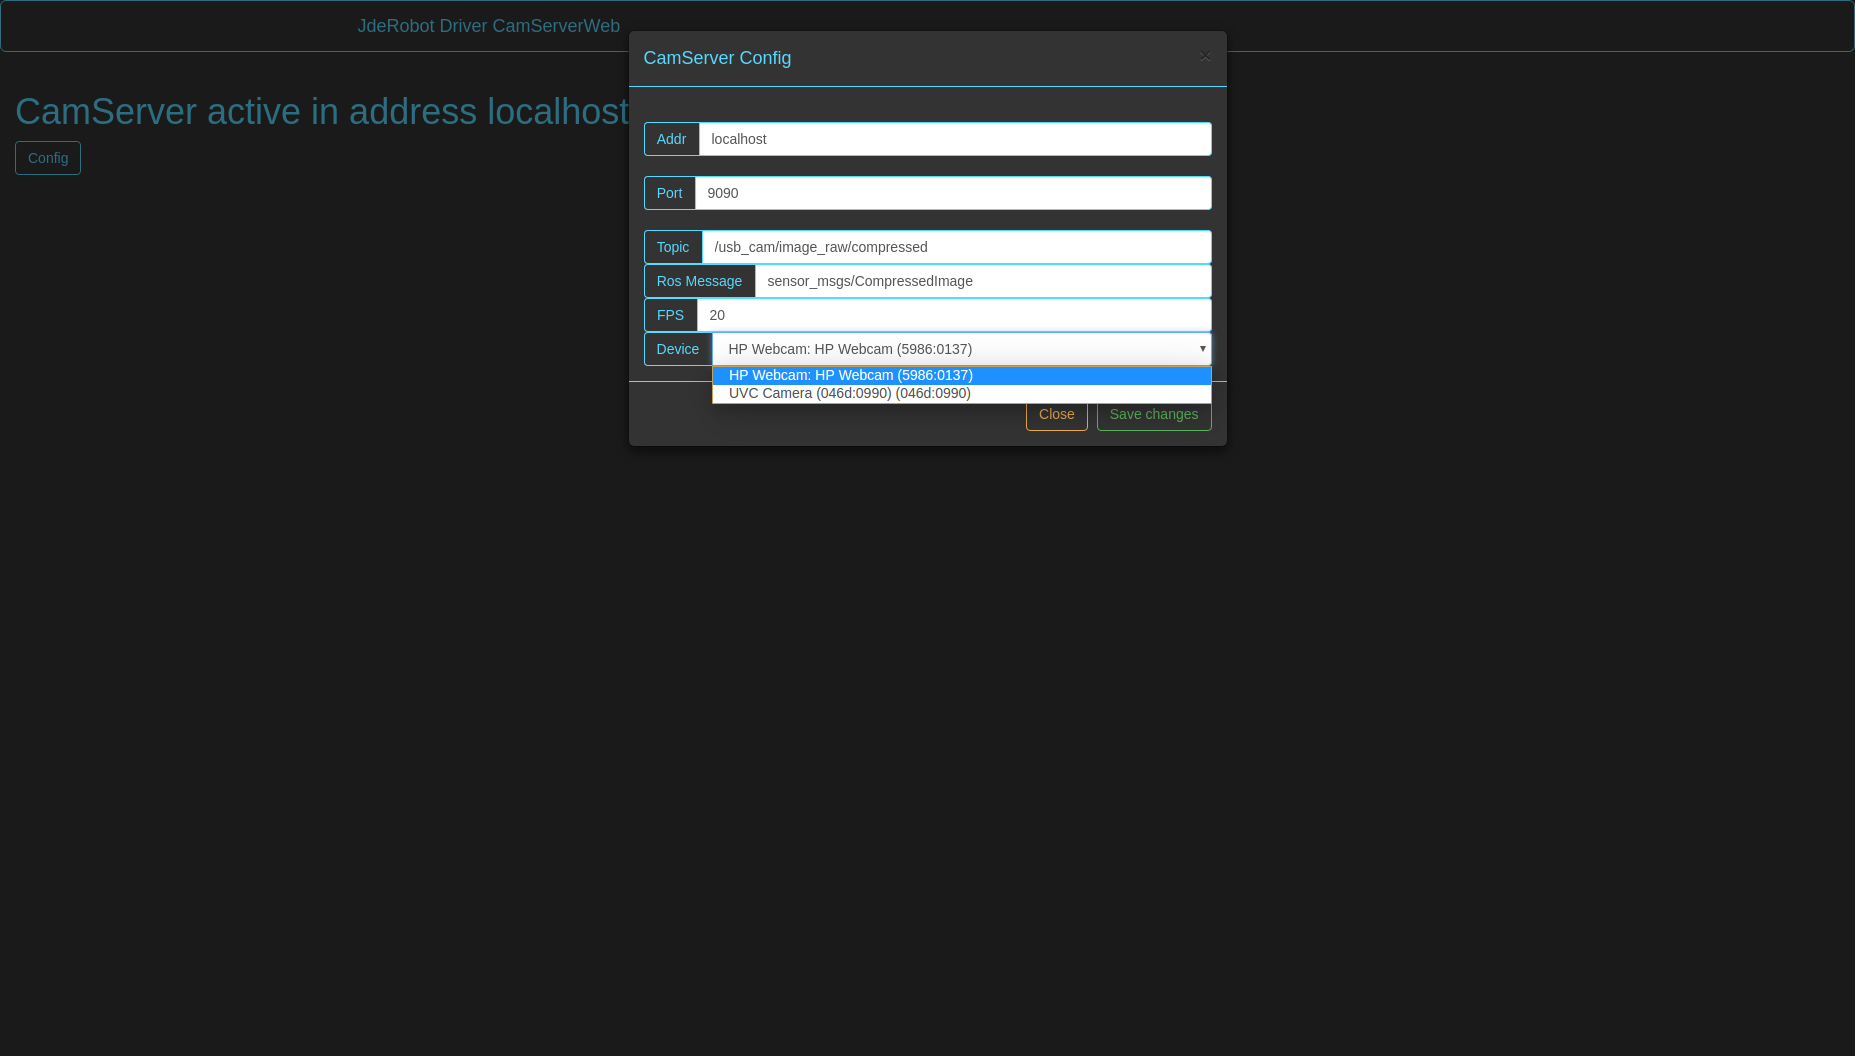
\includegraphics[width=0.8\textwidth]{figures/devicecamserver.png}
		\caption{Selector del dispositivo de entrada de video}
		\label{fig.devicecamserver}
		\end{center}
\end{figure}
Una vez que se selecciona el dispositivo que vamos a utilizar para adquirir las imágenes, hay que conectarse a él. Para esta conexión, se vuelve a utilizar la API de WebRTC, \texttt{Navigator} y el objeto \texttt{Navigator.mediaDevices}, sin embargo en esta ocasión utilizamos el método \texttt{navigator.mediaDevices.getUserMedia(constraints).then(function(stream) \{\})}, donde \texttt{constraints} define los dispositivos multimedia (en este caso el dispositivo de entrada de video escogido) y \texttt{stream} es el flujo de datos obtenido de ellos.

Este flujo de datos está en el formato \texttt{MediaStream}, el cual no es apto para ser enviado o visualizado, por tanto es necesario realizar una conversión. Para realizar la conversión, se va a utilizar el elemento de HTML \texttt{Canvas} y el método JavaScript asociado a este elemento \texttt{toDataURL()}. Este método devuelve un \texttt{data URI} (URLs prefijados que permiten a los creadores de contenido incorporar pequeños archivos en línea en los documentos) que contiene una representación de la imagen en el formato especificado por el parámetro \texttt{type}, tomando en nuestro caso el valor \texttt{image/jpeg}, para obtener las imágenes en el formato comprimido jpeg. Todo está contenido en un canvas virtual, ya que no se mostrará en ningún lugar y únicamente se utiliza como pasarela entre el API de WebRTC y el envío de las imágenes.

\section{Conexiones}
En esta sección se explica cómo se realiza la conexión tipo ROS con la aplicación de visión artificial y el posterior envío de imágenes mediante un \textit{Publisher} de ROS. 

\subsection{Establecimiento de la conexión}
Para realizar la conexión es necesario el uso de la biblioteca roslibjs y que se ha explicado en capítulos anteriores. Esta biblioteca proporciona todo el código necesario para realizar la conexión, indicando si se ha realizado correctamente o a si ha ocurrido algún error. Para realizar la conexión, la biblioteca roslibjs proporciona el objeto \texttt{ROSLIB.Ros}, y el método proporcionado por este objeto, \texttt{ros.on}. El código para establecer la conexión se muestra en el cuadro 6.1.
\begin{lstlisting}[caption= Establecer conexión con ROS, label=cod.conexionRosCamserver]
ros = new ROSLIB.Ros();
ros = new ROSLIB.Ros({
            url : "ws://IP:Puerto"
 });
\end{lstlisting}
En este código, indicaremos que la conexión se hará utilizando un canal de comunicación WebSocket, y la IP y puerto por la que se transmitirá. De esta forma ya se habrá establecido la conexión ROS, pero aún hay que definir el tipo de mensaje a enviar y a través de qué etiqueta de ROS (\textit{topic} de ROS) pueden conectarse las diferentes aplicaciones de visión artificial que deseen obtener las imágenes que se transmiten.

\subsection{Estructura de los mensajes}
El tipo de mensaje que vamos a utilizar para el envío será el tipo predefinido en el API de ROS, \texttt{sensor\_msgs/CompressedImage}. El motivo de la elección de este tipo es debido a que las imágenes se obtienen en formato comprimido jpeg, tal y como se ha explicado en la sección anterior. Sin embargo, este tipo de mensaje no envía información acerca del tamaño de la imagen (altura y anchura), por lo que es necesario enviar otro mensaje adicional para completar esta información. Este mensaje de apoyo es de tipo \texttt{sensor\_msgs/CameraInfo} y transmitirá toda la información sobre la cámara (fotogramas por segundo, altura, anchura, etc). 

Para definir estos dos mensajes, se utiliza el objeto proporcionado por la biblioteca roslibjs, \texttt{ROSLIB.Topic}. A este objeto se le deben introducir como parámetros el objetos \texttt{ROSLIB.Ros} generado para realizar la conexión, el nombre del \textit{topic} y el tipo de mensaje, por lo que generaremos nuestro \textit{Publisher} para servir las imágenes y la información de la cámara mediante el código del cuadro 6.2.
\begin{lstlisting}[caption= Estructura de los mensajes, label=cod.estrucuturamensajes]
var imagenTopic = new ROSLIB.Topic({
	ros:ros, 
	name: config.Topic, 
	messageType : "sensor_msgs/CompressedImage Message"})
	
var cameraInfo = new ROSLIB.Topic({
         ros: self.ros,
         name : "/usb_cam/camera_info",
         messageType: "sensor_msgs/CameraInfo"
       })

\end{lstlisting}

\subsection{Creación de los mensajes y publicación}
Definidos los mensajes y establecida la conexión, el siguiente paso es transmitir los mensajes. Para ello se deben crear los mensajes con la información que se desea transmitir con el \textit{Publisher}, utilizando de nuevo un objeto definido en la biblioteca roslibjs, \texttt{new ROSLIB.Message}. Para crear este objeto, se debe pasar por parámetros el contenido que se quiere que tenga el mensaje, siempre cumpliendo las especificaciones definidas para cada tipo de mensaje escogido anteriormente y que están definidas en la documentación de ROS\footnote{\url{http://wiki.ros.org/common_msgs}}. En este caso, para definir los dos mensajes que transmitiremos lo haremos mediante el código del cuadro 6.3.
\begin{lstlisting}[caption= Definición del mensaje para las imágenes, label=cod.definicionmensajeimg]
 var videomensaje = new ROSLIB.Message({
 	format : "jpeg", 
	data : data.replace("data:image/jpeg;base64,", "")
	})

\end{lstlisting}
Del anterior código cabe destacar que \texttt{data} corresponde a los datos obtenidos mediante el método \texttt{toDataURL} indicado en la sección 6.2, remplazando la cabecera donde se indica el formato, ya que se indica en el propio mensaje mediante \texttt{format}. 

Para el mensaje donde se transmite la información de la cámara usaremos el código del cuadro 6.4.

\begin{lstlisting}[caption= Definición del mensaje para la información de la cámara, label=cod.definicionmensajeinfo]
var camarainfo = new ROSLIB.Message({
	height: imagen.height,
	width: imagen.width})

\end{lstlisting}
Creados los mensajes, solo falta publicarlos, lo que se consigue de una manera sencilla mediante el código que se muestra en el cuadro 6.5.
\begin{lstlisting}[frame=single]
imageTopic.publish(imageMessage);
cameraInfo.publish(infoMessage);
\end{lstlisting}

Se puede apreciar fácilmente que lo que se está realizando es publicar los dos mensajes creados mediante la estructura definida anteriormente. 
Finalmente, es necesario enviar de una manera periódica estos mensajes, ya que con lo indicado anteriormente, únicamente se está enviando un mensaje de cada categoría. 
Para crear un envío periódico, se hace uso del método de JavaScript \texttt{SetInterval()}. Este método llama a una función o evalúa una expresión cuando pase un intervalo de tiempo (en milisegundos), que se indica en la llamada al método junto a la función que se quiere ejecutar cuando se cumpla el citado intervalo.

\section{Configuración}
Para configurar el driver, se ofrecen dos posibilidades:
\begin{itemize}
\item Mediante el uso de un fichero con formato``YAML'' al igual que en resto de herramientas de este trabajo. 
\item Mediante el menú de configuración incorporado en la interfaz gráfica.
\end{itemize}
El primer método realiza la configuración inicial del driver, ya que se configura al arrancar el driver. El segundo método permite realizar la configuración del driver durante la ejecución del mismo, ofreciendo la posibilidad de reconfigurar en tiempo de ejecución sin que sea necesario cerrar y volver a lanzar el driver.

Los parámetros configurables son los siguientes:
\begin{itemize}
\item Dirección IP. Por defecto será localhost.
\item Puerto. Por defecto será 9090.
\item \textit{Topic} al que se deberán registrar los clientes. Por defecto será \texttt{/usb\_cam/image\_raw/compressed}
\item Formato del mensaje. Por defecto será \texttt{sensor\_msgs/CompressedImage}
\item \textit{Framerate}. Por defecto serán 20 fotogramas por segundo.
\item Fuente de video. Por defecto será la primera fuente detectada por WebRTC. Este parámetro únicamente puede ser configurado mediante la configuración en tiempo de ejecución.
\end{itemize}

\subsection{Interfaz gráfica}
La interfaz está realizada mediante HTML y Bootstrap, siguiendo el modelo del resto de aplicaciones web de la plataforma JdeRobot.
\begin{figure}[H]
  \begin{center}
    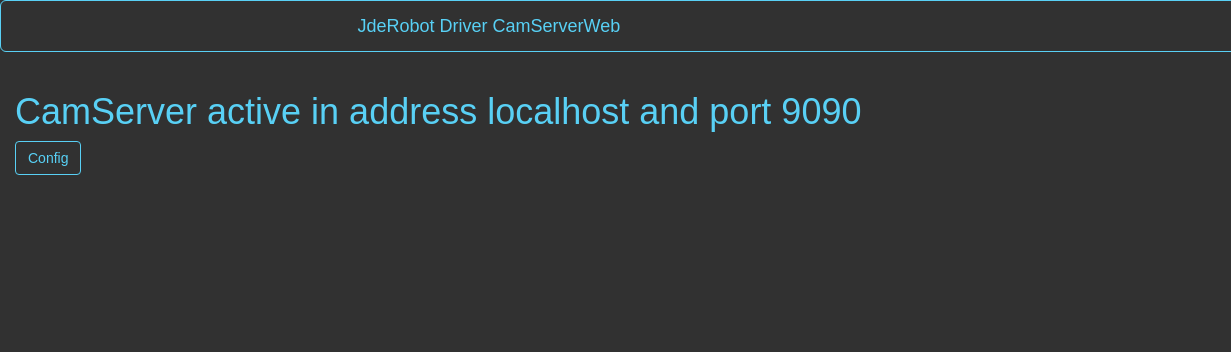
\includegraphics[width=0.8\textwidth]{figures/Interfazcamserver.png}
		\caption{Interfaz gráfica del driver}
		\label{fig.interfazcamserver}
		\end{center}
\end{figure}
La configuración se realiza gracias a un menú desplegable mediante la pulsación de un botón y una vez que se pulse el botón guardar, se almacena la nueva configuración para realizar las conexiones. Este menu se puede apreciar en la figura 6.5.
 \begin{figure}[H]
  \begin{center}
    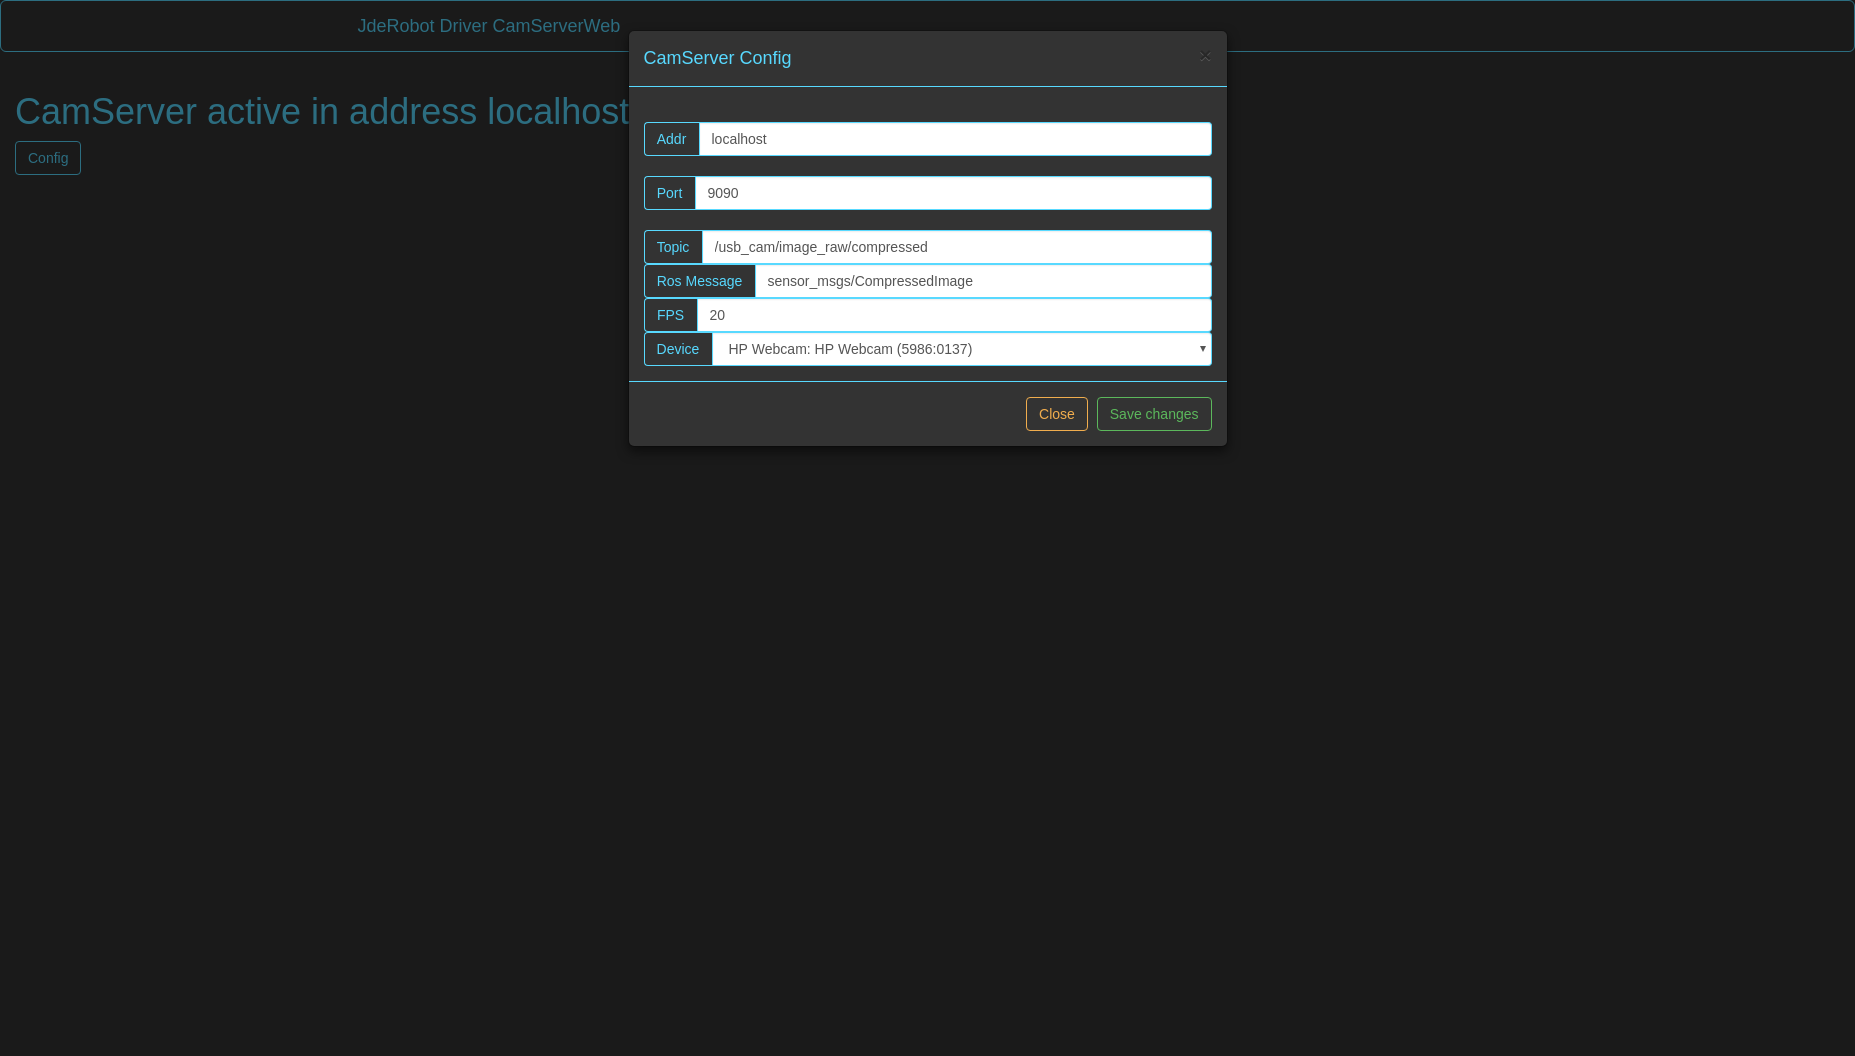
\includegraphics[width=0.8\textwidth]{figures/configcamserver.png}
		\caption{Menú de configuración del servidor de imágenes}
		\label{fig.configcamserver}
		\end{center}
\end{figure}

\section{Experimentos}
Como se ha visto anteriormente, el driver puede ejecutarse a través de dos vías: Electron y Node.js. Sin embargo, la preparación para que funcione correctamente es la misma para ambas vías, siendo la única diferencia la forma de ejecutar el driver.

En un primer terminal o consola se debe ejecutar el servidor intermedio de ROS que se puede ver en el esquema.
\begin{lstlisting}[caption= Ejecución del servidor intermedio, label=cod.servidorintermedio]
roslaunch rosbridge_server rosbridge_websocket.launch
\end{lstlisting}
En un segundo terminal se ejecutará el driver.
\begin{itemize}
\item 
Como aplicación web utilizando Node.js
\end{itemize}
\begin{lstlisting}[caption= Ejecución con Node.js, label=cod.nodejs]
node run.js
Se arranca el navegador y se introduce la URL http://localhost:7777/
\end{lstlisting}
\begin{itemize}
\item 
Como aplicación de escritorio con Electron
\end{itemize}
\begin{lstlisting}[caption= Ejecución con Electron, label=cod.electron]
npm install
npm start
\end{lstlisting}
En ambos casos debemos configurar el driver para que se conecte con el servidor intermedio, en la imagen 4.5 muestra una posible configuración del driver.
\begin{figure}[H]
  \begin{center}
    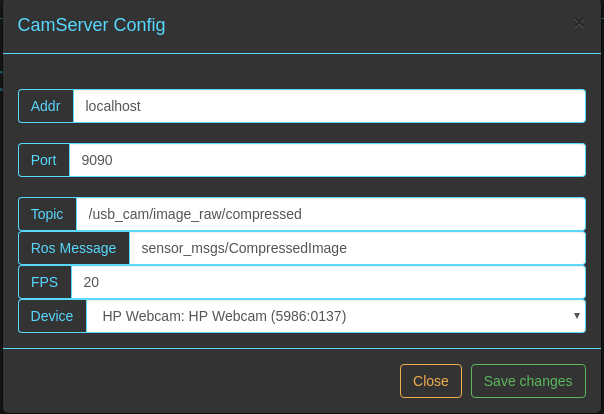
\includegraphics[width=0.8\textwidth]{figures/configcamservertest.png}
		\caption{Ejemplo de configuración del driver}
		\label{fig.esquemacamserver}
		\end{center}
\end{figure}
Finalmente, para verificar que está funcionando correctamente, en un tercer terminal lanzaremos la herramienta rqt\_image\_view, facilitada por ROS para visualizar imágenes enviadas a través de un mensaje de ROS, que hará la función de cliente.

\begin{figure}[H]
  \begin{center}
    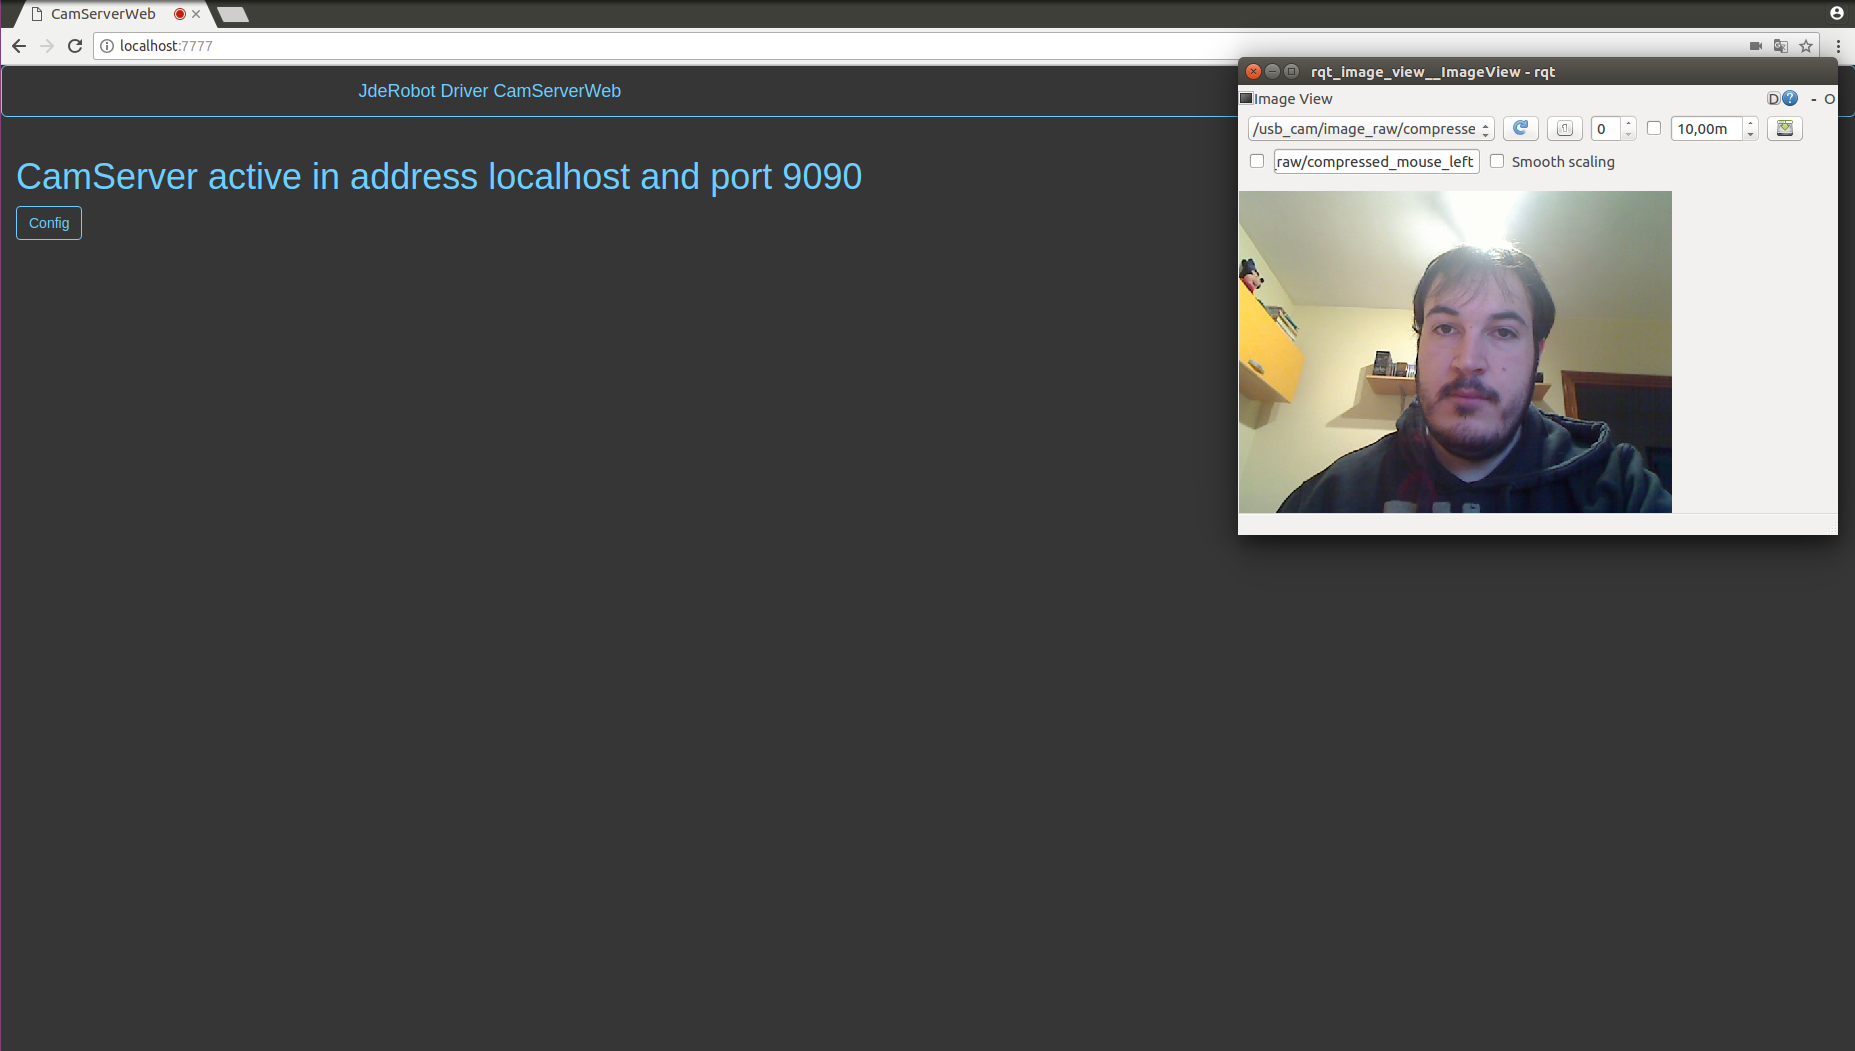
\includegraphics[width=0.8\textwidth]{figures/camservernodejs.png}
    		\caption{CamServerWeb ejecutado en un navegador web}
		\label{fig.testcamserver1}
		\end{center}
\end{figure}
\begin{figure}[H]
  \begin{center}
    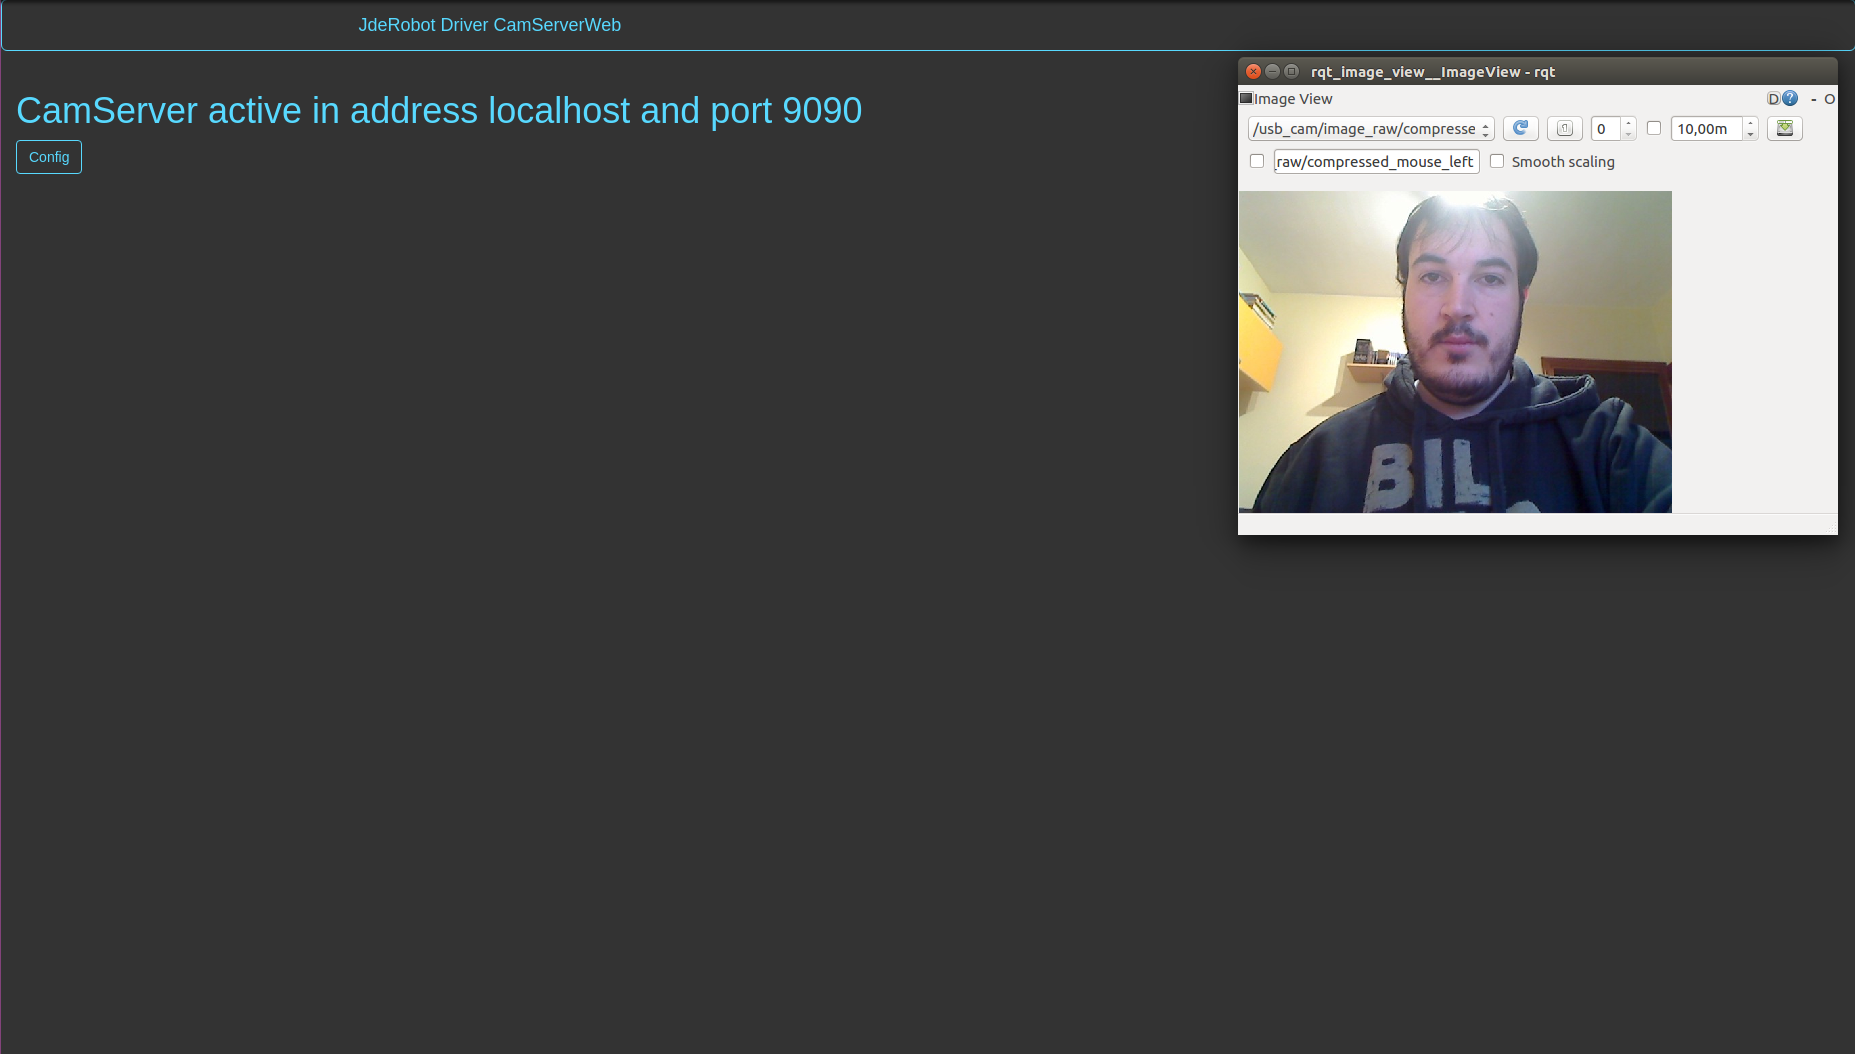
\includegraphics[width=0.8\textwidth]{figures/camserverelectron.png}
    		\caption{CamServerWeb ejecutado en Electron}
		\label{fig.testcamserver2}
		\end{center}
\end{figure}

\lhead[]{CAP\'ITULO \thechapter. CONCLUSIONES}
\chapter{Conclusiones}\label{cap.conclusiones}

Una vez se ha detallado en los últimos capítulos todo el software desarrollado, ha llegado el momento de analizar las contribuciones realizadas y verificar si se han cumplido los objetivos marcados.

\section{Contribuciones}
El principal objetivo marcado en este trabajo era enriquecer las herramientas existentes en la plataforma JdeRobot con nuevas herramientas con tecnologías web. Se puede concluir que se ha alcanzado el objetivo satisfactoriamente realizando la conversión de los visores para su utilización con Electron y ROS, se ha aportado un nuevo visor de elementos 3D y se ha elaborado un nuevo driver para complementar los drivers para fuentes de video ya existentes en la plataforma JdeRobot.

El primer subobjetivo era modificar los tres visores web existentes previamente en la plataforma JdeRobot para que pudieran ser usados tanto en el navegador como con Electron y, a su vez, que pudieran conectarse mediante los middleware ICE y ROS. Como se ha explicado en el capitulo 4 de este trabajo, esta meta se ha alcanzado de manera satisfactoria, teniendo ahora nuevas versiones de los visores llamadas \texttt{CamVizWeb}, \texttt{TurtlebotVizWeb} y \texttt{DroneVizWeb}. Estos tres visores son capaces de comunicarse mediante los middleware de comunicación ICE y ROS, dotándoles de una gran versatilidad al poder conectar un amplio abanico de drivers robóticos.

La segunda meta era crear un nuevo visor 3D con WebGL que sustituyera al visor existente desarrollado en C++, utilizado en la práctica de Robotics Academy de reconstrucción 3D. Este subobjetivo se ha alcanzado con la herramienta web \texttt{3DVizWeb} y, como se ha visto en el capitulo 5, no solo hasta el punto que se había marcado inicialmente (visualización de puntos), sino que se decidió ampliar el visor para que pudiera mostrar también segmentos y objetos 3D. No ha sido posible imitar completamente el funcionamiento del visor anterior, en el nuevo cambia la manera de comunicarse con las aplicaciones. El visor 3D es el encargado de llevar la iniciativa y debe ser él que solicite los elementos al servidor, y no que los reciba sin más como funcionaba anteriormente. Esta herramienta es muy útil para que otros desarrolladores e investigadores puedan representar escenas adquiridas mediante sensores en un mundo tridimensional.

La tercera meta fijada era crear un componente que pudiera obtener y enviar las imágenes obtenidas de una fuente de video WebRTC, complementando a los componentes \texttt{cameraserve}r y \texttt{cameraserver\_py} de JdeRobot que realizan la misma función pero desarrollados con C++ y Python respectivamente. Este subobjetivo se ha alcanzado con el componente \texttt{CamServerWeb} que, como se ha mostrado en el capitulo 6, obtiene imágenes mediante WebRTC de los dispositivos de video conectados y los transmite mediante el middleware de comunicación ROS. Con este componente se da la posibilidad de que cualquier aplicación de visión artificial pueda recibir las imágenes grabadas por las cámaras conectadas a un robot.

Además se ha conseguido que todas las herramientas puedan ser ejecutadas con Electron, lo que permite utilizarlas como una aplicación de escritorio, facilitando su uso por otros usuarios. Gracias a ello, todas las herramientas pueden ejecutarse a través de dos vías (Electron y navegador web) y son multiplataforma.

Analizando todo lo realizado y tras probar su eficiencia mediante las experimentaciones que han resultado exitosas en todos los casos, se puede concluir que se ha enriquecido con tecnologías web la plataforma JdeRobot, que hasta ahora su desarrollo principal era con C++ y Python.

Finalmente, a título personal, he ampliado mis capacidades con tecnologías web y aprendido el uso del entorno Electron que es muy útil para elaborar aplicaciones de escritorio pero programadas como si fueran web. He conocido el mundo de la robótica y como mediante middlewares como ICE o ROS es posible conectar sensores o actuadores a una aplicación para compartir información entre ambos.

\section{Trabajos Futuros}
Todas las herramientas creadas son completamente funcionales y cualquier usuario puede utilizarlas sin problemas, sin embargo existen varios aspectos donde se pueden extender para hacerlas aún más útiles.

\begin{itemize}
\item La primera posibilidad es permitir que tanto la herramienta \texttt{CamVizWeb} como el componente \texttt{CamServerWeb} sean compatibles con las imágenes en crudo de ROS y no solo imágenes comprimidas como ahora. Esta mejora permitiría conectar este visor al resto de drivers de fuentes de video.
\item Otra posibilidad a modificar es conseguir que \texttt{3DVizWeb} reciba los elementos sin que haya realizado la petición previamente, de modo que la iniciativa la lleve enteramente la aplicación y no el visor. Este hecho permitirá que pueda conectarse al visor más de una aplicación simultáneamente, además reducirá el retardo del visor al reducir a la mitad el intercambio de mensajes.
\item Empaquetar las herramientas web mediante paquetes npm, de modo que permita a otros usuarios descargar e instalar fácil y rápidamente las herramientas para ser usadas.
\end{itemize}




%%%%%%%%%%%%%%% Bibliograí­a %%%%%%%%%%%%%%%

\nocite{*}
\lhead[]{BIBLIOGRAF\'IA}
\bibliographystyle{unsrt}
\bibliography{bibliografia}
\addcontentsline{toc}{chapter}{Bibliografía}

\end{document}